%%
%% This is file `sample-acmsmall.tex',
%% generated with the docstrip utility.
%%
%% The original source files were:
%%
%% samples.dtx  (with options: `all,journal,bibtex,acmsmall')
%% 
%% IMPORTANT NOTICE:
%% 
%% For the copyright see the source file.
%% 
%% Any modified versions of this file must be renamed
%% with new filenames distinct from sample-acmsmall.tex.
%% 
%% For distribution of the original source see the terms
%% for copying and modification in the file samples.dtx.
%% 
%% This generated file may be distributed as long as the
%% original source files, as listed above, are part of the
%% same distribution. (The sources need not necessarily be
%% in the same archive or directory.)
%%
%%
%% Commands for TeXCount
%TC:macro \cite [option:text,text]
%TC:macro \citep [option:text,text]
%TC:macro \citet [option:text,text]
%TC:envir table 0 1
%TC:envir table* 0 1
%TC:envir tabular [ignore] word
%TC:envir displaymath 0 word
%TC:envir math 0 word
%TC:envir comment 0 0
%%
%%
%% The first command in your LaTeX source must be the \documentclass
%% command.
%%
%% For submission and review of your manuscript please change the
%% command to \documentclass[manuscript, screen, review]{acmart}.
%%
%% When submitting camera ready or to TAPS, please change the command
%% to \documentclass[sigconf]{acmart} or whichever template is required
%% for your publication.
%%
%%
\documentclass[acmsmall,screen,review,anonymous]{acmart}

%%
%% \BibTeX command to typeset BibTeX logo in the docs
\AtBeginDocument{%
  \providecommand\BibTeX{{%
    Bib\TeX}}}

%% Rights management information.  This information is sent to you
%% when you complete the rights form.  These commands have SAMPLE
%% values in them; it is your responsibility as an author to replace
%% the commands and values with those provided to you when you
%% complete the rights form.
\setcopyright{acmlicensed}
\copyrightyear{2024}
\acmYear{2024}
\acmDOI{XXXXXXX.XXXXXXX}


%%
%% These commands are for a JOURNAL article.
\acmJournal{JACM}
\acmVolume{37}
\acmNumber{4}
\acmArticle{111}
\acmMonth{8}

%%
%% Submission ID.
%% Use this when submitting an article to a sponsored event. You'll
%% receive a unique submission ID from the organizers
%% of the event, and this ID should be used as the parameter to this command.
%%\acmSubmissionID{123-A56-BU3}

%%
%% For managing citations, it is recommended to use bibliography
%% files in BibTeX format.
%%
%% You can then either use BibTeX with the ACM-Reference-Format style,
%% or BibLaTeX with the acmnumeric or acmauthoryear sytles, that include
%% support for advanced citation of software artefact from the
%% biblatex-software package, also separately available on CTAN.
%%
%% Look at the sample-*-biblatex.tex files for templates showcasing
%% the biblatex styles.
%%

%%
%% The majority of ACM publications use numbered citations and
%% references.  The command \citestyle{authoryear} switches to the
%% "author year" style.
%%
%% If you are preparing content for an event
%% sponsored by ACM SIGGRAPH, you must use the "author year" style of
%% citations and references.
%% Uncommenting
%% the next command will enable that style.
%%\citestyle{acmauthoryear}

% Language setting
% Replace `english' with e.g. `spanish' to change the document language
\usepackage[english]{babel}
\usepackage{subcaption}
% Useful packages
\usepackage{amsmath}
\usepackage{graphicx}
\graphicspath{{figures/}}
%\usepackage{amssymb}
\usepackage{mathtools}
\usepackage{array}
\usepackage{minted}
\usepackage{ifthen}
\usepackage{ebproof}
\ebproofset{label separation=0pt}
\usepackage{multirow}
\usepackage{wrapfig}


\makeatletter
\DeclareFontFamily{OMX}{MnSymbolE}{}
\DeclareSymbolFont{MnLargeSymbols}{OMX}{MnSymbolE}{m}{n}
\SetSymbolFont{MnLargeSymbols}{bold}{OMX}{MnSymbolE}{b}{n}
\DeclareFontShape{OMX}{MnSymbolE}{m}{n}{
    <-6>  MnSymbolE5
   <6-7>  MnSymbolE6
   <7-8>  MnSymbolE7
   <8-9>  MnSymbolE8
   <9-10> MnSymbolE9
  <10-12> MnSymbolE10
  <12->   MnSymbolE12
}{}
\DeclareFontShape{OMX}{MnSymbolE}{b}{n}{
    <-6>  MnSymbolE-Bold5
   <6-7>  MnSymbolE-Bold6
   <7-8>  MnSymbolE-Bold7
   <8-9>  MnSymbolE-Bold8
   <9-10> MnSymbolE-Bold9
  <10-12> MnSymbolE-Bold10
  <12->   MnSymbolE-Bold12
}{}

\let\llangle\@undefined
\let\rrangle\@undefined
\DeclareMathDelimiter{\llangle}{\mathopen}%
                     {MnLargeSymbols}{'164}{MnLargeSymbols}{'164}
\DeclareMathDelimiter{\rrangle}{\mathclose}%
                     {MnLargeSymbols}{'171}{MnLargeSymbols}{'171}
\makeatother

% Configuration for minted package
\setminted{
    style=colorful, % Set code style to colorful
    fontsize=\tiny,
    linenos=false, % Enable line numbers
    breaklines, % Enable line breaks
    breakanywhere, % Allow line breaks anywhere
    autogobble,
}
\setmintedinline{fontsize=\small}
%\usepackage[colorlinks=true, allcolors=blue]{hyperref}


\ifthenelse{1=0}{
\newcommand{\TODO}[1]{\textcolor{red}{TODO: #1}}
\newcommand\help[1]{\textcolor{green}{Help Needed: #1}}
\newcommand\kyle[1]{\textcolor{olive}{Kyle: #1}}
\newcommand\teo[1]{\textcolor{red}{teo: #1}}
\newcommand\willow[1]{\textcolor{purple}{Willow: #1}}
\newcommand{\saman}[1]{\textcolor{orange}{Saman: #1}}
\newcommand{\leftoff}{\textcolor{red}{\textbf{LEFT OFF}}}
\newcommand\changwan[1]{\textcolor{blue}{CW: #1}}
}{
\newcommand{\TODO}[1]{}
\newcommand{\help}[1]{}
\newcommand{\saman}[1]{}
\newcommand{\kyle}[1]{}
\newcommand{\teo}[1]{}
\newcommand{\willow}[1]{}
\newcommand{\leftoff}{}
}

\newcommand{\finchextent}{\ensuremath{\text{\textbf{extent}}}}
\newcommand{\finchliteral}{\ensuremath{\text{\textbf{literal}}}}
\newcommand{\finchvalue}{\ensuremath{\text{\textbf{value}}}}
\newcommand{\finchtensor}{\ensuremath{\text{\textbf{tensor}}}}
\newcommand{\finchmode}{\ensuremath{\text{\textbf{mode}}}}
\newcommand{\finchindex}{\ensuremath{\text{\textbf{index}}}}
\newcommand{\finchvar}{\ensuremath{\text{\textbf{variable}}}}
\newcommand{\finchcall}{\ensuremath{\text{\textbf{call}}}}
\newcommand{\finchaccess}{\ensuremath{\text{\textbf{access}}}}
\newcommand{\finchread}{\ensuremath{\text{\textbf{read}}}}
\newcommand{\finchassign}{\ensuremath{\text{\textbf{assign}}}}
\newcommand{\finchupdate}{\ensuremath{\text{\textbf{update}}}}
\newcommand{\finchloop}{\ensuremath{\text{\textbf{loop}}}}
\newcommand{\finchdefine}{\ensuremath{\text{\textbf{define}}}}
\newcommand{\finchsieve}{\ensuremath{\text{\textbf{sieve}}}}
\newcommand{\finchblock}{\ensuremath{\text{\textbf{block}}}}
\newcommand{\finchdeclare}{\ensuremath{\text{\textbf{declare}}}}
\newcommand{\finchfreeze}{\ensuremath{\text{\textbf{freeze}}}}
\newcommand{\finchthaw}{\ensuremath{\text{\textbf{thaw}}}}

\newcommand{\finchthunk}{\ensuremath{\text{\textbf{thunk}}}}
\newcommand{\finchphase}{\ensuremath{\text{\textbf{phase}}}}
\newcommand{\finchswitch}{\ensuremath{\text{\textbf{switch}}}}
\newcommand{\finchlookup}{\ensuremath{\text{\textbf{lookup}}}}
\newcommand{\finchrun}{\ensuremath{\text{\textbf{run}}}}
\newcommand{\finchspike}{\ensuremath{\text{\textbf{spike}}}}
\newcommand{\finchsequence}{\ensuremath{\text{\textbf{sequence}}}}
\newcommand{\finchstepper}{\ensuremath{\text{\textbf{stepper}}}}


\newcommand{\finchplan}{\ensuremath{\text{\textbf{plan}}}}
\newcommand{\finchquery}{\ensuremath{\text{\textbf{query}}}}
\newcommand{\finchtable}{\ensuremath{\text{\textbf{table}}}}
\newcommand{\finchalias}{\ensuremath{\text{\textbf{alias}}}}
\newcommand{\finchmapjoin}{\ensuremath{\text{\textbf{mapjoin}}}}
\newcommand{\finchaggregate}{\ensuremath{\text{\textbf{aggregate}}}}
\newcommand{\finchrelabel}{\ensuremath{\text{\textbf{relabel}}}}
\newcommand{\finchreorder}{\ensuremath{\text{\textbf{reorder}}}}
\newcommand{\finchreformat}{\ensuremath{\text{\textbf{reformat}}}}


\newcommand{\HIDE}[1]{}

\newcommand{\rothead}[1]{\rotatebox{90}{\textbf{#1}}}



%%
%% end of the preamble, start of the body of the document source.
\begin{document}


%%
%% The "title" command has an optional parameter,
%% allowing the author to define a "short title" to be used in page headers.
\title{Finch: Sparse and Structured Array Programming with Control Flow}

%%
%% The "author" command and its associated commands are used to define
%% the authors and their affiliations.
%% Of note is the shared affiliation of the first two authors, and the
%% "authornote" and "authornotemark" commands
%% used to denote shared contribution to the research.
\author{Willow Ahrens}
\affiliation{%
  \institution{MIT CSAIL}
  \city{Cambridge}
  \state{Massachusetts}
  \country{USA}}
\email{willow@csail.mit.edu}

\author{Teodoro Fields Collin}
\affiliation{%
  \institution{MIT CSAIL}
  \city{Cambridge}
  \state{Massachusetts}
  \country{USA}}
\email{teoc@mit.edu}

\author{Radha Patel}
\affiliation{%
  \institution{MIT CSAIL}
  \city{Cambridge}
  \state{Massachusetts}
  \country{USA}}
\email{rrpatel@mit.edu}

\author{Kyle Deeds}
\affiliation{%
  \institution{University of Washington}
  \city{Seattle}
  \state{Washington}
  \country{USA}}
\email{kdeeds@cs.washington.edu}

\author{Changwan Hong}
\affiliation{%
  \institution{MIT CSAIL}
  \city{Cambridge}
  \state{Massachusetts}
  \country{USA}}
\email{changwan@mit.edu}

\author{Saman Amarasinghe}
\affiliation{%
  \institution{MIT CSAIL}
  \city{Cambridge}
  \state{Massachusetts}
  \country{USA}}
\email{saman@csail.mit.edu}

%%
%% By default, the full list of authors will be used in the page
%% headers. Often, this list is too long, and will overlap
%% other information printed in the page headers. This command allows
%% the author to define a more concise list
%% of authors' names for this purpose.
\renewcommand{\shortauthors}{Ahrens et al.}

%%
%% The abstract is a short summary of the work to be presented in the
%% article.
\begin{abstract}
From FORTRAN to Numpy, arrays have revolutionized how we express computation. However, arrays in these, and almost all prominent systems, can only handle dense rectilinear integer grids.  Real world arrays often contain underlying structure, such as sparsity, runs of repeated values, or symmetry.  Support for structured data is fragmented and incomplete.  Existing frameworks limit the array structures and program control flow they support to better simplify the problem.

In this work, we propose a new programming language, Finch, which supports \textit{both} flexible control flow and diverse data structures. Finch facilitates a programming model which resolves the challenges of computing over structured arrays by combining control flow and data structures into a common representation where they can be co-optimized. In particular, Finch automatically specializes the control flow to the data so that performance engineers can focus on experimenting with many algorithms. Finch supports a familiar programming language of loops, statements, if conditions, breaks, etc., over a wide variety of array structures, such as sparsity, run-length-encoding, symmetry, triangles, padding, or blocks. Finch reliably utilizes the key properties of structure, such as structural zeros, repeated values, or clustered non-zeros. We show that this leads to dramatic speedups in operations such as spmv and spgemm, image processing, graph analytics, and a high-level tensor operator fusion interface.
\end{abstract}

%%
%% The code below is generated by the tool at http://dl.acm.org/ccs.cfm.
%% Please copy and paste the code instead of the example below.
%%
\begin{CCSXML}
  <ccs2012>
  <concept>
  <concept_id>10011007.10011006.10011008.10011024.10011027</concept_id>
  <concept_desc>Software and its engineering~Control structures</concept_desc>
  <concept_significance>500</concept_significance>
  </concept>
  <concept>
  <concept_id>10011007.10011006.10011008.10011024.10011028</concept_id>
  <concept_desc>Software and its engineering~Data types and structures</concept_desc>
  <concept_significance>500</concept_significance>
  </concept>
  <concept>
  <concept_id>10011007.10011006.10011008.10011009.10011010</concept_id>
  <concept_desc>Software and its engineering~Imperative languages</concept_desc>
  <concept_significance>300</concept_significance>
  </concept>
  <concept>
  <concept_id>10002950.10003705</concept_id>
  <concept_desc>Mathematics of computing~Mathematical software</concept_desc>
  <concept_significance>500</concept_significance>
  </concept>
</ccs2012>
\end{CCSXML}
  
\ccsdesc[500]{Software and its engineering~Control structures}
\ccsdesc[500]{Software and its engineering~Data types and structures}
\ccsdesc[300]{Software and its engineering~Imperative languages}
\ccsdesc[500]{Mathematics of computing~Mathematical software}
%%
%% Keywords. The author(s) should pick words that accurately describe
%% the work being presented. Separate the keywords with commas.
\keywords{Sparse Array, Structured Array, Control Flow, Programming Language}

\received{20 February 2007}
\received[revised]{12 March 2009}
\received[accepted]{5 June 2009}

%%
%% This command processes the author and affiliation and title
%% information and builds the first part of the formatted document.
\maketitle

\section{Introduction}

%Array programming is the core abstraction behind many of the modern miracles of computing (e.g. neural networks, scientific simulation, database processing). 
Arrays are the most fundamental abstraction in computer science. Arrays and lists are often the first-taught datastructure
\cite[Chapter 2.2]{abelson_structure_1996}, \cite[Chapter 2.2]{knuth_art_1997}.
%
Arrays are also universal across programming languages, from their introduction
in Fortran in 1957 to present-day languages like Python
\cite{backus_fortran_1957}, keeping more-or-less the same semantics.
%
Modern array programming languages such as NumPy~\cite{harris_array_2020},
SciPy~\cite{virtanen_scipy_2020}, MatLab~\cite{moler_history_2020},
TensorFlow~\cite{abadi_tensorflow_2016}, PyTorch~\cite{paszke_pytorch_2019}, and
Halide~\cite{ragan-kelley_halide_2013} have pushed the limits of productive data
processing with arrays, fueling breakthroughs in machine learning, scientific
computing, image processing, and more.
% EASY CUT
%These frameworks have been the
%subject of extensive industry investment to enable performant implementations,
%and often operate at the peak capacity of the hardware they run on
%\cite{lo_roofline_2015}.

The success and ubiquity of arrays is largely due to their simplicity. 
%
Since their introduction, multidimensional arrays have represented dense, rectilinear,
integer grids of points. 
%
By \textbf{dense}, we mean that indices are mapped to value via a simple formula relating multidimensional space to linear memory.
%
Consequently, dense arrays offer extensive compiler optimizations and many convenient interfaces.
%
%This
%simplicity enables extensive interoperability, convenience layers, and
%optimizations by breaking the abstraction barrier between array representation
%and array storage.  
%
Compilers understand dense array computations across many
programming constructs, such as for and while loops, breaks, parallelism,
caching, prefetching, multiple outputs, scatters, gathers, vectorization,
loop-carry-dependencies, and more. A myriad of optimizations have been developed for
dense arrays, such as loop fusion, loop tiling, loop unrolling, and loop
interchange.
%
However, while dense arrays are the easiest way to program for performance, the world is not all dense.

\begin{figure}
	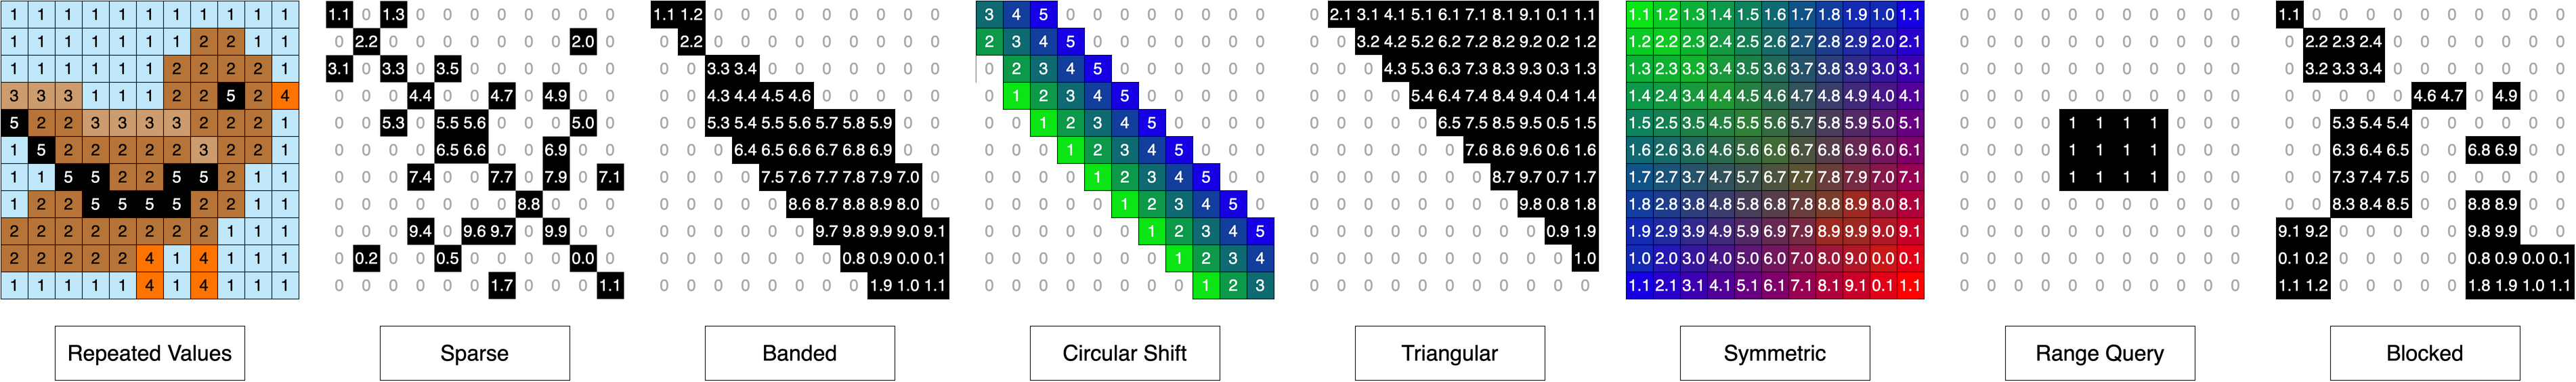
\includegraphics[width=\linewidth]{Structures-examples.png}
    \caption{A few examples of matrix structures arising in practice}
\end{figure}
Our world is full of structured arrays.
%
Sparse arrays (which store only nonzero elements) describe networks, databases, and simulations~\cite{abhyankarpetsc, bell2007lessons, mcauley2013hidden, balay2020petsc}.
%
Run-length encoding describes images and masks, geometry, and
databases (such as a list of transactions with the date field all the same)~\cite{shi2020column,golomb1966run}.
%
Symmetry, bands, padding, and blocks arise due to modeling choices in scientific computing (e.g. higher order FEMs) as well as in intermediate structures in many linear solvers (e.g. GMRES)~\cite{ded, saad2003iterative, o2009scientific}.
%
In the context of machine learning, combinations of sparse and blocked matrices are increasingly under consideration~\cite{dao2022monarch}.
%
Operators, such as convolution, can be expressed as structured arrays.
%
For example, a convolution with a filter can be expressed as a matrix multiplication
with the toeplitz matrix of all the circular shifts of the filter~\cite{sze2017efficient}.

%
\textbf{Currently, support for structured data is fragmented and incomplete}.
%
Experts must hand write variations of even the simplest kernels, like matrix
multiply, for each data structure/data set and architecture to get performance.
%
Implementations must choose a small set of features to support well, resulting
in a compromise between \textbf{program flexibility} and \textbf{data structure
flexibility}.
%
Hand-written solutions are collected in diverse libraries like
MKL, OpenCV, LAPACK or SciPy~\cite{ bradski2000opencv, anderson1999lapack, virtanen2020scipy, psarras2022linear}. 
%
However, libraries will only ever support a subset of
programs on a subset of data structure combinations.
%
Even the most advanced
libraries, such as the GraphBLAS, which support a wide variety of sparse
operations over various semi-rings always lack support for other features, such
as tensors, fused outputs, or runs of repeated values~\cite{bulucc2017design, mattson2019lagraph}.
%
While dense array
compilers support an enormous variety of program constructs like early break and
multiple left hand sides, they only support dense arrays~\cite{ragan-kelley_halide_2013,grosser2012polly}.  
%
Special-purpose
compilers like TACO~\cite{kjolstad_tensor_2019}, Taichi~\cite{hu_taichi_2019}, StructTensor~\cite{ghorbani2023compiling}, or CoRa~\cite{fegade_cora_2022} which support a select subset of structured data
structures (only sparse, or only ragged arrays) must compromise by greatly
constraining the classes of programs which they support, such as tensor
contractions.
%
This trade-off is visualized in Tables \ref{tab:features} and \ref{tab:data_structures}.
%

\newcommand*\rot{\rotatebox{90}}

\begin{table}[h!]
\noindent
\flushleft
\begin{minipage}[t]{.49\textwidth}
  \scriptsize
  \begin{tabular}{l|cccccc}
  \textbf{Feature / Tool} & \rothead{Halide} & \rothead{Taco} & \rothead{Cora} & \rothead{Taichi} & \rothead{Stur} & \rothead{Finch} \\
  \hline
  Einsums/Contractions & \checkmark & \checkmark & \checkmark & \checkmark & \checkmark & \checkmark \\
  % High-Level API           &            & \checkmark &            &            &            & \checkmark \\
  % Automatic API Fusion     &            &            &            &            &            & \checkmark \\
%  Parallelism             & \checkmark & \checkmark & \checkmark & \checkmark&           & \checkmark \\
  Multiple LHS             & \checkmark &            & \checkmark & \checkmark &            & \checkmark \\
  Affine Indices           & \checkmark &            &            & \checkmark & \checkmark & \checkmark \\
  Recurrence               & \checkmark &            &            &            &            &           \\
  If-Conditions and Masks  & \checkmark & \checkmark &            & \checkmark &            & \checkmark \\
  Scatter Gather           & \checkmark &            &            & \checkmark &            &\checkmark \\
  Early Break              &            & \checkmark &            & \checkmark &            &\checkmark \\
  Unrestricted Read/Write              &    \checkmark        &  &            &  &            &  \\
  \end{tabular}
  \caption{Control flow support across various tools.}
  \label{tab:features}
\end{minipage} 
\begin{minipage}[t]{.49\textwidth}
  \flushright
  \scriptsize
  \begin{tabular}{l|cccccc}
  \textbf{Feature / Tool} & \rothead{Halide} & \rothead{Taco} & \rothead{Cora} & \rothead{Taichi} & \rothead{Stur} & \rothead{Finch} \\
  \hline
  Dense                    & \checkmark & \checkmark & \checkmark & \checkmark & \checkmark & \checkmark \\
  Padded                   & \checkmark &            &            &            &            & \checkmark \\
  One Sparse Operand              &            & \checkmark &            & \checkmark &            &\checkmark \\
  Multiple Sparse  Operands                 &            & \checkmark &            &            &            &\checkmark \\
  Run-length               &            &            &            &            &            & \checkmark \\
  Symmetric                &            &            &            &            & \checkmark & \checkmark \\
  Regular Sparse Blocks    &            & \checkmark &            &            &            & \checkmark \\
  Irregular Sparse Blocks  &            &            &            &            &            &\checkmark \\
  Ragged                   &            &            & \checkmark &            &            & \checkmark \\
  \end{tabular}
  \caption{Data structure support across various tools.  Finch supports \textbf{both} complex programs and complex data structures.}
  \label{tab:data_structures}
\end{minipage}
\vspace{-24pt}
\end{table}


%
Prior implementations are incomplete because the abstractions they use are tightly coupled with the specific data structures that they support.
%
For example, TACO merge lattices represent boolean logic over sets of non-zero values on an integer grid~\cite{kjolstad_tensor_2017}.
%
The polyhedral model allows various compilers to represent dense computations on affine regions~\cite{grosser2012polly}.
%
Taichi enriches single static assignment form with a specialized instruction for accessing only a single sparse structure, but it supports more control flow ~\cite{hu_taichi_2019}.
These systems tightly couple their control flow to narrow classes of data structures to avoid the challenges that occur when we intersect complex control flow with structured data. There are two challenges:
%writing efficient code over structured data


\textbf{Optimizations are specific to the indirection and patterns in data structures}: 
%
These structures break the simple mapping between array elements and where they are stored in memory.
%
For example, sparse arrays store lists of which coordinates are nonzero, whereas run-length-encoded arrays map several pixels to the same color value. 
%
These zero regions or repeated regions are optimization opportunities, and we must adapt the program to avoid repetitive work on these regions by referencing the stored structure.

\textbf{Performance on structured data is highly algorithm dependent}: The landscape of implementation decisions is dramatically unpredictable. 
%
For example, the asymptotic performance of sparse matrix multiplication can be impacted by the distribution of nonzeros, the sparse format, and the loop order~\cite{ahrens2022autoscheduling, zhang2021gamma}. 
%For example, sparse kernels don't need to compute on zeros, but this means that the precise input nonzero patterns act as computational filters, affecting the runtime as they interact with each other and the implementation.
This means that performance engineering for such kernels requires the exploration of a large design space, changing the algorithm as well as the data structures.



\textbf{In this work, we propose a new programming language, Finch, which supports \textit{both} flexible control flow and diverse data structures.}
%
Finch facilitates a programming model which resolves the challenges of computing over structured arrays by \textbf{combining control flow and data structures into a common representation where they can be co-optimized}.
%
In particular, Finch automatically specializes the control flow to the data so that performance engineers can focus on experimenting with many algorithms.
%
Finch supports a familiar programming language of loops, statements, if conditions, breaks, etc, over a wide variety of array structures, such as sparsity, run-length-encoding, symmetry, triangles, padding, or blocks. 
%
This support would be useless without the appropriate level of structural specialization; Finch reliably utilizes the key properties of structure, such as structural zeros, repeated values, or clustered non-zeros.
%

As an example, a programmer might explore different ways to intersect only the even integers of two lists (represented as sparse vectors with sorted indices). The control flow here is only useful if the first example differs from the next two in that it actually selects only even indices as the two integer lists are merged and different from the last in that it does not require another tensor:
%The Finch compiler uses the structure of the data to generate efficient implementations of these programs.

%\teo{Proposed new paragraph:}
%\teo{Add: }
%\teo{We don't propose to solve these problems automatically, but we do propose a new programming language where these issues are solvable, by virtue of the precise manner in which we combine structured data and control flow.}
%
%\teo{Our language, Finch, combines structured data and control flow in a predictable manner by lowering both of them into a single abstraction} Looplets~\cite{ahrens_looplets_2023}, which combines structured iterators into a single control flow that only produces the relevant portions of the output.}
%
%\teo{For example, if a programmer wanted to merge the even indices of two sorted arrays, a programmer could represent by point-wise multiplying two sparse vectors to produce another sparse vector and then set the even indices two zero or the programmer could only point-wise multiply the two sparse vectors under an if condition that selects even indices. (This crucial part needs improvement)}
%
%\teo{Via index expressions, multiple levels of loops and tensors, and more complex filtering expressions, we can imagine many variation of this problem with fine grained distinctions about when various operations are performed.}


\begin{minipage}{0.25\linewidth}
\begin{minted}{julia}
     for i = _
         if i % 2 == 0
             c[i]=a[i]*b[i]
         end
     end
\end{minted}
\end{minipage}%
\begin{minipage}{0.25\linewidth}
\begin{minted}{julia}
     for i = _
         if i % 2 == 0
             ap[i] = a[i]
         end
     end
     for i = _
         c[i] = ap[i] * b[i]
     end
\end{minted}
\end{minipage}%
\begin{minipage}{0.25\linewidth}
\begin{minted}{julia}
     for i = _
         cp[i] = a[i] * b[i]
     end
     for i = _
         if i % 2 == 0
             c[i] = cp[i]
         end
     end
\end{minted}
\end{minipage}%
\begin{minipage}{0.25\linewidth}
\begin{minted}{julia}
     for i = _
        if i % 2 == 0
            f[i] = 1
        end
     end
     for i = _
        c[i] = a[i] * b[i] * f[i]
     end
\end{minted}
\end{minipage}%

\subsection{Contributions}


\begin{enumerate}
\item More complex array structures than ever before. We are the first to extend level-by-level hierarchical descriptions to capture banded, triangular, run-length-encoded, or sparse datasets, and any combination thereof.
%
We have chosen a set of level formats that completely captures all combinations of relevant structural properties (zeros, repeated values, and/or blocks).
%
Although many systems (TACO, Taichi, SPF, Ebb)~\cite{chou2018format,  hu_taichi_2019, strout2018sparse, bernstein2016ebb} feature a flexible structure description, our level abstraction is more capable and extensible because it uses Looplets \cite{ahrens_looplets_2023} to express the structure of each level. 
%
\item A rich structured array programming language with for-loops and complex control flow constructs at the same level of productivity of dense arrays. 
%
To our knowledge, the Finch programming language is the first to support if-conditions, early breaks, and multiple left hand sides over structured data, as well as complex accesses such as affine indexing or scatter/gather of sparse or structured operands.
%
\item A compiler that specializes programs to data structures automatically, facilitating an expressive language that makes it easier to search the complex space of algorithms and data structures. Finch reliably utilizes four key properties of structure, such as structural zeros, repeated values, clustered non-zeros, and singletons.
%
\item Our compiler is highly extensible, evidenced by the variety of level formats and control flow constructs we implement in this work.
%
For example, Finch has been extended to support real-valued array indices with continuous arrays \cite{won2024continuous}.
%
\item We evaluate the efficiency, flexibility, and expressability of our language in several case studies, showing that Finch can be used to accelerate a wide range of applications,  from classic operations such as spmv and spgemm, to more complex applications such as image processing, graph analytics, and a high-level tensor operator fusion interface.
%We also demonstrate how Finch can fuse high-level operations to achieve a significant speedup over non-fused kernels. Additionally, as a case study, a high-level array programming language and fusion interface for operations such as map, broadcast, or reduce that can be compiled to efficient code using the previous loop-level abstractions.
%\item A complete set of level formats for expressing data patterns hierarchically in FiberTree-style decompositions. The first such set of formats to efficiently capture banded, triangular, run-length-encoded, or sparse-run-length-encoded datasets. The formats capture many use cases, from random updates to sequential construction.
%\item The Finch array language, mirroring simple for-loops with imperative code blocks and if-conditions. The first array programming language for the above data formats to support multiple outputs, affine indexing, and imperfectly-nested loops.
%\item Tensor lifecycles, a simple constraint on tensor reads and writes that elegantly restricts Finch programs to avoid complex data dependencies, and enables tensor polymorphism by providing implementers with well-defined functions to overload.
%\item Wrapper Tensors which modify existing datastructures and recombine them to support new patterns, such as affine indexing, padding, transposition, and slicing.
%\item Wrapper Levels which modify existing datastructures and enabling complex features such as atomic updates or contiguous versus separate allocation.
%\item We define the first mappings from the existing pydata/sparse array api high-level operations to low level finch notation
%\item <Performance Contributions>

\end{enumerate}

This advances the state of the art over the Looplets work, as the Looplets presented a way to merge iterators over multiple single dimensional structures, whereas we present a way to combine single-dimensional looplet structures into multi-dimensional tensors and operate on them with a programming language with fully-featured control flow.

\section{Background On Looplets}
Finch represents iteration patterns using Looplets, a language that decomposes datastructure iterators hierarchically. 
%
Looplets represent the control-flow structures needed to iterate over any given datastructure, or multiple datastructures simultaneously. 
%
In particular, looplets are good at lifting code to the highest loop level that it's needed and subdividing iteration hierarchically in coordinate space.
%
Because looplets are compiled with progressive lowering, structure-specific mathematical optimizations such as integrals, multiply by zero, etc. can be implemented using simple compiler passes like term rewriting and constant propagation during the intermediate lowering stages \cite{ahrens_looplets_2023}.

The looplets are described in Figure~\ref{fig:looplets}. We simplify the presentation to focus on the semantics, rather than precise implementation.  Several looplets introduce or modify variables in the scope of the target language. It is assumed that if a looplet introduces a variable to be used in a child looplet, the child looplet will not modify that variable.

% \begin{figure}[ht]
%     \footnotesize
%     \begin{minipage}[c]{0.65\linewidth}
%         $\finchlookup(seek, body)$: The Lookup Looplet represents a
%         randomly accessible region of an iterator. The body of the lookup is
%         understood to have one less dimension than the lookup itself, as we have
%         already ``looked up'' that index in the tensor by the time we reach the
%         body. \texttt{seek(i)} is a function that updates state to the given
%         index.
%     \end{minipage}%
%     \begin{minipage}[c]{0.35\linewidth}
%         \centering
%         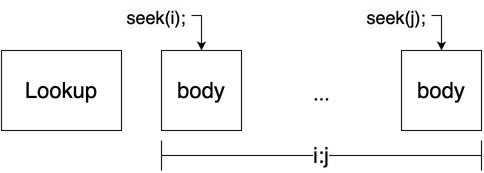
\includegraphics[scale=0.20]{Looplets-lookup.png}
%     \end{minipage}
%     \vspace{3pt}

%     \begin{minipage}[c]{0.65\linewidth}
%         $\finchrun(body)$: The Run Looplet represents a constant
%         region of an iterator. The body of the run is understood to have one
%         less dimension than the lookup itself, as all of the bodies are
%         identical.
%     \end{minipage}%
%     \begin{minipage}[c]{0.35\linewidth}
%         \centering
%         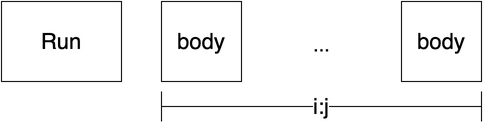
\includegraphics[scale=0.20]{Looplets-run.png}
%     \end{minipage}
%     \vspace{3pt}

%     \begin{minipage}[c]{0.65\linewidth}
%         $\finchphase(c:d, body)$: The Phase Looplet represents a
%         restriction of the range on which a loop should execute, and allows us
%         to succinctly express the ranges on which children of compound looplets
%         are defined.
%     \end{minipage}%
%     \begin{minipage}[c]{0.35\linewidth}
%         \centering
%         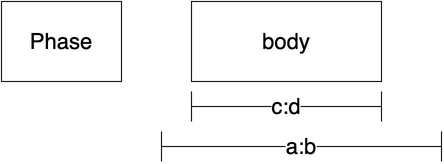
\includegraphics[scale=0.20]{Looplets-phase.png}
%     \end{minipage}
%     \vspace{3pt}

%     \begin{minipage}[c]{0.65\linewidth}
%         $\finchswitch(cond, head, tail)$: The Switch Looplet allows
%         us to specialize the body of a looplet based on a condition, evaluated
%         in the embedding context. If the condition is true, we use `head`,
%         otherwise we use `tail`. Switch has a high lowering priority so we can
%         see what's inside of it and lower that appropriately. This also lifts
%         the condition as high as possible into the loop nest. The condition is
%         assumed to evaluate to a boolean.
%     \end{minipage}%
%     \begin{minipage}[c]{0.35\linewidth}
%         \centering
%         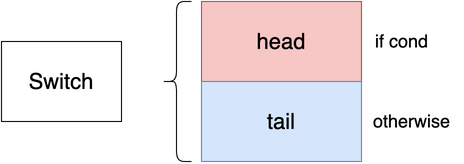
\includegraphics[scale=0.20]{Looplets-switch.png}
%     \end{minipage}
%     \vspace{3pt}

%     \begin{minipage}[c]{0.65\linewidth}
%         $\finchthunk(preamble, body, epilogue)$: The Thunk Looplet
%         allows us to cache certain computations in the state under which the
%         body will execute. This is useful for computing and caching the results
%         of expensive computations.
%     \end{minipage}%
%     \begin{minipage}[c]{0.35\linewidth}
%         \centering
%         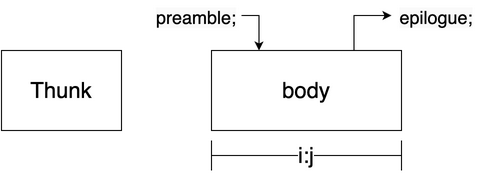
\includegraphics[scale=0.20]{Looplets-thunk.png}
%     \end{minipage}
%     \vspace{3pt}

%     \begin{minipage}[c]{0.65\linewidth}
%         $\finchsequence(head, tail)$: The Sequence looplet represents the
%         concatenation of two looplets. Both arguments must be phase looplets, and
%         are assumed to be nonoverlapping, covering, and in order.
%     \end{minipage}%
%     \begin{minipage}[c]{0.35\linewidth}
%         \centering
%         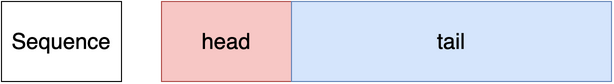
\includegraphics[scale=0.20]{Looplets-sequence.png}
%     \end{minipage}
%     \vspace{3pt}

%     \begin{minipage}[c]{0.65\linewidth}
%         $\finchspike(body, tail)$ The Spike Looplet represents a run
%         followed by a single value. In this paper, Spike will be considered a
%         shorthand for $\finchsequence(\finchphase(i:j-1, \finchrun(body)),
%         \finchphase(j:j, \finchrun(tail)))$.  In the Finch compiler, spikes are
%         handled with special care, since they are an opportunity to align the
%         final run to the end of the root loop extent, without using any special
%         bounds inference.
%     \end{minipage}%
%     \begin{minipage}[c]{0.35\linewidth}
%         \centering
%         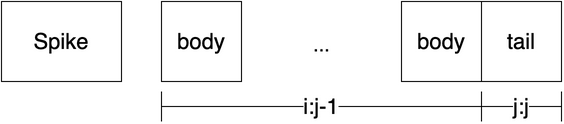
\includegraphics[scale=0.20]{Looplets-spike.png}
%     \end{minipage}
%     \vspace{3pt}

%     \begin{minipage}[c]{0.65\linewidth}
%         $\finchstepper([seek], next, body)$ The stepper looplet
%         represents a variable number of looplets, concatenated. Since our
%         looplets may be skipped over due to conditions or various rewrites, the
%         $seek$ function allows us to fast-forward the state to the start of the
%         root loop extent when it comes time to lower the stepper. The $next$
%         function advances the state to the next iteration of the stepper. 
%     \end{minipage}%
%     \begin{minipage}[c]{0.35\linewidth}
%         \centering
%         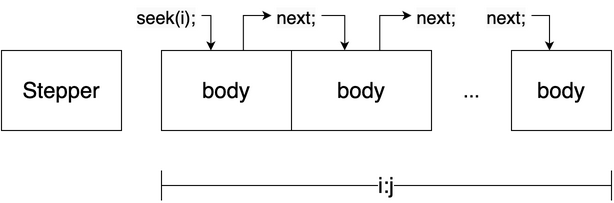
\includegraphics[scale=0.20]{Looplets-stepper.png}
%     \end{minipage}
%     \caption{The looplet language, as understood in a correct execution of a Finch program.}
%     \vspace{-8pt}
% \end{figure}


\begin{figure}[ht]
\footnotesize
\begin{tabular} {|p{0.65\linewidth}|c|} 
    \hline
    $\finchlookup(seek, body)$: The Lookup Looplet represents a randomly accessible region of an iterator. The body of the lookup is understood to have one less dimension than the lookup itself, as we have already ``looked up'' that index in the tensor by the time we reach the body. \texttt{seek(i)} is a function that updates state to the given index.
    &
    \raisebox{-\totalheight}{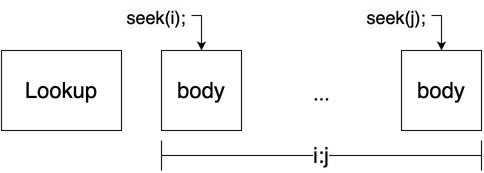
\includegraphics[scale=0.20]{Looplets-lookup.png}}
    \\
    \hline
    $\finchrun(body)$: The Run Looplet represents a constant region of an iterator. The body of the run is understood to have one less dimension than the lookup itself, as all of the bodies are identical.
        &
    \raisebox{-\totalheight}{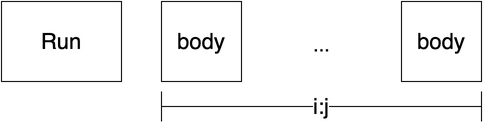
\includegraphics[scale=0.20]{Looplets-run.png}}
    \\ 
    \hline
    $\finchphase(c:d, body)$: The Phase Looplet represents a restriction of the range on which a loop should execute, and allows us to succinctly express the ranges on which children of compound looplets are defined.
    &
    \raisebox{-\totalheight}{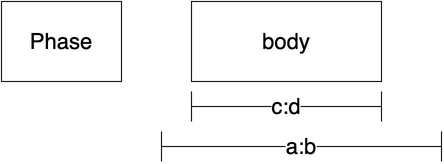
\includegraphics[scale=0.20]{Looplets-phase.png}}
    \\ 
    \hline
    $\finchswitch(cond, head, tail)$: The Switch Looplet allows us to specialize the body of a looplet based on a condition, evaluated in the embedding context. If the condition is true, we use `head`, otherwise we use `tail`. Switch has a high lowering priority so we can see what's inside of it and lower that appropriately. This also lifts the condition as high as possible into the loop nest. The condition is assumed to evaluate to a boolean.
    &
    \raisebox{-\totalheight}{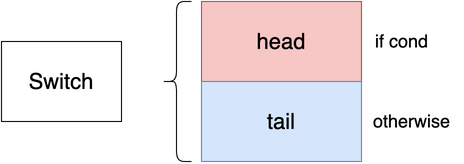
\includegraphics[scale=0.20]{Looplets-switch.png}}
    \\ 
    \hline
    $\finchthunk(preamble, body, epilogue)$: The Thunk Looplet allows us to cache certain computations in the state under which the body will execute. This is useful for computing and caching the results of expensive computations.
    &
    \raisebox{-\totalheight}{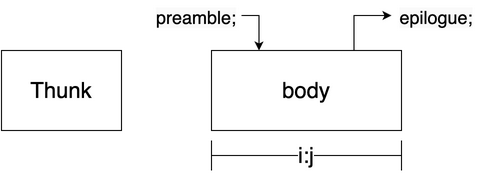
\includegraphics[scale=0.20]{Looplets-thunk.png}}
    \\ 
    \hline
    $\finchsequence(head, tail)$: The Sequence looplet represents the concatenation of two looplets. Both arguments must be phase looplets, and are assumed to be nonoverlapping, covering, and in order.
    &
    \raisebox{-\totalheight}{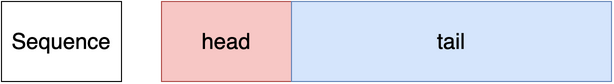
\includegraphics[scale=0.20]{Looplets-sequence.png}}
    \\ 
    \hline
    $\finchspike(body, tail)$: The Spike Looplet represents a run followed by a single value. In this paper, Spike will be considered a shorthand for $\finchsequence(\finchphase(i:j-1, \finchrun(body)), \finchphase(j:j, \finchrun(tail)))$.  In the Finch compiler, spikes are handled with special care, since they are an opportunity to align the final run to the end of the root loop extent, without using any special bounds inference.
    &
    \raisebox{-\totalheight}{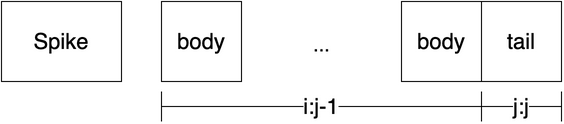
\includegraphics[scale=0.20]{Looplets-spike.png}}
    \\ 
    \hline
    $\finchstepper([seek], next, body)$: The stepper looplet represents a variable number of looplets, concatenated. Since our looplets may be skipped over due to conditions or various rewrites, the $seek$ function allows us to fast-forward the state to the start of the root loop extent when it comes time to lower the stepper. The $next$ function advances the state to the next iteration of the stepper. 
    &
    \raisebox{-\totalheight}{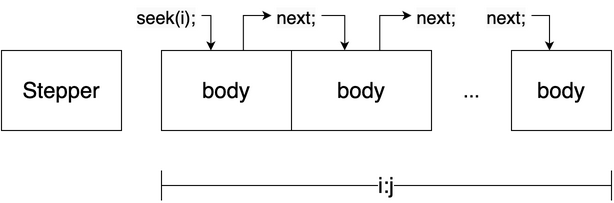
\includegraphics[scale=0.20]{Looplets-stepper.png}}
    \\
    \hline
    \end{tabular}
\vspace{-8pt}
\caption{The looplet language, as understood in a correct execution of a Finch program.}
\end{figure}
\section{Bridging Looplets and Finch: The Tensor Interface}

%
The Finch language provides descriptions of computations that iterate over a subset of a regular grid that is lexicographically ordered.
%
At this point, the reader might believe that compilation of a Finch program simply involves simply replacing for loops over a range with for loops over iterators, but Finch programs and data structures are sufficiently flexible that this impossible.
%
First, the Finch language interacts with multi-dimensional tensors whereas the Looplet abstraction is best suited towards iterators over a single dimension.
%
We require a bridge between the single dimensional iterators created from looplets and the mutli-dimensional abstractions common to tensor compilers.
%
Second, since the iteration order of a Finch program might not match that of a data structure (a discordant traversal), different iterators need to be requested for the same data depending on the traversal order of the program.
%
So we require a bridge that can provide different iteration orders depending on the context.
%
Third, since Finch programs can read and write to the same data, multi-dimensional tensors need to provide iterators for reading and writing as well as machinery to manage transition between these states.


To build our bridge, we embrace a set of abstractions: level formats/Fiber Trees, iteration context dependent instantiation of iterators, and tensor life cycles.
%
Our first abstraction mostly already exists in the literature: a manner of specifying a data structure for a multi-dimensional tensor out of data structures for single dimensional tensors~\cite{sze2017efficient,chou2022compilation, chou2018format}.
%
We recapitulate the essential details here.
%
Our next two abstractions add to to the first by providing a mechanism to use data structures generated by the first abstraction in a greater variety of contexts while maintaining per-dimension encapsulation of array data structures.
%
We introduce an interface to instatiate iterators in a variety of contexts in our programs and we introduce the lifecycle interface to manage when we read and write to multi-dimensional iterators.
%
These interfaces add to the level abstraction, expanding the types of data that they can express via mapping to looplets and expanding the contexts in which they can be used.
%
Previous efforts to compile a greater variety of sparse array programs left these bridges untouched ~\cite{henry_compilation_2021, won2023unified, senanayake2020sparse}.

%What needs to be said about the tensors? It's basically a few main points:
%1. (DONE) What is the level abstraction 
%2. (Done) We have identified 8 key level structures to represent most combinations of runs or pinpoints.
%2. a. beautiful figure with datas as rows of larger structures
%2. b. How do we write to each of these, in order? Randomly? random access? several important datastructures that show up along the way.
%3. What is "Unfurling"? and how does it help us represent each structure? refer to looplet decompositions of each case in the earlier figure
%4. What are lifecycles? How do lifecycles help us keep sane? Why are they necessary for correctness?

\subsection{Level Abstraction}
Fiber-tree style tensor abstractions have been the subject of extensive study
\cite{sze2017efficient, chou2022compilation, chou2018format}.  The underlying
idea is to represent a multi-dimensional tensor as a nested vector
datastructure, where each level of the nesting corresponds to a dimension of the
tensor. Thus, a matrix would be represented as a vector of vectors. This kind of
abstraction lends itself to representing sparse tensors if we vary the type of
vector used at each level in a tree. Thus, a sparse matrix might be represented
as a dense vector of sparse vectors. The vector of subtensors in this
abstraction is referred to as a \textbf{fiber}. Prior fiber-tree representations
focus on sparsity (where only the nonzero elements are represented) and treat
sparse vectors as sets of represented points. Since our fiber-tree
represesentation must handle other kinds of structure, such as diagonal,
repeated, or constant values, we instead view each fiber as a mapping from
indices into a space of subfibers.

%From the docs:
%Finch represents tensors hierarchically in a tree, where each node in the tree is a vector of subtensors and the leaves are the elements. Thus, a matrix is analogous to a vector of vectors, and a 3-tensor is analogous to a vector of vectors of vectors. The vectors at each level of the tensor all have the same structure, which can be selected by the user.
%In a Finch tensor tree, the child of each node is selected by an array index. All of the children at the same level will use the same format and share the same storage. Finch is column major, so in an expression A[i_1, ..., i_N], the rightmost dimension i_N corresponds to the root level of the tree, and the leftmost dimension i_1 corresponds to the leaf level.
%We refer to a node in the tree as a subfiber. All of the nodes at the same level are stored in the same datastructure, and disambiguated by an integer position. in the above example, there are three levels: the rootmost level contains only one subfiber, the root. The middle level has 3 subfibers, one for each column. The leafmost level has 12 subfibers, one for each element of the array. For example, the first level is A_fbr.lvl, and we can represent it's third position as SubFiber(A_fbr.lvl.lvl, 3). The second level is A_fbr.lvl.lvl, and we can access it's 9th position as SubFiber(A_fbr.lvl.lvl.lvl, 9). For instructional purposes, you can use parentheses to call a subfiber on an index to select among children of a subfiber.
%When we print the tree in text, positions are numbered from top to bottom. However, if we visualize our tree with the root at the top, positions range from left to right:
%Dense Format Index Tree
%Because our array is sparse, (mostly zero, or another fill value), it would be more efficient to store only the nonzero values. In Finch, each level is represented with a different format. A sparse level only stores non-fill values. This time, we'll use a tensor constructor with sl (for "SparseList of nonzeros") instead of d (for "Dense"):
%CSC Format Index Tree
%Our Dense(SparseList(Element(0.0))) format is also known as "CSC" and is equivalent to SparseMatrixCSC. The Tensor function will perform a zero-cost copy between Finch fibers and sparse matrices, when available. CSC is an excellent general-purpose representation when we expect most of the columns to have a few nonzeros. However, when most of the columns are entirely fill (a situation known as hypersparsity), it is better to compress the root level as well:
%DCSC Format Index Tree
%Here we see that the entirely zero column has also been compressed. The SparseList(SparseList(Element(0.0))) format is also known as "DCSC".
%The COO format is compact and straightforward, but doesn't support random access. For random access, one should use the SparseHash format. A full listing of supported formats is described after a rough description of shared common internals of level, relating to types and storage.
%All levels have a postype, typically denoted as Tp in the constructors, used for internal pointer types but accessible by the function:
%postype(lvl)

Instead of storing the data for each subfiber separately, most sparse tensor
formats such as CSR, DCSR, and COO usually store the data for all fibers in a
level contiguously. In this way, we can think of a level as a bulk allocator for
fibers. Continuing the analogy, we can think of each fiber as being
disambiguated by a \textbf{position}, or an index into the bulk pool of
subfibers. The mapping $f$ from indices to subfibers is thus a mapping from an
index and a position in a level to a subposition in a sublevel.
Figure~\ref{fig:levelsvsfibers} shows a simple example of a level as a pool of fibers.

When we need to refer to a particular fiber at position $p$ in the level $l$, we
may write $fiber(l, p)$. Note that the formation of fibers from levels is lazy,
and the data underlying each fiber is managed entirely by the level, so the
level may choose to overlap the storage between different fibers. Thus, the only
unique data associated with $fiber(l, p)$ is the position $p$.

\begin{figure}
    \centering
    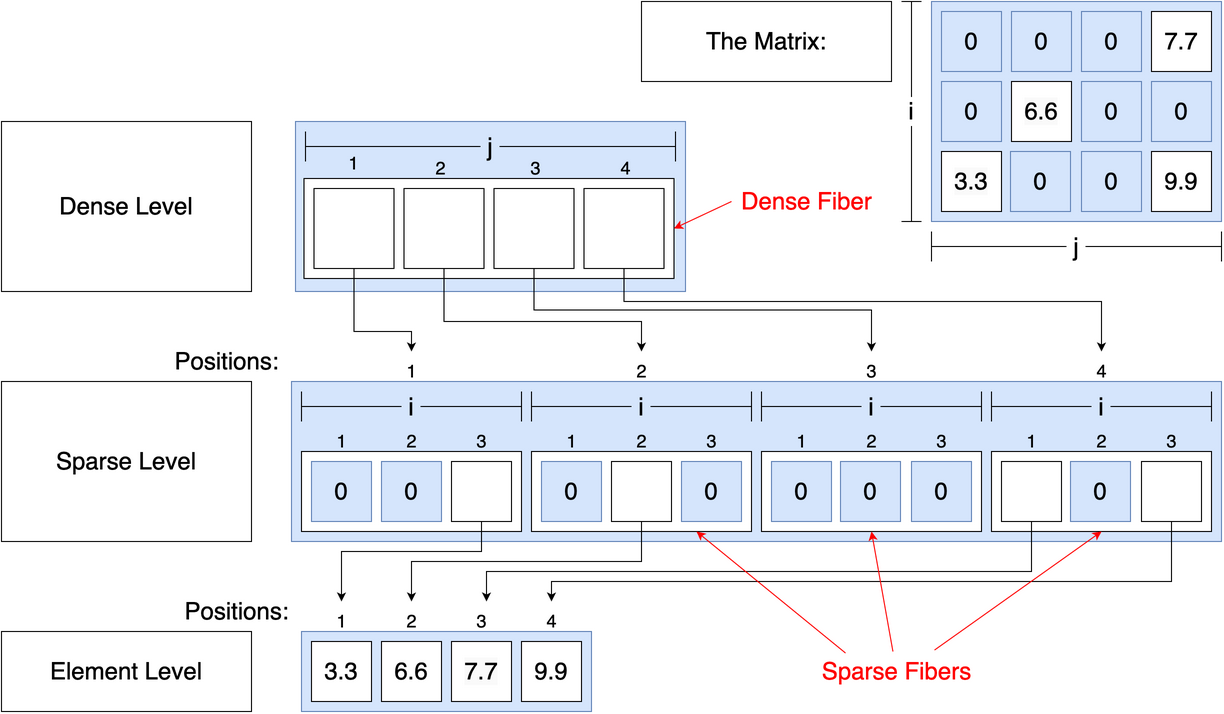
\includegraphics[width=0.45\linewidth]{LevelsVsFibers-matrix.png}\hfill%
    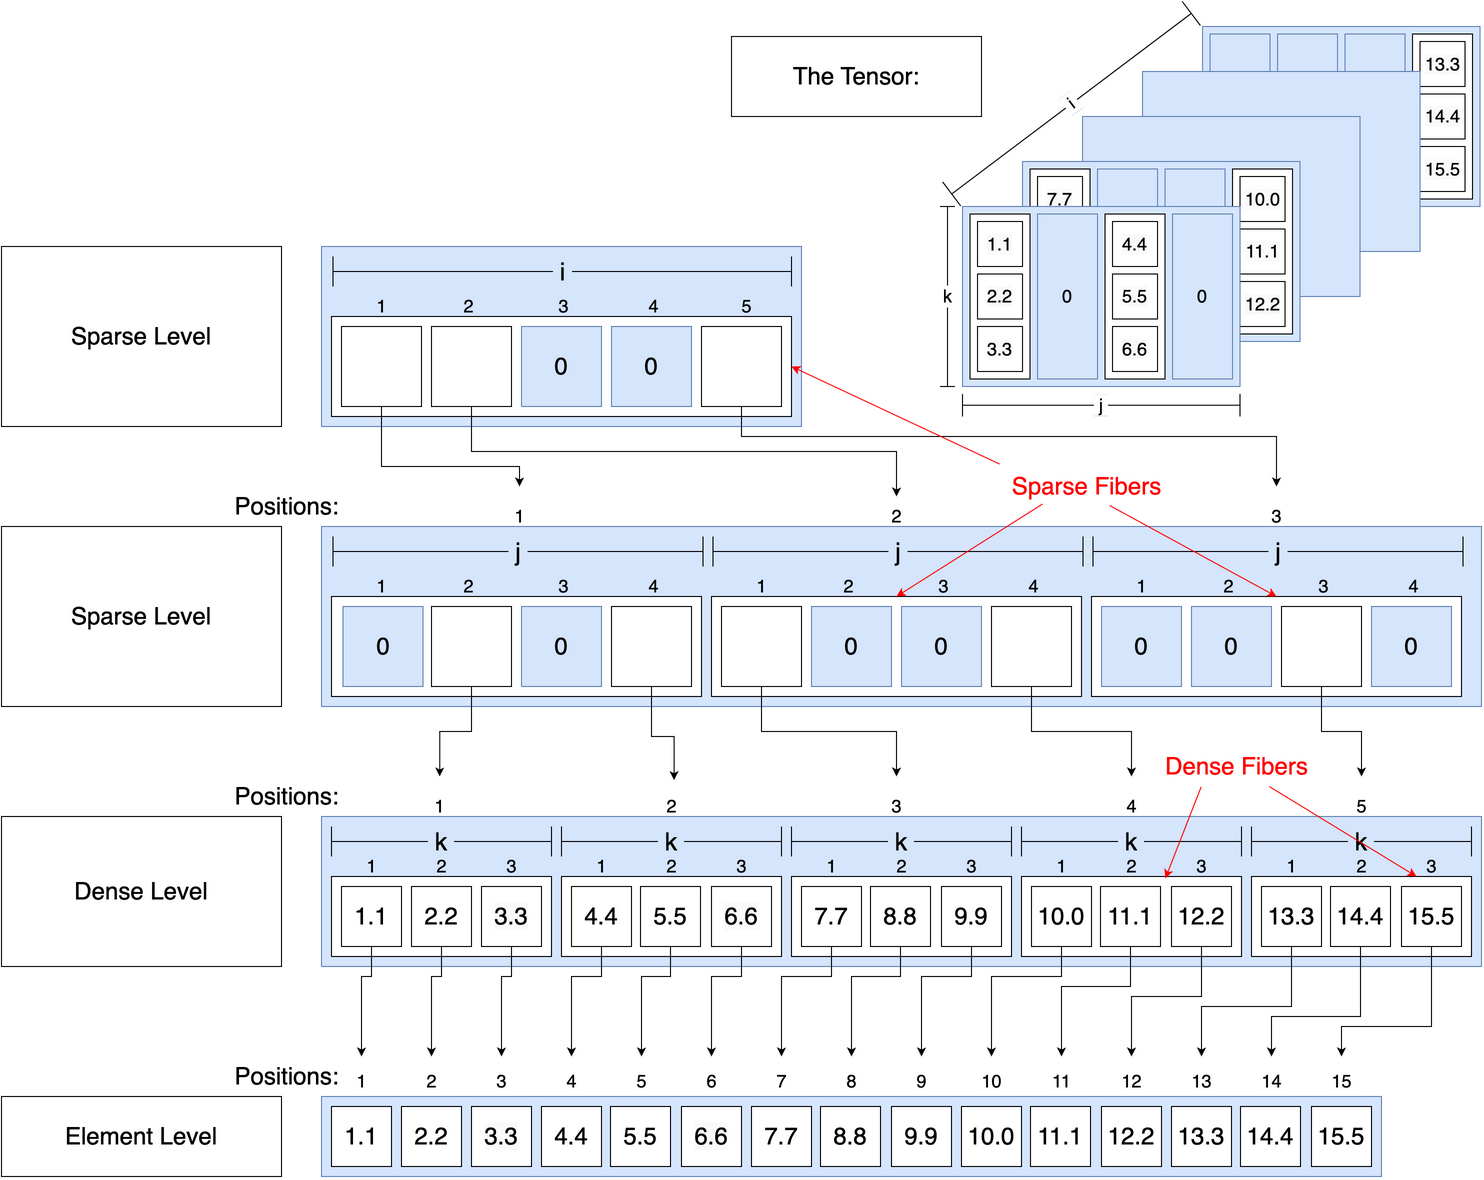
\includegraphics[width=0.5\linewidth]{LevelsVsFibers-tensor.png}
    \caption{Levels and fiber tree representations of a sparse matrix and a sparse tensor. On left, a matrix is represented in a fibertree corresponding to CSC format, with a dense outer level and a sparse inner level. On right, a tensor is represented in a fibertree with two sparse outer levels, and a dense inner level. Note that the element levels in this case form the leaves of the tree.}
    \label{fig:levelsvsfibers}
\end{figure}

\subsection{The 8 Key Level Structures}
    \begin{wrapfigure}{r}{.35\textwidth}
        \centering
        \scriptsize
        \begin{tabular}{|c|c|c|c|l|}
            \hline
            \rothead{Sparse} & \rothead{Blocked} & \rothead{Runs} & \rothead{Singletons} & \begin{tabular}{@{}l@{}}\textbf{Corresponding} \\ \textbf{Format}\end{tabular} \\
            \hline
             &  &  &  & Dense \\
            \hline
             &  & \checkmark &  & DenseRLE \\
            \hline
            \checkmark &  &  &  & Sparse \\
            \hline
            \checkmark &  &  & \checkmark & SparsePinpoint \\
            \hline
            \checkmark &  & \checkmark &  & SparseRLE \\
            \hline
            \checkmark &  & \checkmark & \checkmark & SparseInterval \\
            \hline
            \checkmark & \checkmark &  &  & SparseVBL \\
            \hline
            \checkmark & \checkmark &  & \checkmark & SparseBand \\
            \hline
        \end{tabular}
        \caption{All combinations of relevant structural properties and their
        corresponding formats.  Note that blocks and runs need not be considered
        together because we must store a run length for each run, and so there
        isn't a significant storage benefit to combining them. Blocks and
        singletons only make sense in the contex of sparsity, so we don't
        consider them together either. We omit such combinations
        from the exhaustive table.}
        \label{tab:TypesOfStructure}
    \end{wrapfigure}
    The main benefits of specializing to structure come from the following properties of the data:
    \begin{enumerate}
        \item[Sparsity] Sparse data is data that is mostly zero, or some other
        fill value. When we specialize on this data, we can use annihilation ($x
        * 0 = 0$), identity ($x * 1 = 1$), or other constant propagation
        properties ($ifelse(false, x, y) = y$) to simplify the computation and avoid
        redundant work.
        
        \item[Blocks] Blocked data is a subset of sparse data where the nonzeros
        are clustered and occur adjacent to one another. This provides us with
        two opportunities: We can avoid storing the locations of the nonzeros
        individually, and we can use more efficient randomly accessible
        iterators within the block. \cite{im_optimizing_2001, vuduc_performance_2002, ahrens_looplets_2023}.

        \item[Runs] Runs of repeated values may occur in dense or sparse code,
        cutting down on storage and allowing us to use integration rules such as 
        \mintinline{julia}{for i = 1:n; s += x end} $\rightarrow$
        \mintinline{julia}{s += n * x} or code motion to lift operations out of loops \cite{donenfeld_unified_2022,ahrens_looplets_2023}.

        \item[Singletons] When we have only one non-fill region in sparse data,
        we can avoid a loop entirely and reduce the complexity of iteration \cite{ghorbani2023compiling, ahrens_looplets_2023}.
    \end{enumerate}

    In Finch, we have identified 8 key level structures that can represent all
    of the relevant combinations of these properties, summarized in Table
    \ref{tab:TypesOfStructure}. We examine each structure in turn, describing
    some of the key properties and potential use cases of each. In this sense,
    the structures we consider are exhaustive. We can represent a wide variety
    of hierarchical tensor structures by combining these level structures in a
    tree, as shown in Figure~\ref{fig:structuraldiversity}.

    \begin{figure}
        \centering
        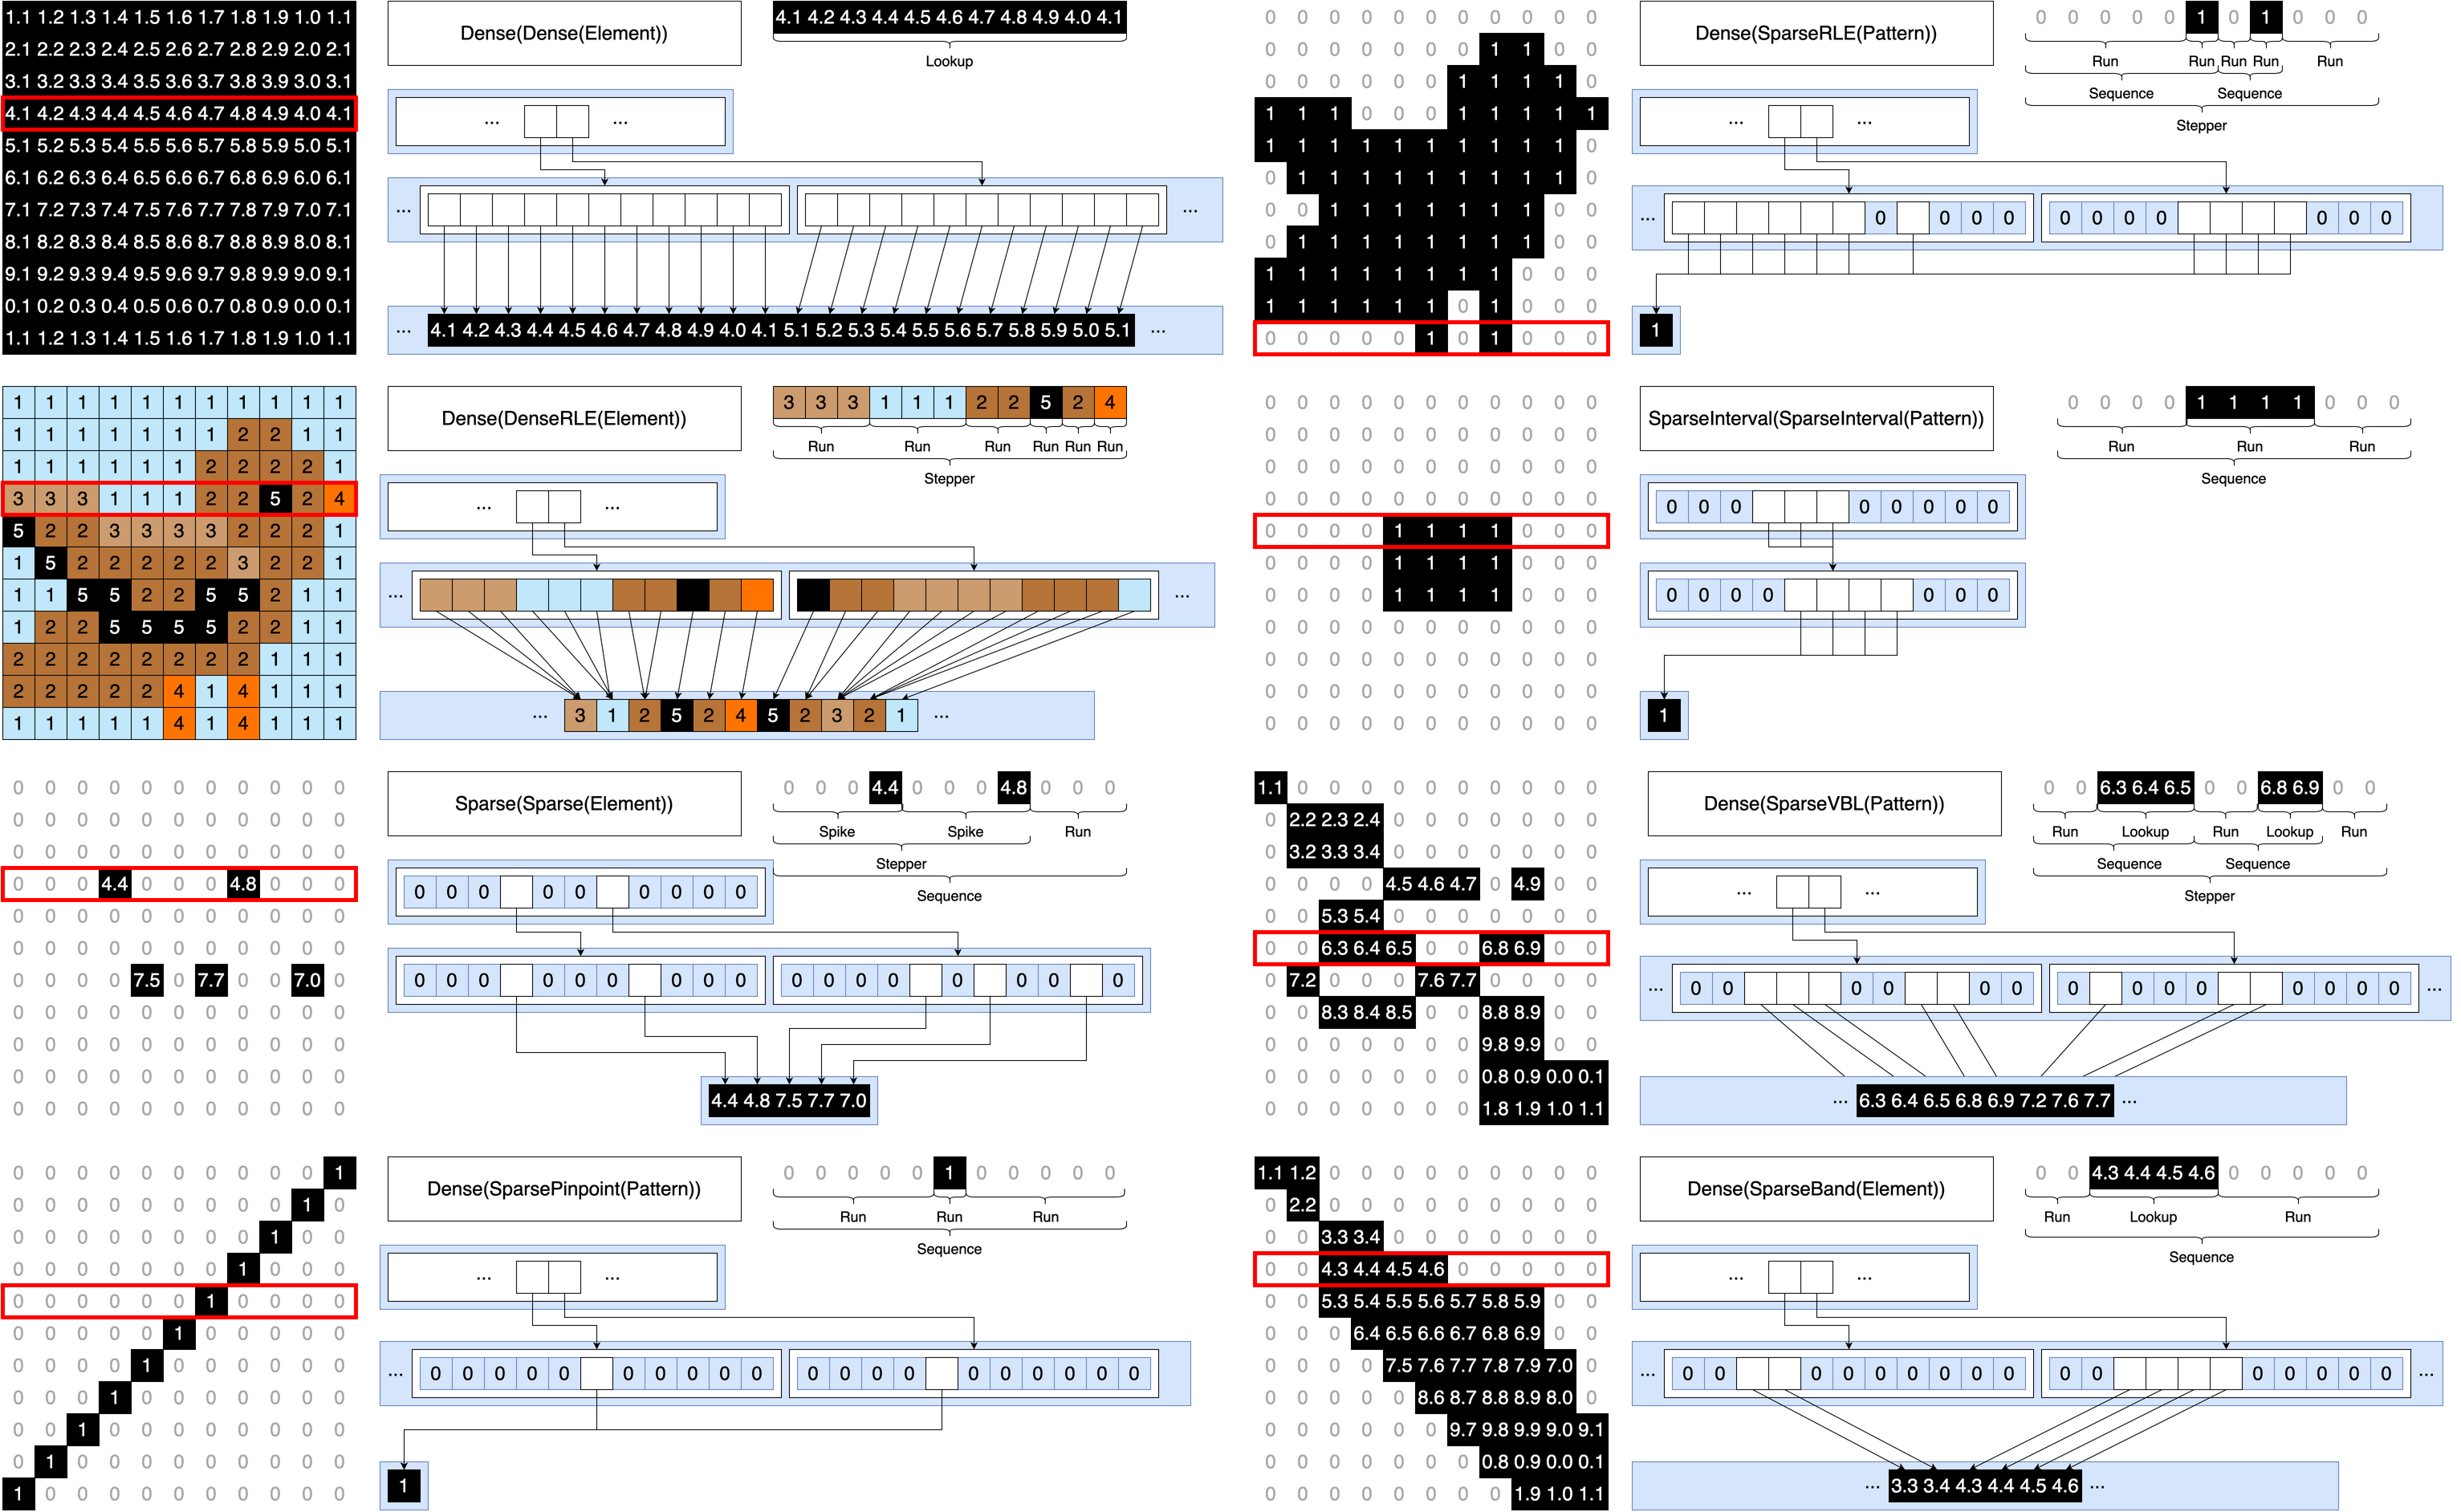
\includegraphics[width=\linewidth]{Structures.png}\hfill%
        \caption{Several examples of matrix structures represented using the
        level structures identified in Table~\ref{tab:TypesOfStructure}.
        Comparing this figure to \cite[Figure 3]{ahrens_looplets_2023}, we see
        that a level-by-level structural decomposition is diagrammed together
        with the Looplets.}
        \label{fig:structuraldiversity}
    \end{figure}

\subsection{Tensor Lifecycle, Declare, Freeze, Thaw, Unfurl}

Our simplified view of a level is enabled by our use of looplets to represent
the structure within each fiber. In fact, our level interface requires only 5
highly general operations, described below.

The first three of these functions, declare, freeze, and thaw, have to do with
managing when tensors can be assumed mutable or immutable. As we use Looplets to
represent iteration over a tensor, we must restrict the mutability of tensors
while we iterate over them. For example, if a tensor declares it has a constant
region from $i = 2:5$, but some other part of the computation modifies the
tensor at $i = 3$, this would result in incorrect behavior. It is much easier to
write correct Looplet code if we can assume that the tensor is immutable while
we are reading from it. Thus, we introduce the notion that a tensor can be in
read-only mode or update-only mode.  In read-only mode, the tensor may only
appear in the right-hand side of assignments. In update-only mode, the tensor
may only appear in the left-hand side of an assignment, either being overwritten
or incremented by some operator.  We can switch between these modes using freeze
and thaw functions. The declare function is used to allocate a tensor,
initialize it to some specified size and value, and leave it in update-only
mode. 

The unfurl function is used to manage iteration over a subfiber. At the point
when it comes time to iterate over a tensor, be in on the left or right hand
side of an assignment, we call the unfurl function to precompute whatever state
and datastructures are necessary to return a looplet nest that would iterate
over that level of a tensor. The unfurl function is called directly before
iterating over the corresponding loop, so it has access to any state variables introduced
by freezing or thawing the tensor.

Our view of a level as a fiber allocator implies an allocation function
$assemble(tns, pos_{start}:pos_{stop})$, which allocates fibers at positions
$pos_{start}:pos_{stop}$ in the level. We don't specify a de-allocation
function, instead relying on initialization to reset the fiber if it needs to be
reused. While all of the previous functions are used to manage the lifecycle and
iteration over a general tensor, the assemble function is quite specific to the
level abstraction, and the notion of positions within sublevels. Note: it was an
intentional choice to hold the parent level responsible for managing the
data of the sublevels, which positions they allocate, etc. This allows the parent
level to reuse allocation logic from internal index datastructures. For example,
a sparse level might use a list of indices to store which nonzeros are present,
and when it comes time to resize that list, it could also call assemble to resize the
sublevel, reducing the number of branches in the code. The assemble function
lends itself particularly to a "vector doubling" allocation approach, which we
have found to be effective and flexible when managing the allocation
of sparse left hand sides. This benefit is made clear in our evaluation section,
where we see that prior systems like TACO do not support all possible loop
orderings and format combinations for sparse matrix multiply because they do
not have a flexible enough allocation strategy, instead using a two-phase approach
which requires computing a complicated closed-form kernel to iterate over the
data twice to determine the number of required output nonzeros.

\begin{figure}
    \raggedright
\paragraph{$declare(lvl, init, dims...)$} Declares the level to hold subtensors
of size $dims$ and an initial value of $init$. Requires the level to be in
read-only mode.
\paragraph{$freeze(lvl)$} Finalizes the updates in the level, and readies the
level for reading. Requires the level to be in update-only mode.
\paragraph{$thaw(lvl)$} Prepares the level to accept updates. Requires the level
to be in read-only mode.
\paragraph{$unfurl(fiber(lvl, pos), ext, mode)$} Unfurls the fiber at position
$pos$ in the level $lvl$ over the extent $ext$. When $mode = \finchread$,
returns a looplet nest over the values in the read-only fiber.  When $mode =
\finchupdate$, returns a looplet nest over mutable subfibers in the update-only
fiber. Often, skipping over mutable locations allows the level to know which
locations must be stored. Additionally, a dirty bit may be used to communicate
whether the mutable subfiber has been written to, which allows the parent fiber
to know whether the subfiber must be stored explicitly.
\paragraph{$assemble(lvl, pos_{start}, pos_{stop})$} Allocates subfibers in the
level from positions $pos_{start}$ to $pos_{stop}$. Usually, this function is
only ever called on unassembled positions, but some levels (such as dense levels
or bytemaps) may support reassembly.
\caption{The five functions that define a level.}
\end{figure}

\subsection{Level Formats}
Having described the 8 basic level structures and the functions that define a
level format, we can describe the concrete level formats supported by Finch,
some of the challenges in their implementation, and how we overcome them. Note
that these formats are not meant to be exhaustive; we will later give
recommendations for additional level formats to be implemented and explain how
users can also add their own custom formats. Note that all of the levels below store their shape and a sublevel.

\begin{enumerate}
\item[Dense]
    The dense format is the simplest format, and simply maps $fiber(l, p)[i]
    \rightarrow fiber(l.lvl, p * l.shape + i)$. This format is used to store dense data,
    and is often a convenient format for the root level of a tensor. Because
    of its simplicity, freezing and thawing the level are no-ops.
\item[DenseRLE]
    The DenseRLE format is used to represent runs of repeated values. Notice
    that a challenge arises when trying to write to a level with runs: it is
    difficult to merge duplicate runs. Such a scenario might arise when merging
    runs of subfibers of length 3, representing colors in an image.  Ideally, we
    would be able to detect duplicate subfibers and merge them on the fly, but
    we cannot determine which subfibers are equal because we cannot read them
    while the sublevel is in update-only mode. Instead, we merge the duplicates
    during the freeze phase. We $freeze$ the main sublevel, $declare$ a separate
    sublevel as a buffer to store the deduplicated subfibers, and we can then
    compare each of the subfibers in the main level, copying the deduplicated
    subfibers into the buffer:
    \begin{enumerate}
        \item[$right$] A vector of indices corresponding to the end of each run in the level
        \item[$ptr$] A vector of delimiters such that $right[ptr[p]:ptr[p+1] - 1]$ is the set of delimiters in the subfiber at position $p$.
        \item[$buf$] A duplicate sublevel, used to store deduplicated subfibers during $freeze$.
    \end{enumerate}
\item[SparseList]
    The sparse list format is the simplest sparse format, and is used to
    construct the popular CSR, CSC, DCSR, DCSC, and CSF formats. The sparse list
    format consists of the following fields:
    \begin{enumerate}
        \item[$idx$] A vector of nonzero indices in the level
        \item[$ptr$] A vector of delimiters such that $idx[ptr[p]:ptr[p+1] - 1]$ is the set of nonzero indices in the subfiber at position $p$.
    \end{enumerate}
    All of Finch's sparse formats use a dirty bit during writing to determine
    whether the sublevel has been modified from it's default fill value and
    thus, whether it needs to be stored.
\item[SparsePinpoint]
    Because the SparsePinpoint format will only ever store one nonzero in each subfiber,
    we do not need the $ptr$ field.
    \begin{enumerate}
        \item[$idx$] A vector of nonzero indices in the level, one for each subfiber
    \end{enumerate}
\item[SparseRLE]
    Similar to the DenseRLE level, but because the runs are stored on top of a background of fill values, we must also store the start of each run.
    \begin{enumerate}
        \item[$left$] A vector of indices corresponding to the beginning of each run in the level
        \item[$right$] A vector of indices corresponding to the end of each run in the level
        \item[$ptr$] A vector of delimiters such that $left[ptr[p]:ptr[p+1] - 1]$ and $right[ptr[p]:ptr[p+1] - 1]$ are the set of delimiters in the subfiber at position $p$.
        \item[$buf$] A duplicate sublevel, used to store deduplicated subfibers during $freeze$.
    \end{enumerate}
\item[SparseInterval]
    Similar to the SparseRLE level, but $ptr$ is redundant because we only store
    one run. We also don't bother with deduplication here as we cannot store any
    intermediate results with duplicates.
    \begin{enumerate}
        \item[$left$] A vector of indices corresponding to the beginning of each run in the level
        \item[$right$] A vector of indices corresponding to the end of each run in the level
    \end{enumerate}
\item[SparseVBL]
    The SparseVBL format is used to represent blocked data. The format consists
    of the following fields:
    \begin{enumerate}
        \item[$idx$] A vector of indices at the end of each nonzero block in the level
        \item[$ptr$] A vector of delimiters such that $idx[ptr[p]:ptr[p+1] - 1]$ is the set of block terminals in the subfiber at position $p$.
        \item[$ofs$] A vector of delimiters such that $ofs[ptr[p] + q]:ofs[ptr[p] + q + 1] - 1$ are the subpositions of block $q$ in subfiber $p$.
    \end{enumerate}
\item[SparseBand]
    Like SparseVBL, but only one block is stored in each subfiber.
        \item[$idx$] The index at the end of the block in the level
        \item[$ofs$] A vector of delimiters such that $ofs[p]:ofs[p + 1] - 1$ are the subpositions of the block in subfiber $p$.
\end{enumerate}

\help{we need also to talk about pattern and element}

\subsection{Flexible Level Formats}
The levels we described in the previous section are all oriented towards bulk,
sequential creation of formats. However, when users want to be able to write out
of order (which is a common requirement arising from loop order or from the
problem itself, it occurs in our spgemm algorithms and our histogram example in
the evaluation section), we must use more complicated datastructures like hash
tables and trees to support the random access. Because these datastructures are
more complex and have a higher implementation burden and performance overhead,
we only support random access construction of sparse or dense structures.  We
can use these two more general structures as intermediates to convert to our
more specialized structures later.

\begin{enumerate}
\item[SparseHash]
    The sparse hash format uses a hash table to store the locations of nonzeros,
    and sorts the unique indices for iteration during the freeze phase. This
    allows for efficient random access, but not incremental construction, as the
    freeze phase runs in time proportional to the number of nonzeros in the
    entire level.
    \begin{enumerate}
        \item[$idx$] A vector of nonzero indices in the level
        \item[$ptr$] A vector of delimiters such that $idx[ptr[p]:ptr[p+1] - 1]$ is the set of nonzero indices in the subfiber at position $p$.
        \item[$tbl$] A hash table used for construction of the level.
    \end{enumerate}
\item[SparseBytemap]
    The SparseBytemap format uses a bytemap to store which locations have been
    written to. Unlike the SparseHash format, the bytemap assembles the entire
    space of possible subfibers. This accelerates random access in the format,
    but requires a high memory overhead. Because we don't want to reallocate all
    of the memory in each iteration, the declaration of this format instead
    re-assembles only the dirty locations in the tensor. This format is
    analogous to the default workspace format used by TACO.
    \begin{enumerate}
        \item[$idx$] A vector of nonzero indices in the level
        \item[$ptr$] A vector of delimiters such that $idx[ptr[p]:ptr[p+1] - 1]$ is the set of nonzero indices in the subfiber at position $p$.
        \item[$tbl$] A dense array of booleans used to mark dirty locations in the tensor.
    \end{enumerate}
\end{enumerate}

As future work, we also recommend the implementation of a tree-based format, as
this would enable incremental construction. Currently, the cost of freezing and
thawing is usually proportional to the number of stored fibers, so an operation
that sets a single value in a tensor would be prohibitively expensive (i.e.
$A[3, 4] = 3.14$). We would also recommend supporting SparseRLE as an
intermediate randomly accessible structure, because (unlike blocks or
singletons), runs have asymptotic benefits. However, these cases were not
necessary for our case studies.

\subsection{Scalars}

\subsubsection{Sparse Scalars}
\subsubsection{Early Break Scalars}

\section{The Finch Language}

\subsection{Syntax}

The syntax of Finch is displayed in Figure \ref{fig:syntax}. The Finch syntax
mirrors most imperative languages with for-loops and control flow. Notable
inclusions to the language include \mintinline{julia}{for},
\mintinline{julia}{let}, blocks of code with \mintinline{julia}{if}, and 
the lifecycle functions that let us declare, freeze, and thaw tensors.

Finch uses looplets to lower \mintinline{julia}{for}-loops, though a sparse
program with complicated looplets should produce output tensors with the same
semantic value as a dense program with ordinary for-loops.  We include the
semantics of how looplets are lowered as it affects the structure of the results
and the asymptotic complexity of the program. Some applications view the
structure of tensors as semantically meaningful.

The \mintinline{julia}{let} statement (marked by the \finchdefine AST node)
allows us to define tensor variables and reuse their value in multiple
subexpressions without passing the variable through a tensor. Although it is too
complex in this work to propagate constants through tensors, we can propagate
constants (including 0) through a define statement. This allows the compiler to
build up complicated functions of known operators and infer annihilation
properties through them.It also allows use to eliminate common subexpressions,
or tensor accesses, by reusing a tensor value in multiple places (such as the
symmetric spmv in Figure \ref{fib:spmv_programs}). As another example, in the
following program we don't need to define sparsity and annihilator properties of
$f(a + b) * (a - b)$, as we can derive this from the more basic operators, and
the code only reads from $A$ and $B$ once.
\begin{minted}{julia}
    let a = A[i, j]
        let b = B[i, j]
            C[i, j] = (a + b) * (a - b)
        end
    end
\end{minted}

We allow the use of blocks of code to describe multiple operations. This allows
us to support both multiple outputs and temporary tensors, seen most prominently
in our implementation of gustavson's algorithm for sparse-sparse matrix multiply
and breadth-first-search. Our breadth-first seach also uses an
\mintinline{julia}{if} statement to avoid operating on vertices outside the
frontier. We have found that \mintinline{julia}{if} is particularly useful in
our model for masking to avoid work.

Finally, we add some explicit functions to advance the lifecycle of a tensor.
Note that the user would not typically write \mintinline{julia}{@freeze} or
\mintinline{julia}{@thaw} explicitly as those can be inferred through a separate
pass.

\begin{figure}
\scriptsize
\noindent % This ensures the minipages fill the page width
\begin{minipage}{0.4\linewidth}
\begin{align*}
    \finchliteral(val \in \mathbb{V}) &:= \text{\mintinline{julia}{val}} \\
    \finchvalue(ex \in \mathbb{S}, type \in \mathbb{T}) &:= \text{\mintinline{julia}{ex :: type}} \\
    \finchtensor(name \in \mathbb{S}) &:= \text{\mintinline{julia}{name}} \\
    \finchindex(name \in \mathbb{S}) &:= \text{\mintinline{julia}{name}} \\
    \finchvar(name \in \mathbb{S}) &:= \text{\mintinline{julia}{name}} \\
    \finchextent(a \in E, b \in E) &:= \text{\mintinline{julia}{a : b}} \\
    \finchcall(f \in E, args\ldots \in E) &:= \text{\mintinline{julia}{f(args...)}} \\
    \finchaccess(tns \in T, idxs\ldots \in E) &:= \text{\mintinline{julia}{tns[idxs...]}} \\
    \finchfreeze(tns \in T) &:= \text{\mintinline{julia}{@freeze(tns)}} \\
    \finchthaw(tns \in T) &:= \text{\mintinline{julia}{@thaw(tns)}} \\
    \finchmode(tns \in T) &:= \text{\mintinline{julia}{@mode(tns)}} \\
\end{align*}
\end{minipage}%
\begin{minipage}{0.5\linewidth}
\begin{align*}
    \mathbb{V} &:= \text{the set of all values.} \\
    \mathbb{S} &:= \text{the set of all symbols.} \\
    \mathbb{T} &:= \text{the set of all types.} \\
    I &:= \finchindex \\
    A &:= \finchaccess \\
    V &:= \finchvar \\
    T &:= \finchtensor \\
    E &:= \finchliteral \mid \finchvalue \mid \finchindex \\
        &\quad \mid \finchvar \mid \finchextent \mid \finchcall \mid \finchaccess \\
    S &:= \finchassign \mid \finchloop \mid \finchdefine \\
        &\quad \mid \finchsieve \mid \finchblock \\
\end{align*}
\end{minipage}%
\begin{align*}
    \finchdeclare(tns \in T, init \in E, dims\ldots \in E) &:= \text{\mintinline{julia}{tns .= init(dims...)}} \\
    \finchassign(lhs \in A, op \in E, rhs \in E) &:= \text{\mintinline{julia}{lhs <<op>>= rhs}} \\
    \finchloop(idx \in I, range \in E, body \in S) &:= \text{\mintinline{julia}{for idx = range; body end}} \\
    \finchdefine(var \in V, val \in E, body \in S) &:= \text{\mintinline{julia}{let var = val; body end}} \\
    \finchsieve(cond \in E, body \in S) &:= \text{\mintinline{julia}{if cond; body end}} \\
    \finchblock(bodies\ldots \in S) &:= \text{\mintinline{julia}{begin; bodies... end}}
\end{align*}
\caption{The syntax of the finch language. Note that instead of a classic EBNF
form, we have constrained the classes of subterms on the left hand side to allow
for descriptive names of the arguments. Compare this grammar to the Concrete
Index Notation of TACO \cite[Figure~3]{kjolstad_tensor_2019}, noting the
addition of multiple left hand sides through code blocks, and the explicit
initialization and finalization of tensors.}\label{fig:syntax}
\end{figure}

\subsection{Semantics}

We present a sketch of a small-step operational semantics, showing how to execute a Finch program in a host language.
We break our description of the semantics of Finch into three parts, those
relating to lowering the language itself in Figure~\ref{fig:semantics_core},
those pertaining to the lifecycle of tensors in
Figure~\ref{fig:semantics_lifecycle}, and the semantics of the looplets in
Figure~\ref{fig:semantics_looplets}. Note that in addition to the rules seen
here, we also apply extensive symbolic simplification of the program whenever we
can. In the implementaiton of the language we have heuristics for when to run a
simplification pass, but for the purposes of understanding the semantics of the
language we should understand simplification rules as occuring whenever possible
before continuing to execute the program as normal.

Note that both Looplets and Finch are designed to be embedded into a larger
language, and a separate state variable is introduced for this language.  

\begin{figure}
    \centering
    \footnotesize

    \begin{prooftree}
    \hypo{\langle val, (e, t) \rangle
    \rightarrow val'}
    \infer1[$Define$]{\splitfrac{\langle\finchdefine(var, val, body), (e, t)\rangle}{\rightarrow \langle body, (e[var \mapsto val'], t) \rangle}}
    \end{prooftree}
    \hfill
    \begin{prooftree}
        \hypo{\langle args_i, (e, t) \rangle \Rightarrow vals_i}
        \hypo{\langle f, (e, t) \rangle \Rightarrow g}
        \infer2[$Call$]{\langle\finchcall(f, args...), (e, t)\rangle \rightarrow \llangle g(vals...), t \rrangle}
    \end{prooftree}
    \vspace{6pt}

    \begin{prooftree}
        \hypo{}
        \infer1[$Literal$]{\langle\finchliteral(val), (e, t)\rangle \rightarrow val}
    \end{prooftree}
    \hfill
    \begin{prooftree}
        \hypo{}
        \infer1[$Value$]{\langle\finchvalue(ex, type), (e, t)\rangle \Rightarrow \llangle ex, t \rrangle}
    \end{prooftree}
    \vspace{6pt}

    \begin{prooftree}
        \infer0[$Variable$]{\splitfrac{\langle\finchvar(name), (e, t)\rangle}{\rightarrow e(\finchvar(name))}}
    \end{prooftree}
    \hfill
    \begin{prooftree}
        \infer0[$Index$]{\splitfrac{\langle\finchindex(name), (e, t)\rangle}{\rightarrow e(\finchindex(name))}}
    \end{prooftree}
    \vspace{6pt}

    \begin{prooftree}
        \hypo{\langle head, s_1 \rangle \rightarrow s_2}
        \infer1[$BlockHead$]{\langle\finchblock(head, tail...), s_1 \rangle \rightarrow \langle \finchblock(tail...), s_2 \rangle}
    \end{prooftree}
    \hfill
    \begin{prooftree}
        \infer0[$EmptyBlock$]{\langle\finchblock(), s\rangle \rightarrow s}
    \end{prooftree}
    \vspace{6pt}

    \begin{prooftree}
        \hypo{\langle cond, s \rangle \Rightarrow true}
        \infer1[$SieveTrue$]{\langle\finchsieve(cond, body), s\rangle \rightarrow \langle body, s \rangle}
    \end{prooftree}
    \hfill
    \begin{prooftree}
        \hypo{\langle cond, s \rangle \Rightarrow false}
        \infer1[$SieveFalse$]{\langle\finchsieve(cond, body), s\rangle \rightarrow s}
    \end{prooftree}
    \vspace{6pt}
    
    \begin{prooftree}  
    \hypo{s = (e, t)}
    \hypo{e(tns) = tns'}
    \hypo{\langle init, s \rangle \Rightarrow init'}
    \hypo{\forall i \langle init, dims_i \rangle \Rightarrow dims'_i}
    \infer4[$Declare$]{\langle \finchdeclare(tns, init, dims), (e, t)\rangle \rightarrow (e [\finchmode(tns) \mapsto update], \llangle declare(tns', init', dims'...), t \rrangle)}
    \end{prooftree}
    \vspace{6pt}
    
    \begin{prooftree}  
    \hypo{s = (e, t)}
    \hypo{e(\finchmode(tns)) = update}
    \hypo{e(tns) = tns'}
    \infer3[$Freeze$]{\langle\finchfreeze(tns), (e, t)\rangle \rightarrow (e [\finchmode(tns) \mapsto read], \llangle freeze(tns'), t \rrangle)}
    \end{prooftree}
    \vspace{6pt}

    \begin{prooftree}  
    \hypo{s = (e, t)}
    \hypo{e(\finchmode(tns)) = read}
    \hypo{e(tns) = tns'}
    \infer3[$Thaw$]{\langle\finchthaw(tns), s\rangle \rightarrow (e [\finchmode(tns) \mapsto update], \llangle thaw(tns'), t \rrangle)}
    \end{prooftree}
    
    \caption{Basic evaluation semantics, roughly defining most of these language
    constructs to function similarly to their classical definitions. Note that
    The state $s$ of the finch compiler is a tuple $(e, t)$ of a variable value
    environment and another state $t$ corresponding to the state in the
    host language. Several Looplets introduce variables into the embedding
    language, which may be read when evaluating the \finchvalue node.
    %
    The state $s$ of the finch compiler
    is a tuple $(e, t)$ of a variable value environment and another state $t$
    corresponding to the state in the host language.
    This means that rules which modify $t$ are running in the host language. All of the lifecycle
    functions are designed to be implemented and executed in the host language,
    but these semantics enforce that each of these functions may update state in
    the host language and flip the mode of the tensor between read and update}
    \label{fig:semantics_core}
\end{figure}


\begin{figure}
    \centering
    \footnotesize

\begin{multline*}
E := [\cdot] | \finchloop(idx, ext, E | body) | \finchblock(E | head, E | tail) | \finchsieve(E | cond, E | body) |\\ 
\finchdeclare(var, E|rhs, E|body) | \finchcall(E|f, E|args...) | \finchaccess(tns, E | idxs...)
\end{multline*}

\begin{prooftree}
    \hypo{e(tns) \mapsto tns'}
    \hypo{\llangle unfurl(tns', ext)\rrangle \mapsto tns''}
    \infer2[$Unfurl$]{\langle \finchloop(i, ext, E[\finchaccess(tns, j..., i)]), s\rangle \rightarrow \langle \finchloop(i, ext, E[\finchaccess(tns'', j..., i)]), s\rangle}
\end{prooftree}
\vspace{6pt}

\begin{prooftree}
    \infer0[$Run$]{\splitfrac{\langle \finchloop(i, ext, E[\finchaccess(run(body), j..., i)]), s\rangle}{\rightarrow \langle \finchloop(i, ext, E[\finchaccess(body, j...)]), s\rangle}}
\end{prooftree}
\hfill
\begin{prooftree}
    \hypo{e(i) = i'}
    \hypo{\llangle seek(i'), t \rrangle \rightarrow t'}
    \infer2[$Lookup$]{\splitfrac{\langle E[\finchaccess(lookup(seek, body), j..., i)], (e, t)\rangle}{\rightarrow \langle E[\finchaccess(body, j...)], (e, t')\rangle}}
\end{prooftree}
\vspace{6pt}

\begin{prooftree}
    \hypo{\llangle cond, t \rrangle \Rightarrow true}
    \infer1[]{\splitfrac{\langle E[\finchaccess(switch(cond, head, tail), i...)], s\rangle}{\rightarrow \langle E[\finchaccess(head, i...)], s\rangle}}
\end{prooftree}
\hfill
\begin{prooftree}
    \hypo{\llangle cond, t \rrangle \Rightarrow false}
    \infer1[$Switch$]{\splitfrac{\langle E[\finchaccess(switch(cond, head, tail), i...)], s\rangle}{\rightarrow \langle E[\finchaccess(tail, i...)], s\rangle}}
\end{prooftree}
\vspace{6pt}

\begin{prooftree}
    \infer0[$Phase$]{\splitfrac{\langle \finchloop(i, extent(a, b), E[\finchaccess(phase(extent(c, d), body), j..., i)]), s\rangle}{\rightarrow \langle \text{\finchloop}(i, extent(max(a, c), min(b, d)), E[\text{\finchaccess}(body, j..., i)]), s\rangle}}
\end{prooftree}
\vspace{6pt}

\begin{prooftree}
    \hypo{\llangle preamble, t \rrangle \rightarrow t'}
    \hypo{\langle E[body], (e, t') \rangle \rightarrow (e', t'')}
    \hypo{\llangle epilogue, t'' \rrangle \rightarrow t'''}
    \infer3[$Thunk$]{\langle E[thunk(preamble, body, epilogue)], (e, t')\rangle \rightarrow (e', t''')}
\end{prooftree}
\vspace{6pt}

\begin{prooftree}
    \hypo{\langle \finchloop(i, ext, E[\finchaccess(head, j..., i)]), s\rangle \rightarrow s'}
    \infer1[$Sequence$]{\splitfrac{\langle \finchloop(i, ext, E[\finchaccess(sequence(head, tail), j..., i)]), s\rangle}{\rightarrow \langle \finchloop(i, ext, E[\finchaccess(tail, j..., i)]), s'\rangle}}
\end{prooftree}
\hfill
\begin{prooftree}
    \hypo{\langle node, algebra \rangle \rightarrow node'}
    \infer1[$Simplify$]{\langle E[node], s\rangle \rightarrow \langle E[node'], s\rangle}
\end{prooftree}
\vspace{6pt}

\begin{prooftree}
    \hypo{\llangle seek(a), t \rrangle \rightarrow t'}
    \infer1[$StepperSeek$]{\splitfrac{\langle \finchloop(i, extent(a, b), E[\finchaccess(stepper(seek, body, next), j..., i)]), (e, t)\rangle}{\rightarrow \langle \finchloop(i, extent(a, b), E[\finchaccess(stepper(body, next), j..., i)]), (e, t')\rangle}}
\end{prooftree}
\vspace{6pt}

\begin{prooftree}
    \hypo{\langle \finchloop(i, ext, E[\finchaccess(body, j..., i)]), (e, t) \rangle \rightarrow (e', t')}
    \hypo{\llangle next, t' \rrangle \rightarrow t''}
    \infer2[$StepperNext$]{\splitfrac{\langle \finchloop(i, ext, E[\finchaccess(stepper(body, next), j..., i)]), s\rangle}{\rightarrow \langle \finchloop(i, ext, E[\finchaccess(stepper(body, next), j..., i)]), (e', t'')\rangle}}
\end{prooftree}


    \caption{Looplet evaluation semantics. 
    The state $s$ of the finch compiler is a tuple $(e, t)$ of a variable value
    environment and another state $t$ corresponding to the state in the host
    language. This means that rules which modify $t$ are running in the host language. Note that $E$ is an evaluation context that applies anywhere in
    the syntax tree. The nonlocal evaluations of Looplets are what allow looplets to
    hoist conditions and subranges out of loops. However, this also means we must specify
    the priority in which we apply looplet rules, which is as follows:
    $Thunk > Phase > Switch > Simplify > Run > Spike > Sequence > StepperSeek > StepperNext > Lookup > Unfurl$
    Many looplets, most notably the thunk looplet, introduce variables into the
    host language environment.  While variables introduced by a looplet may be
    modified by the looplet itself (steppers often increment some state
    variables), we forbid child looplets from modifying any state variables that
    they didn't introduce. This allows us to treat the \finchvalue node as a
    constant.
    %
    Note: the $Simplify$ rule references $algebra$, which is our variable
    defining a set of straightforward simplification rules. These rules include
    simple properties like $x * 0 \rightarrow 0$ to more complicated ones such
    as constant propagation. We omit the full set of rules for brevity, but
    point the curious reader to \cite[Figure 5]{ahrens_looplets_2023} for some examples}
    \label{fig:semantics_looplets}
\end{figure}



\section{The Finch Compiler}

\subsection{Finch Normal Form}

Our semantics in Figure~\ref{fig:semantics_core} and Figure~\ref{fig:semantics_looplets} is only
well-defined on some programs. We define a particular class of programs on which
our semantics are well-defined, and refer to it as \textbf{Finch Normal Form}.
The properties of such a program are as follows:
\begin{itemize}
    \item \textbf{Access with Indices:} Though Finch allows general expressions in an
    access (i.e. `A[i + j]` or `A[I[i]]`), the normal form restricts to allow only indices in 
    accesses (i.e. `A[i]`), rather than more general expressions.
    \item \textbf{Evaluable Dimensions:} Loop dimensions and declaration dimensions must
    be evaluable at the time we compile them, so we restrict the normal form to
    programs whose loop dimensions and declaration dimensions are extents with
    limits defined in the scope of the corresponding loop or declaration
    statement.
    \item \textbf{Concordant:} Finch is column-major by default, and the normal form
    requires the order of indices in an access to match the order in which loops
    are nested around it.  For example,
    \mintinline{julia}{for j = _; for i = _; s[] += A[i, j] end end}
    is concordant but
    \mintinline{julia}{for i = _; for j = _; s[] += A[i, j] end end} is not.
    \item \textbf{Lifecycle Constraints:} Tensors in read mode may appear on the right
    hand side only. Tensors in update mode may appear on the left hand side
    only. To make it easier to statically analyze lifecycle constraints, we
    restrict tensors to only change modes in the same scope in which they were
    defined.
\end{itemize}

The subsequent sections will explain how programs that violate each of these
constraints can be rewritten to programs that satisfy them, and thus how we can
support such a wide variety of programs. For example, we can write non-concordant
programs like  \mintinline{julia}{for i = _; for j = _; s[] += A[i, j] end end}
by adding a loop to randomly access \mintinline{julia}{A} or adjusting the
storage order of \mintinline{julia}{A} by adding a lazy transposition wrapper.

    \begin{wrapfigure}{r}{0.17\textwidth}
        \vspace{-14pt}
        \begin{minted}{julia}
          for i=_, j=_
            if i <= j
              s[] += A[i, j]
            end
          end
        \end{minted}
        $\downarrow$
        \begin{minted}{julia}
          for i=_, j=_
            if UpTriMask()[i, j]
              s[] += A[i, j]
            end
          end
        \end{minted}
        $\downarrow$
        \begin{minted}{julia}
          for i = 1:n
            for j = 1:i
              s[] += A[i, j]
            end
          end
        \end{minted}
        \caption{Wrapperization}\label{fig:wrapperization}
    \end{wrapfigure}
\subsection{Wrapperization}

    Many fancy operations on indices can be resolved by introducing equivalent
    \textbf{wrapper arrays} which modify the behavior of the tensors they wrap,
    or by introducing \textbf{mask arrays} which replace index expressions like
    \mintinline{julia}{i <= j} with their equivalent masks (in this case, a
    triangular mask tensor).  Wrappers and masks are summarized in \ref{tab:wrappers}.

    All wrapper arrays are eventually unwrapped by the compiler as we lower
    them, some earlier than others. For example, the $swizzle$ array wraps a
    tensor and permutes the indices of an access when it is unwrapped during the
    wrapperization pass. On the other hand, the $offset$ array wraps a tensor
    and shifts all of the ranges declared in Figure \ref{fig:semantics_looplets} by one.
    The implementation burden for a wrapper is to implement a suitable
    program rewrite during the wrapperization procedure to unwrap the wrapper, or to 
    implement the looplet functions of \ref{fig:semantics_looplets} with some minor modifications
    to shift dimensions, for example.

    Mask arrays have a more straightforward implementation using static looplets
    that are constructed during the unfurl step. Mask tensors
    allow us to lift computations with masks to the level of the loop, without modifying the loop directly.

    \begin{table}[h]
        \scriptsize
        \centering
        \begin{tabular}{|>{\raggedright\arraybackslash}m{0.25\linewidth}|>{\raggedright\arraybackslash}m{0.75\linewidth}|}
        \hline
        \textbf{Transformation Example} & \textbf{Description} \\
        \hline
        A[i + a] $\rightarrow$ offset(A, 1)[i] & Creates an OffsetArray such that \texttt{offset(tns, delta...)[i...] == tns[i .+ delta...]}. \\
        \hline
        A[i + x] $\rightarrow$ toeplitz(A, 1)[i, x] & Creates a ToeplitzArray, adding a dimension that shifts another dimension of the original tensor. The added dimensions are produced during a call to Unfurl, when a lookup looplet is emitted for the first dimension. \\
        \hline
        A[(a:b)(i)] $\rightarrow$ window(A, a:b)[i] & Creates a WindowedArray, representing a view into another tensor. This wrapper returns a different size of tensor. \\
        \hline
        A[\~i] $\rightarrow$ permissive(A)[i] & Creates a PermissiveArray, allowing for out-of-bounds access or padding. This tensor returns no dimensions as its size. \\
        %\hline
        %A[p(i)] $\rightarrow$ protocolize(A, p)[i] & Accesses dimension n with protocol protos[n], allowing for advanced iteration protocols. \\
        \hline
        A[p(i)] $\rightarrow$ swizzle(A, perm)[i] & A lazily transposed array, swizzle(A, perm)[idx...] is transformed to A[idx[perm]...] during wrapperization. \\
        \hline
        $i < j \rightarrow$ UpTriMask()[i, j - 1] & Upper triangular mask, true if $i < j$. \\
        \hline
        $i \geq j \rightarrow$ LoTriMask()[i, j] & Lower triangular mask, true if $i \geq j$. \\
        \hline
        $l \leq i < j \rightarrow$ Bandmask()[i, l, h - 1] & Banded mask, true for elements within a specified band. \\
        \hline
        $i == j \rightarrow$ DiagMask()[i, j] & Diagonal mask, true if $i == j$. \\
        \hline
        $i \neq j \rightarrow$ !(DiagMask()[i, j]) & Inverse diagonal mask, true if $i \neq j$. \\
        \hline
        chunkmask(b) & Chunk mask, for chunked tensor access. True if $b \times (j - 1) < i \leq b \times j$. \\
        \hline
        \end{tabular}
        \caption{Wrapper arrays, masks, and some example indexing sugar they enable.}
    \label{tab:wrappers}
    \end{table}

\subsection{Dimensionalization}
    Looplets typically require the dimension of the loop extent to match the dimensions of the tensor. 
    %
    However, it is cumbersome to write the dimensions
    in loop programs, and most tensor compilers have a means of specifying the dimensions automatically.
    %
    In many pure Einsum languages like TACO, determining dimensions
    is not needed because any tensor dimensions that share an index are assumed to be the same~\cite{kjolstad_tensor_2017}.
    %
    Other languages, such as Halide, perform bounds inference where
    known bounds are symbolically propagated to fill in unknown bounds, often from output/input sizes to intermediates via some approximation such as interval analysis or polyhedral methods~\cite{ragan-kelley_halide_2013, grosser2012polly}.
    %
    We refer to the process of discovering suitable
    dimensions as \textbf{dimensionalization}. 
    %

    In Finch, we use a straightforward dimensionalization algorithm on loops and declaration statements (output tensors).
    %
    Finch determines the dimension of a loop index i from all of the tensors using i in an access, as well as the bounds in the loop itself, and operates similarly for declarations.
    %   
    Our algorithm uses the following principles, assuming dimension types form a lattice:
    \begin{wrapfigure}{r}{0.25\textwidth}
        \begin{minted}{julia}
          #A is 3 x 4
          #B is 4 x 5
          C .= 0
          for i = 1:3
            for j = _
              for k = _
                C[i, j] += A[i, k] * B[k, j]
              end
            end
          end
        \end{minted}
        $\downarrow$
        \begin{minted}{julia}
          C .= 0
          for i = 1:3
            for j = 1:5
              for k = 1:4
                C[i, j] += A[i, k] * B[k, j]
              end
            end
          end
        \end{minted}
        \caption{Dimensionalization.}\label{fig:dimensionalization}
        \vspace{-12pt}
    \end{wrapfigure}
    \begin{enumerate}
        \item We assign dimensions to indices.
        \item Using an index in an access “hints” that the index should have the corresponding dimension.
        \item Loop dimensions are equal to the “meet” of all hints in the loop body
        and any existing dimensions in the loop bounds. The meet usually asserts
        that dimensions match, but may also e.g. propagate info about parallelization
        \item The \mintinline{julia}{_} symbol represents a dimensionless quantity at the bottom of the dimension lattice.
        \item We assign dimensions to declarations.
        \item Left hand side (updating) tensor access “hint” the size of that tensor
        \item The dimensions of a declaration are the “meet” of all hints from
        the declaration to the first read.
        \item The new dimensions of the declared tensor are used when the tensor is on the right hand side (reading)
        access.
    \end{enumerate}

    For example, in Figure ~\ref{fig:dimensionalization}, the second dimension of A must match the first dimension of B. Also, the first dimension of A must match the i loop dimension, 1:3. Finch will also resize declared tensors to match indices used in writes, so C is resized to (1:3, 1:5). If no dimensions are specified elsewhere, then Finch will use the dimension of the declared tensor.
       
    \begin{wrapfigure}{r}{0.4\linewidth}
      \centering % Center the figure
      % First pair of examples
      \begin{minipage}{0.16\textwidth}
      \begin{minted}{julia}
        for i = _
          for j = _
              s[] += A[i, j]
          end
        end
      \end{minted}
      $\downarrow$
      \begin{minted}{julia}
        for i = _
          for j = _
            for k = _
              if i == k
                s[] += A[k, j]
              end
            end
          end
        end
      \end{minted}
      \end{minipage}\hfill%
      \begin{minipage}{0.12\textwidth}
          \begin{minted}{julia}
            for i = _
              A[I[i]] += 1
            end
          \end{minted}
          $\downarrow$
          \begin{minted}{julia}
            for i = _
              for j = _
                if j == I[i]
                  A[j] += 1
                end
              end
            end
          \end{minted}
      \end{minipage}\hfill
      \caption{Examples of concordization, transforming accesses to normal column major.}\label{fig:concordization}
      \vspace{-20pt}
  \end{wrapfigure} 
    Dimensionalization occurs after wrapper arrays are de-sugared. You can
    therefore exempt a mode in an access from dimensionalization by wrapping the
    corresponding index in \mintinline{julia}{~} to produce a "PermissiveArray" (e.g. \mintinline{julia}{A[~i]}).

\subsection{Concordization}
    After wrapperization, all arrays are normalized to column-major ordering and
    the unrecognized expressions are left in the access expressions. At that
    point, we run a pass over the code to make the program concordant. We make
    expressions concordant by inserting loops with one iteration. Examples are given in Figure~\ref{fig:concordization}.

    \begin{wrapfigure}{R}{0.34\textwidth}
        \vspace{-12pt}
        \begin{minipage}{0.15\textwidth}
        \begin{minted}{julia}
            y .= 0
            for i = _
                y[i] = x[i] + 1
            end
            for i = _
                x[i] += 1
                y[i] += 1
            end 
            for i = _
                x[i] += y[i]
            end
        \end{minted}
        \end{minipage}
        $\rightarrow$
        \begin{minipage}{0.15\textwidth}
        \begin{minted}{julia}
            y .= 0
            for i = _
                y[i] = x[i] + 1
            end
            @thaw(x)
            @freeze(y)
            for i = _
                x[i] += 1
                y[i] += 1
            end
            @freeze(x)
            for i = _
                x[i] += y[i]
            end
        \end{minted}
        \end{minipage}

        \vspace{-8pt}
        \caption{Life cycle automation.} \label{fig:lifecycles}
        \vspace{-18pt}
    \end{wrapfigure}
\subsection{Life Cycle Automation}
Finally, we introduce a pass to avoid needed to manually insert the \mintinline{julia}{@freeze} or \mintinline{julia}{@thaw} macros.
%
The pass will insert these statements at the appropriate place in the program if they have not been inserted already, easing the burden on the programmer and bridging between structured and dense languages.
% An example is given in Figure \ref{fig:lifecycles}.

\section{Evaluation}

\subsection{Data-Driven Performance Engineering}
\subsubsection{Sparse-Sparse Matrix Multiply (SpGEMM)}
%\changwan{
%Explain what is SpGEMM. why SpGEMM hard? (not sure)
%three approaches. Asym time complexity?
%}

Sparse Matrix-Matrix Multiplication (SpGEMM) is a fundamental operation in scientific computing and data analytics. SpGEMM focuses on efficiently computing the product of two sparse matrices to produce an output sparse matrix.
The inner-product, outer product, and Gustavson's algorithm are three different approaches to performing SpGEMM. 
Inner-product involves multiplying two matrices by taking dot products of corresponding rows and columns.
Outer-product computes the product of all pairs of elements from the input matrices.
More detailed explanation is available in Section 2.2 of ~\cite{zhang2021gamma}.
Figures ~\ref{spgemm_small} and ~\ref{spgemm_large} show SpGEMM results with Finch and TACO.
Note that inner-product is very inefficient unless sparse matrices are nearly dense because the cost of intersections that incurs a lot of redundant computations. For the output-product, TACO only support the dense output: TACO does not support outer product due to its lack of support for scatter into a 2D workspace. So, due to memory constraints, we are unable to run TAC 


\help{The main points of this section are:}

\help{1. summarize the difference between inner, gustavson, and outer, cite gamma but this also needs to stand on it's own}


\help{2. Explain why bytemap temporary makes sense for gustavson, but not for outer or inner}

\help{3. Point out that TACO does not even support outer product because it does not support scatter into 2D workspace}

\help{4. Take a look at the figure and point out that Finch is competitive with TACO on inner and gustavson, and that for outer product we see what we would expect from TACO: i.e. Finch Outer with dense performs similarly to TACO with dense, and Finch Outer with sparse performs much better as the matrix size increases.}

\help{5. point out that for the large matrices finch is competitive with TACO for gustavson}.

\help{6. explain the features of "datastructure-driven programming" that are used here in this problem. i.e. explicit temporary, bytemap format, transpositions}.
\begin{figure}
    \label{spgemm_small}
	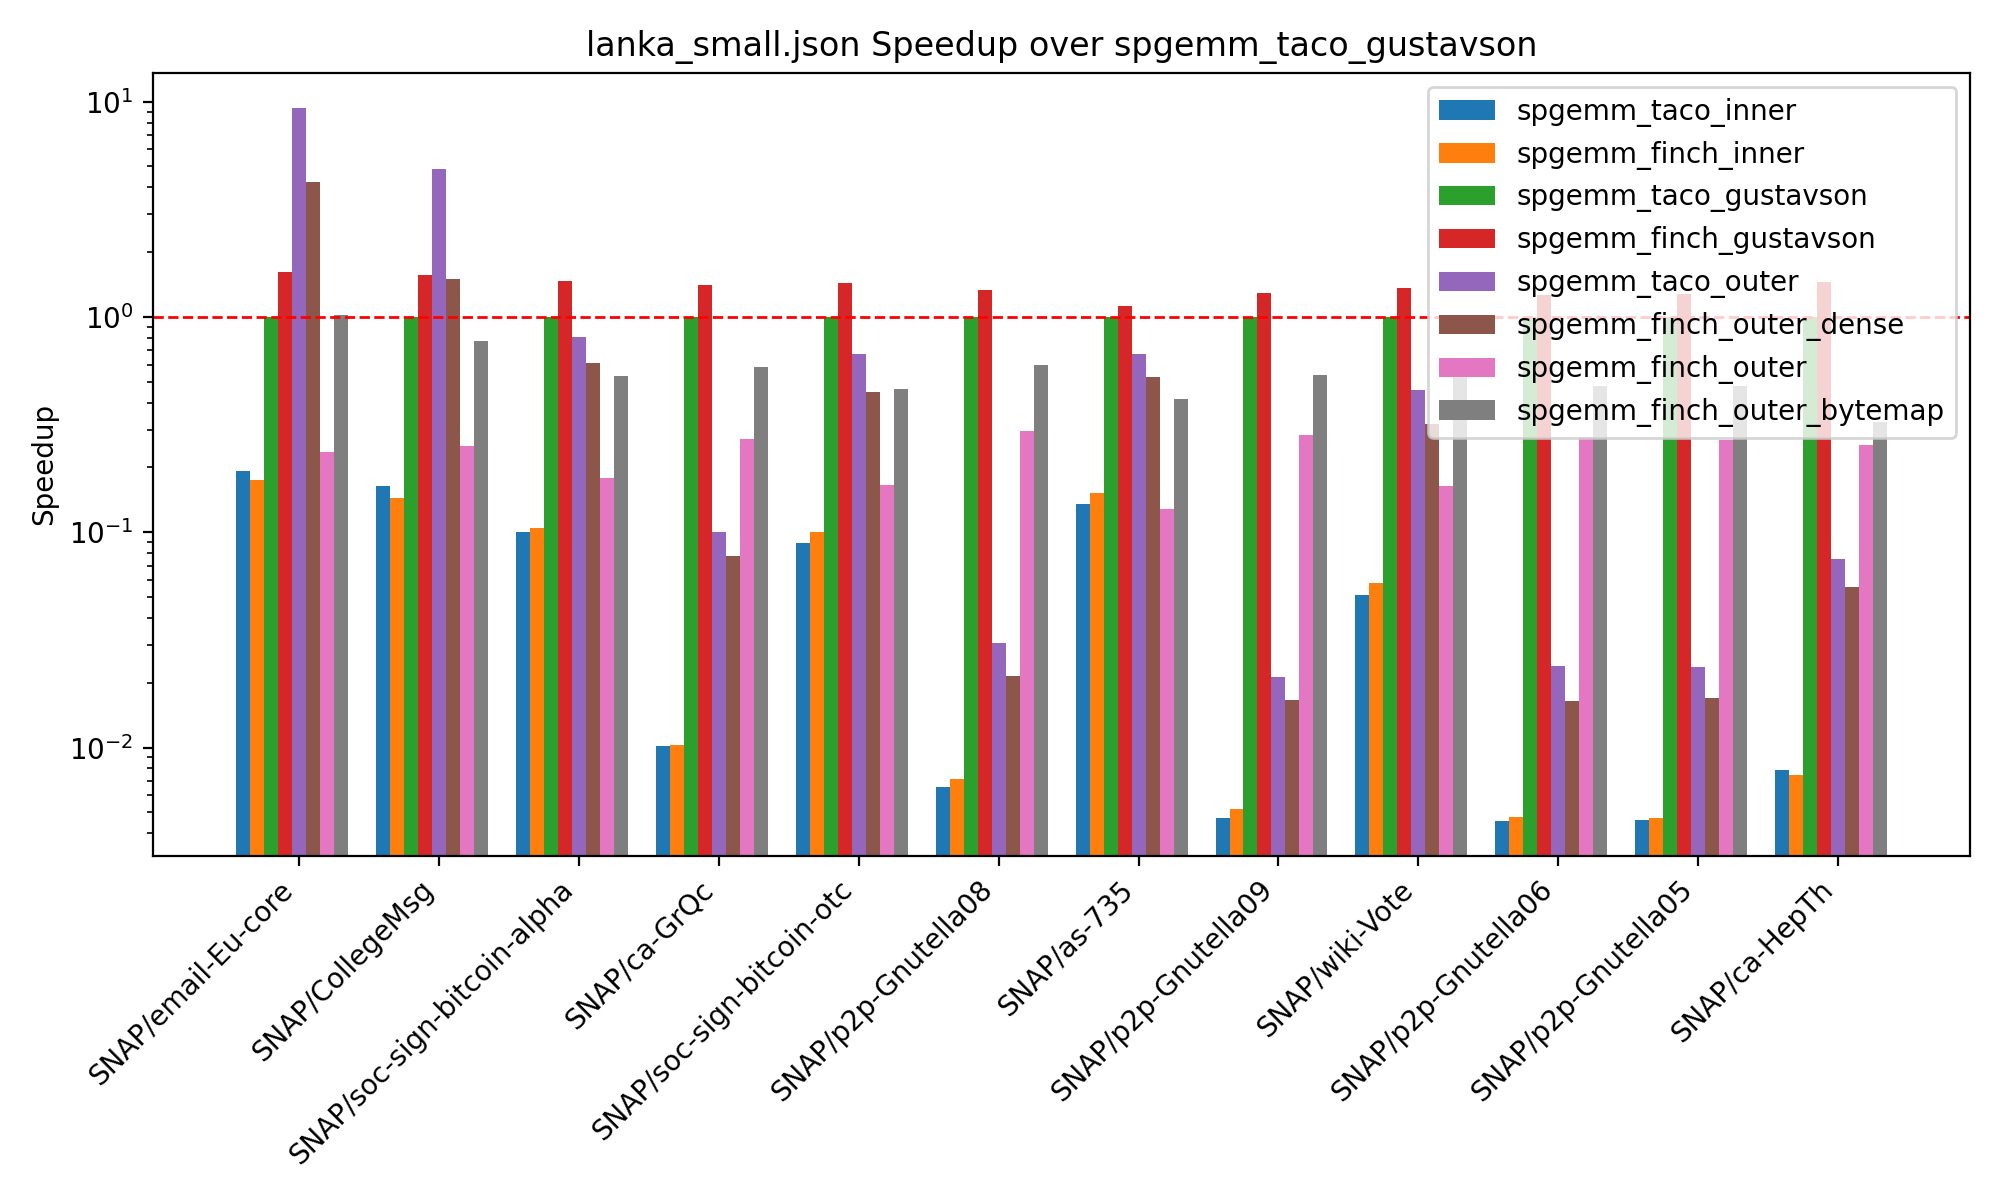
\includegraphics[width=\linewidth]{spgemm_small_speedup_log_scale.png}
    \caption{A comparison of several matrix multiplication algorithms between Finch and Taco smaller matrices, ordered from small to big dimension. Note that inner products necessarily requires $O(n^2)$ work and taco's outer products format is dense. Finch can use a sparse outer products format and thus has an asymptotic advantage that becomes evident as the output dimensions grow.}
\end{figure}

\begin{figure}
\label{spgemm_large}
	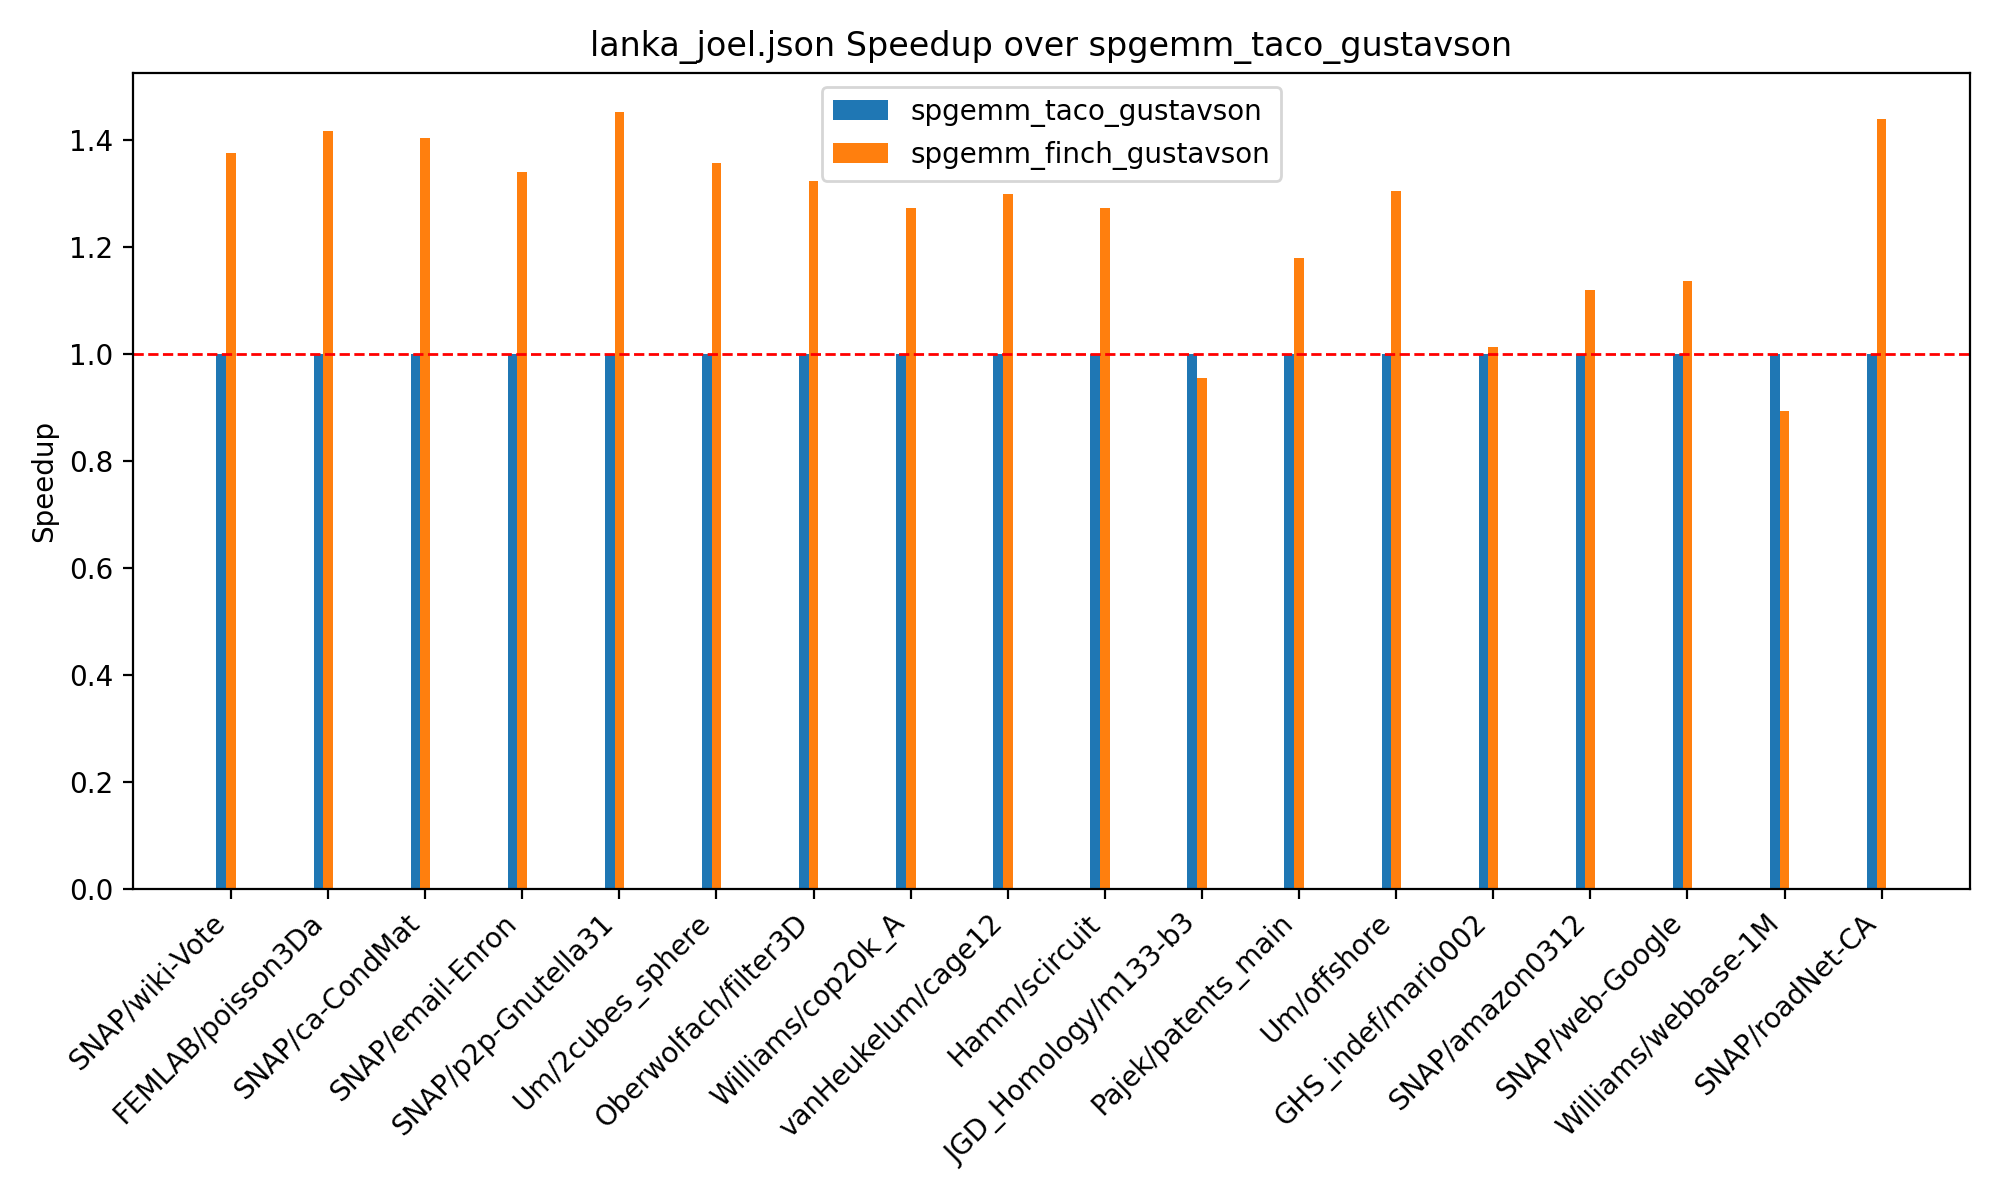
\includegraphics[width=\linewidth]{spgemm_joel_speedup.png}
    \caption{A comparison of gustavson's algorithm between Finch and Taco on some larger matrices}
\end{figure}

Examples that demonstrate performance engineering in a datastructure-driven model

\subsubsection{SpMV}
The sparse matrix-vector multiplication kernel (SpMV) is a common operation in sparse linear algebra with many applications including conjugate gradients, graph algorithms, numerical analysis, and neural networks [cite]. SpMV is a bandwidth bound kernel, and thus historically has been subject to many modifications to improve throughput and reduce the associated control flow [cite]. The wide range of applications unsurprisingly results in a wide range of types of datasets making it an effective kernel to demonstrate the utility of having flexible data formats. 

In this case study, we highlight a few different Finch formats as specified in Table \ref{spmv_tensor_formats}, and the performance effects of conforming a dataset’s structure with its storage format, which Finch's datastructure-driven model enables us to do. Finch also provides the control flow necessary to manipulate data reads and writes, enabling exploitation of multiple structural patterns concurrently (e.g. sparsity \textit{and} symmetry). 


We display speedup relative to TACO, SuiteSparseGraphBLAS, and Julia’s standard library, as depicted in Figures \ref{spmv_sorted} and \ref{spmv_grouped}.  We test using sparse matrices from a large selection of datasets spanning several previous papers: the datasets used by Vuduc et al. to test the OSKI interface \cite{vuduc2005oski}, Ahrens et al. to test a variable block row format partitioning strategy \cite{ahrens_optimal_2021}, and Kjolstad et al. to test the TACO library \cite{kjolstad_tensor_2017}. Additionally, we included the SNAP graph collection to test with boolean matrices. We also created several synthetic matrices containing bands or blocks of varying sizes as well as a permutation matrix to encapsulate a few additional use cases. The dense vector is randomly generated. We tested using the row-major and column-major Finch programs in Figure \ref{spmv_programs} as well as the symmetric program where applicable; the performance displayed for Finch on each dataset in Figure \ref{spmv_grouped} is the fastest among the formats and programs we tested. Column-major SpMV consistently performs better than row-major SpMV (an average of 1.36x better) in TACO so we use column-major SpMV in TACO as our baseline.

% TODO: make this be 3 columns
\begin{figure}
    \begin{minipage}[t]{0.315\textwidth}
        \vspace{0pt} % Add this to ensure top alignment within minipage
        \begin{minted}{julia}
            @finch begin
                y .= 0
                for j = _, i = _
                    y[i] += A[i, j] * x[j]
                end
                return y
            end
        \end{minted}
    \end{minipage}%
    \begin{minipage}[t]{0.315\textwidth}
        \vspace{0pt} % Add this to ensure top alignment within minipage
        \begin{minted}{julia}
            @finch begin
                y .= 0
                for j = _, i = _
                    y[j] += A[i, j] * x[i]
                end
                return y
            end
        \end{minted}
    \end{minipage}
    \begin{minipage}[t]{0.36\textwidth}
        \vspace{0pt} % Add this to ensure top alignment within minipage
        \begin{minted}{julia}
            @finch begin
                y .= 0
                for j = _
                    let x_j = x[j]
                        y_j .= 0
                        for i = _
                            let A_ij = A[i, j]
                                y[i] += x_j * A_ij
                                y_j[] += A_ij * x[i]
                            end
                        end
                        y[j] += y_j[] + diag[j] * x_j
                    end
                end
                return y
            end
        \end{minted}
    \end{minipage}
    \caption{Finch SpMV Programs}
    \label{spmv_programs}
\end{figure}



\begin{table}[htbp]
    \centering
    \caption{SpMV Tensor Formats}
    \label{spmv_tensor_formats}
    \begin{tabular}{|l|l|l|l|}
        \hline
        \textbf{Outer Level} & \textbf{Inner Level} & \textbf{Scalar Values} & \textbf{Style of Matrix}\\
        \hline
        \multirow{6}{*}{Dense} & \multirow{2}{*}{SparseList} & Element & sparse, real-valued matrices \\
        \cline{3-4} 
        & & Pattern & sparse, boolean-valued matrices \\
        \cline{2-4} 
        & SparseVBL & Element & real-valued matrices with blocked structure \\
        \cline{2-4}
        & SparseBand & Element & real-valued matrices with diagonal band \\
        \cline{2-4}
        & \multirow{2}{*}{SparsePoint} & Element & real-valued matrices with one value per row \\
        \cline{3-4} 
        & & Pattern & matrix with runs of true or false \\
        \hline 
    \end{tabular}
\end{table}



\subsubsection{Tensor Formats}
We found that the SpMV performance was superior for the level format that best paralleled the structure of the tensor. We consider the Dense(SparseList(Element)) format with the column-major SpMV program to be the Finch baseline as it is the closet analog to the sparse matrix format and SpMV program in other libraries.  

Namely, matrices with a clear blocked structure like exdata\_1, TSOPF\_RS\_b678\_c1, and heart3 performed notably well with the SparseVBL format with speedups of 2.16, 1.55, and 1.30 relative to TACO, while the baseline format had slowdowns of 0.71, 0.53, and 0.92 relative to TACO. Furthermore, the synthetic Toeplitz banded matrices we constructed performed the best with the SparseBand matrix, in particular with the toeplitz\_large\_band and the toeplitz\_medium\_band matrices having a speedup of 1.98 and 1.64 relative to TACO, while the baseline format had slowdowns of 0.84 and 0.51 relative to TACO.

There were also significant advantages of using the Pattern format instead of the Element format to represent scalar values in the matrices when these values were boolean, such as matrices in the SNAP collection which represent graph datasets are boolean. For example, the SparseList-Pattern for email-Eu-core resulted in a speedup of 2.51, while the SparseList-Element format resulted in a slowdown of 1.84 over TACO.

\begin{table}[htbp]
    \centering
    \caption{SpMV Sample Matrices}
    \label{spmv_sample_matrices}
    \begin{tabular}{|m{3cm}|c|c|c|}
        \hline
        \textbf{Spy} & \textbf{Group / Name} & \textbf{Dimensions} & \textbf{Best Finch Format}\\
        \hline
        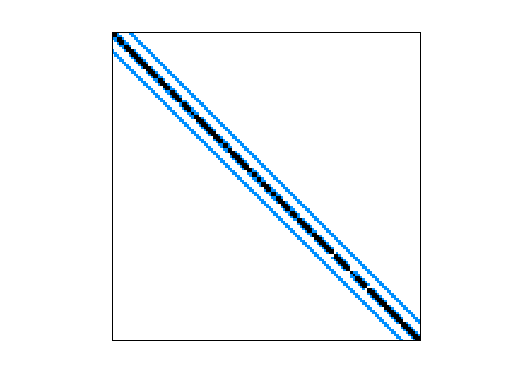
\includegraphics[width=3cm]{spmv_matrices/saylr4.png} & HB/saylr4 & 3,564 x 3,564 (22,316) & Symmetric SparseList \\
        \hline 
        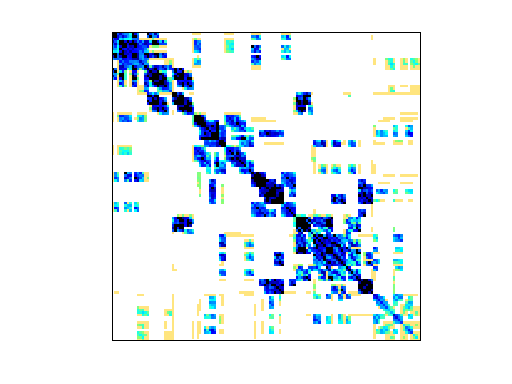
\includegraphics[width=3cm]{spmv_matrices/heart3.png} & Norris/heart3 & 2,339 x 2,339 (680,341) & SparseVBL \\
        \hline 
        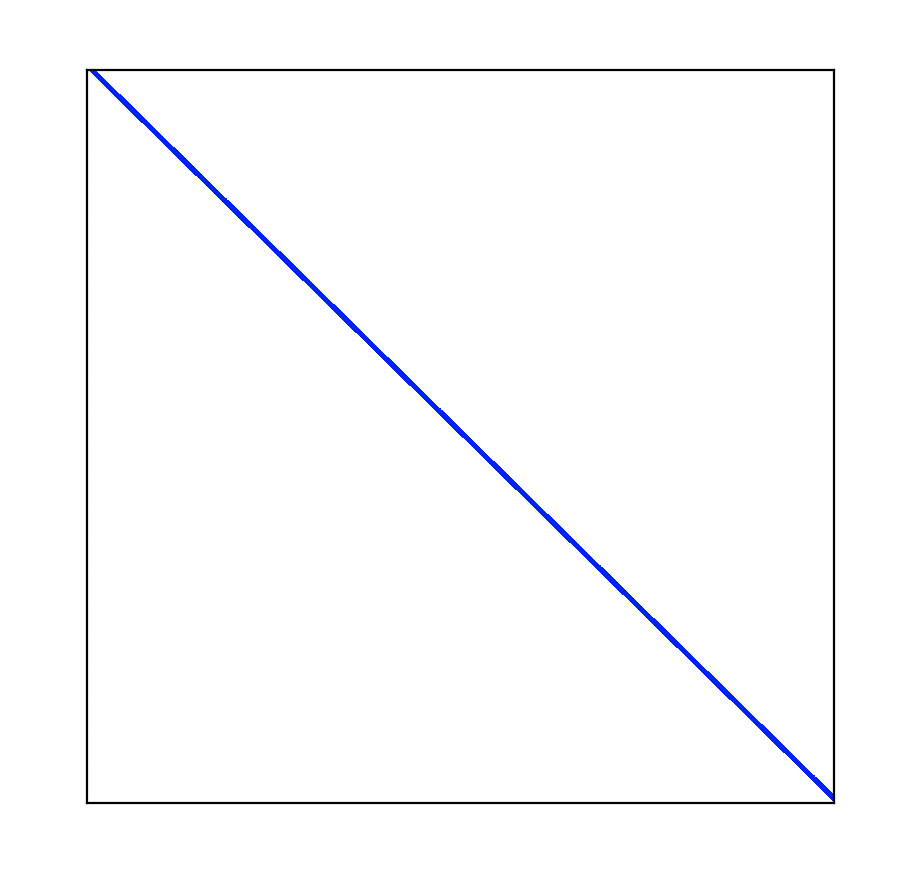
\includegraphics[width=3cm]{spmv_matrices/toeplitz_large_band.png} & toeplitz\_large\_band  & 10,000 x 10,000 (1,999,900) & SparseBand \\
        \hline
        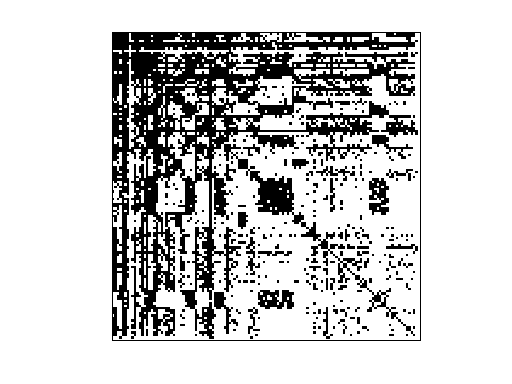
\includegraphics[width=3cm]{spmv_matrices/as-735.png} & SNAP/as-735 & 7,716 x 7,716 (26,467) & Symmetric SparseList-Pattern \\
        \hline
    \end{tabular}
\end{table}


\begin{table}[htbp]
    \centering
    \caption{SpMV Sample Matrices}
    \label{spmv_sample_matrices}
    \begin{tabular}{|l|c|c|c|c|}
     \textbf{Spy} &
     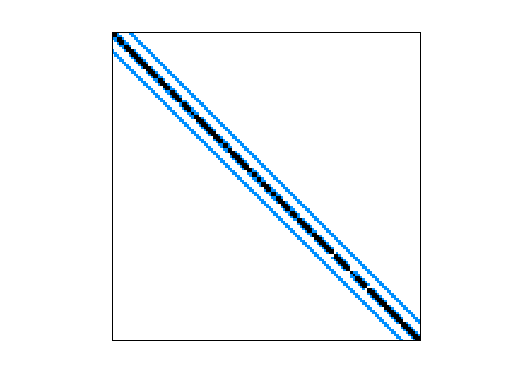
\includegraphics[width=3cm]{spmv_matrices/saylr4.png} &
     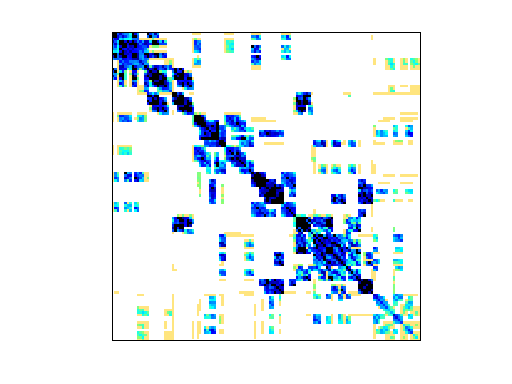
\includegraphics[width=3cm]{spmv_matrices/heart3.png} &
     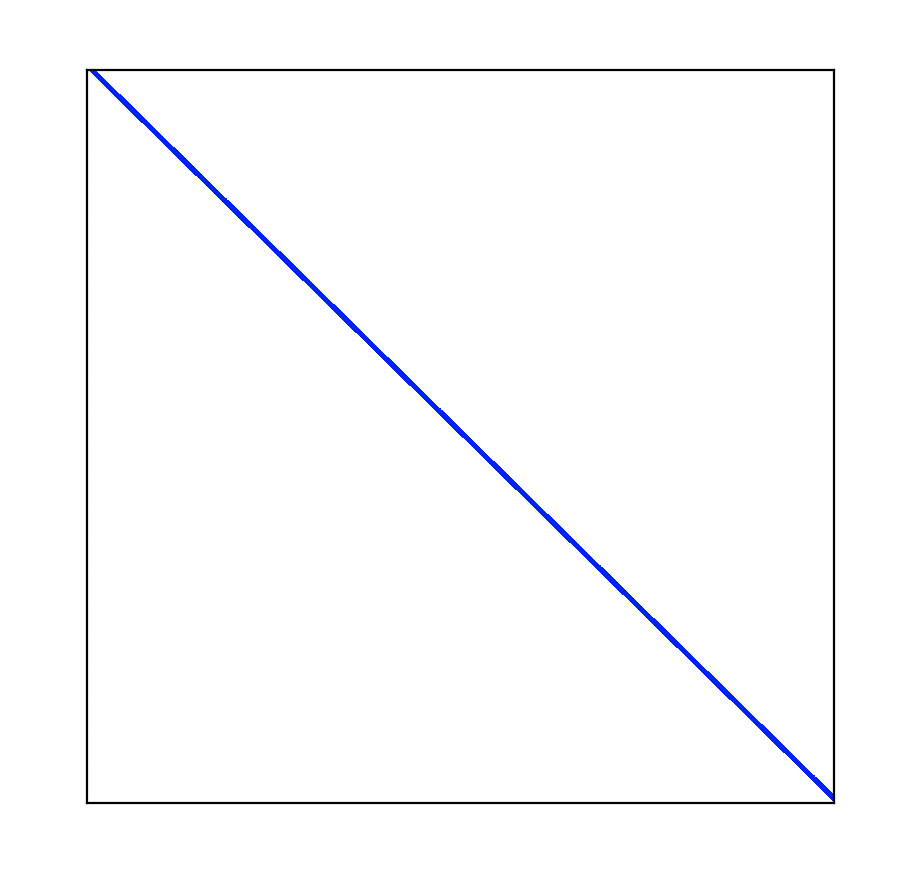
\includegraphics[width=3cm]{spmv_matrices/toeplitz_large_band.png} & 
     
    \end{tabular}
\end{table}



\subsubsection{Symmetric SpMV}
Finch enables us to exploit symmetry in the sparse matrix of the SpMV kernel by providing the capabilities to reuse memory reads and insert control flow logic to restrict iterations to either the lower or upper triangle of the sparse matrix. We can apply this strategy with any level format. Every symmetric matrix in the SparseList and SparseList-Pattern formats has better performance when we use a Finch SpMV program that takes advantage of this symmetry. However, the regular row- or column-major Finch SpMV programs have better performance for symmetric matrices than the symmetric Finch SpMV program for the other more specialized formats, likely because we need in-order accesses to fully capitalize on the specialized storage. Symmetric SpMV with the SparseList level format in Finch results in an average of 1.27x speedup over TACO and symmetric SpMV with the SparseList-Pattern format in Finch results in an average speedup of 1.21x over TACO. Notably, there is a 1.91x speedup for the HB/saylr4 matrix over TACO. 

% Perhaps add the following section again in a future iteration of paper
% \subsubsection{4D Blocked SpMV}
% Finch also provides us the capability of writing an SpMV kernel [point to figure] that computes the output in blocks. Specifically, we rewrite an n x n matrix as a n/b x n/b x b x b 4-dimensional tensor and the vector as an n x n/b matrix where b is the block-size. We represent the blocked matrix with a SparseList as its second level (i.e. of format Dense(SparseList(Dense(Dense(Element(0.0)))))) so that only the non-zero blocks are stored. Then, we perform SpMV on each b x b block individually. Note that although SparseVBL already stores consecutive nonzeros in blocks, the benefit of a 4D-blocked kernel is that it additionally computes the output block by block. This method enables us to take advantage of spatial and temporal locality via register reuse [cite].

% We evaluated the 4D-blocked kernel on the Kronecker product of a neural network matrix (erdos-renyi, with sparsity p = ?) with a blocked matrix of size 10x10 and a dense and randomly generated vector. We found a 1.04x speedup to TACO, indicating comparable performance, and a 1.35x speedup to computing a non-blocked SpMV with the SparseVBL format, the fastest performing 2D Finch format for this matrix. 

% Structured matrices with induced dense blocks of equivalent size commonly arise in machine learning applications. In feature extraction, the Kronecker product of image data and a smaller matrix is computed to extract relevant features [cite]. Graph adjacency matrices or Laplacian matrices may also exhibit dense blocks when certain subsets of nodes or edges are densely interconnected. For instance, the adjacency matrix of the Erdös-Renyi random graph has a real symmetric bxb random block at each non-vanishing entry [cite]. 


%Here's a figure with spmv_performance_sorted_(faster_than_taco).png and spmv_performance_sorted_(slower_than_taco).png

\begin{figure}
    \begin{minipage}[t]{0.5\textwidth}
        \vspace{0pt} % Add this to ensure top alignment within minipage
        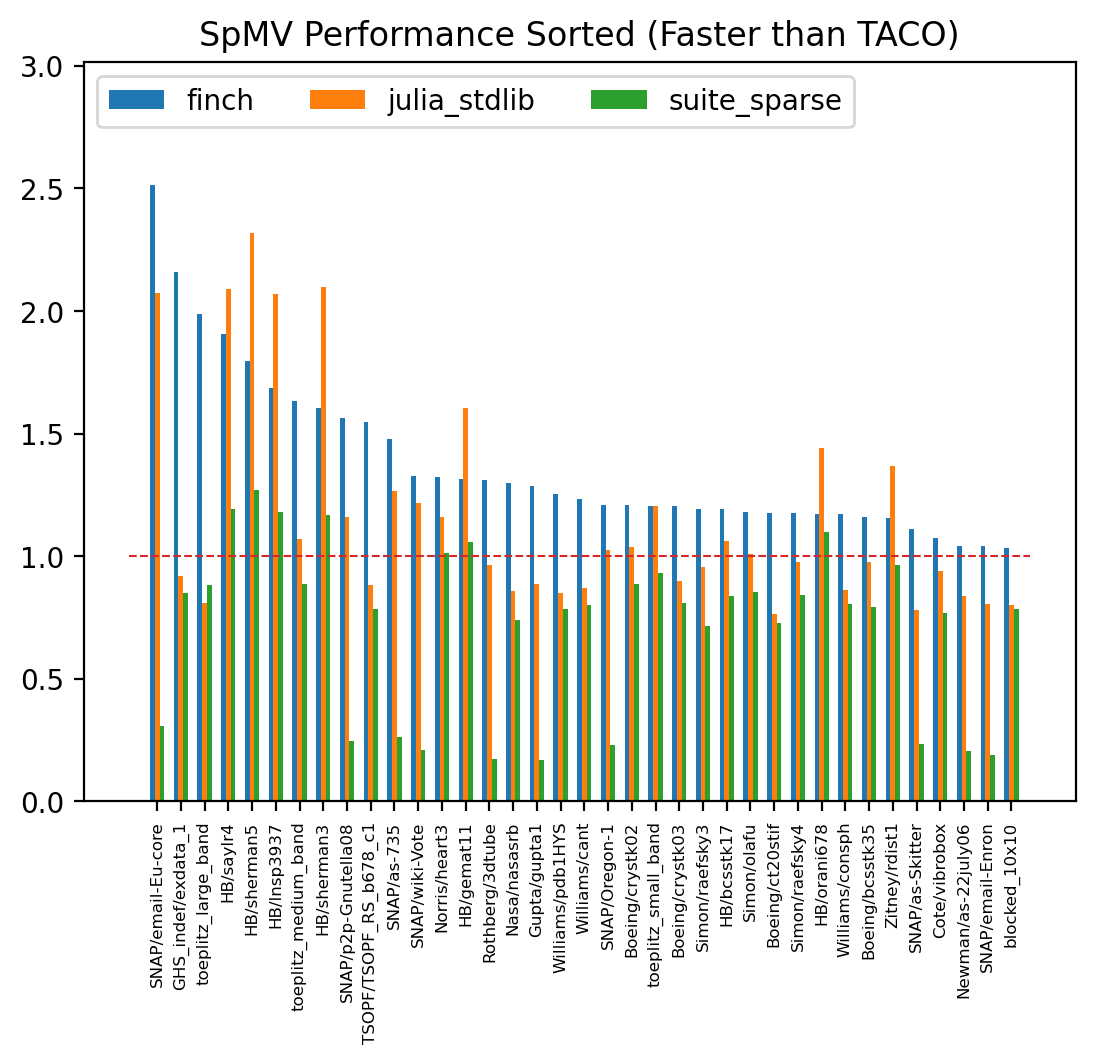
\includegraphics[width=\linewidth]{spmv_performance_sorted_(faster_than_taco).png}
    \end{minipage}%
    \begin{minipage}[t]{0.5\textwidth}
        \vspace{0pt} % Add this to ensure top alignment within minipage
        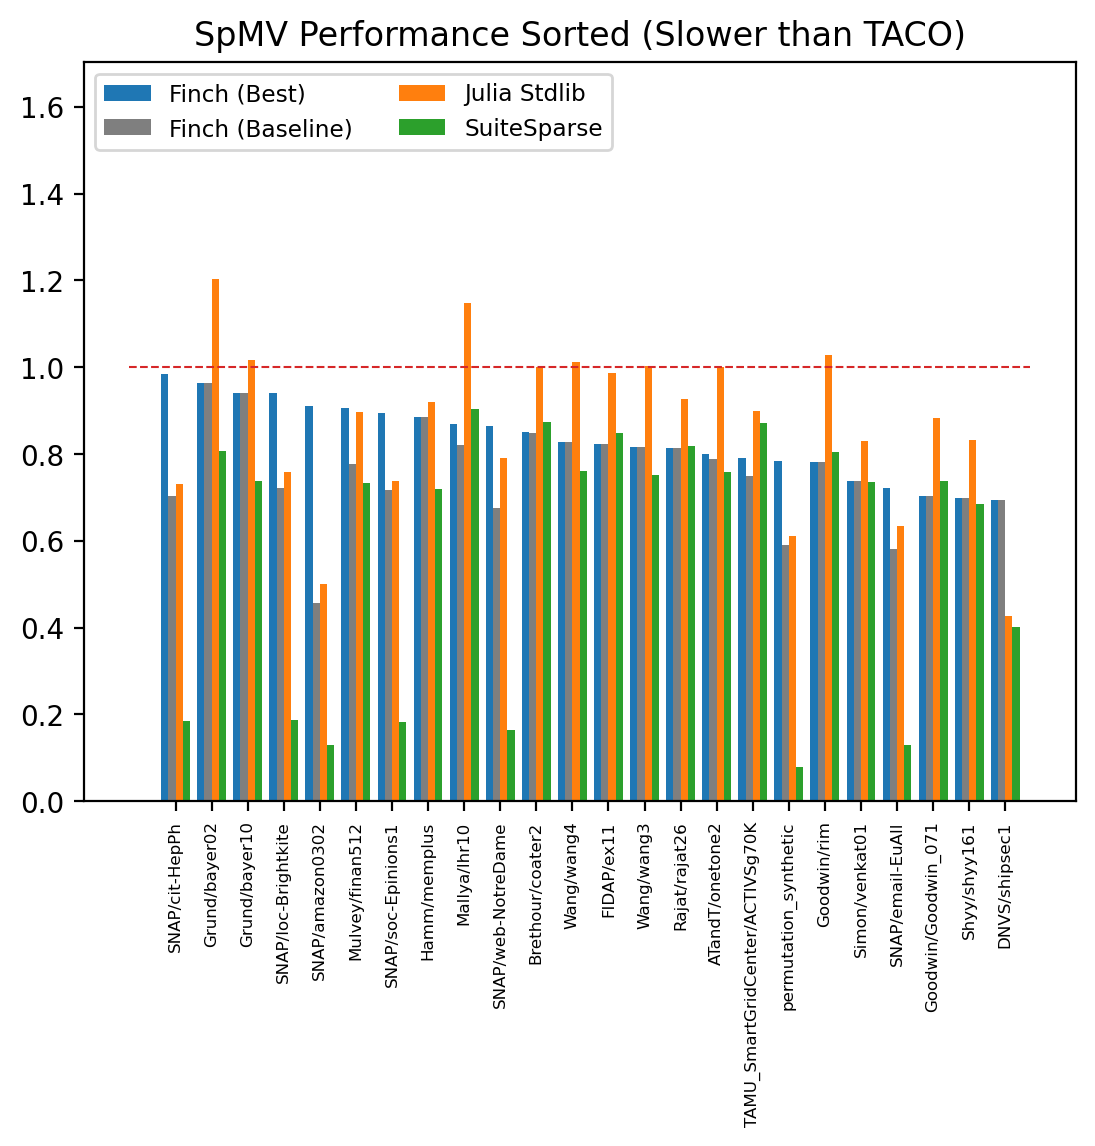
\includegraphics[width=\linewidth]{spmv_performance_sorted_(slower_than_taco).png}
    \end{minipage}
    \caption{Performance of SpMV across various tools.}
    \label{spmv_sorted}
\end{figure}

\begin{figure}
    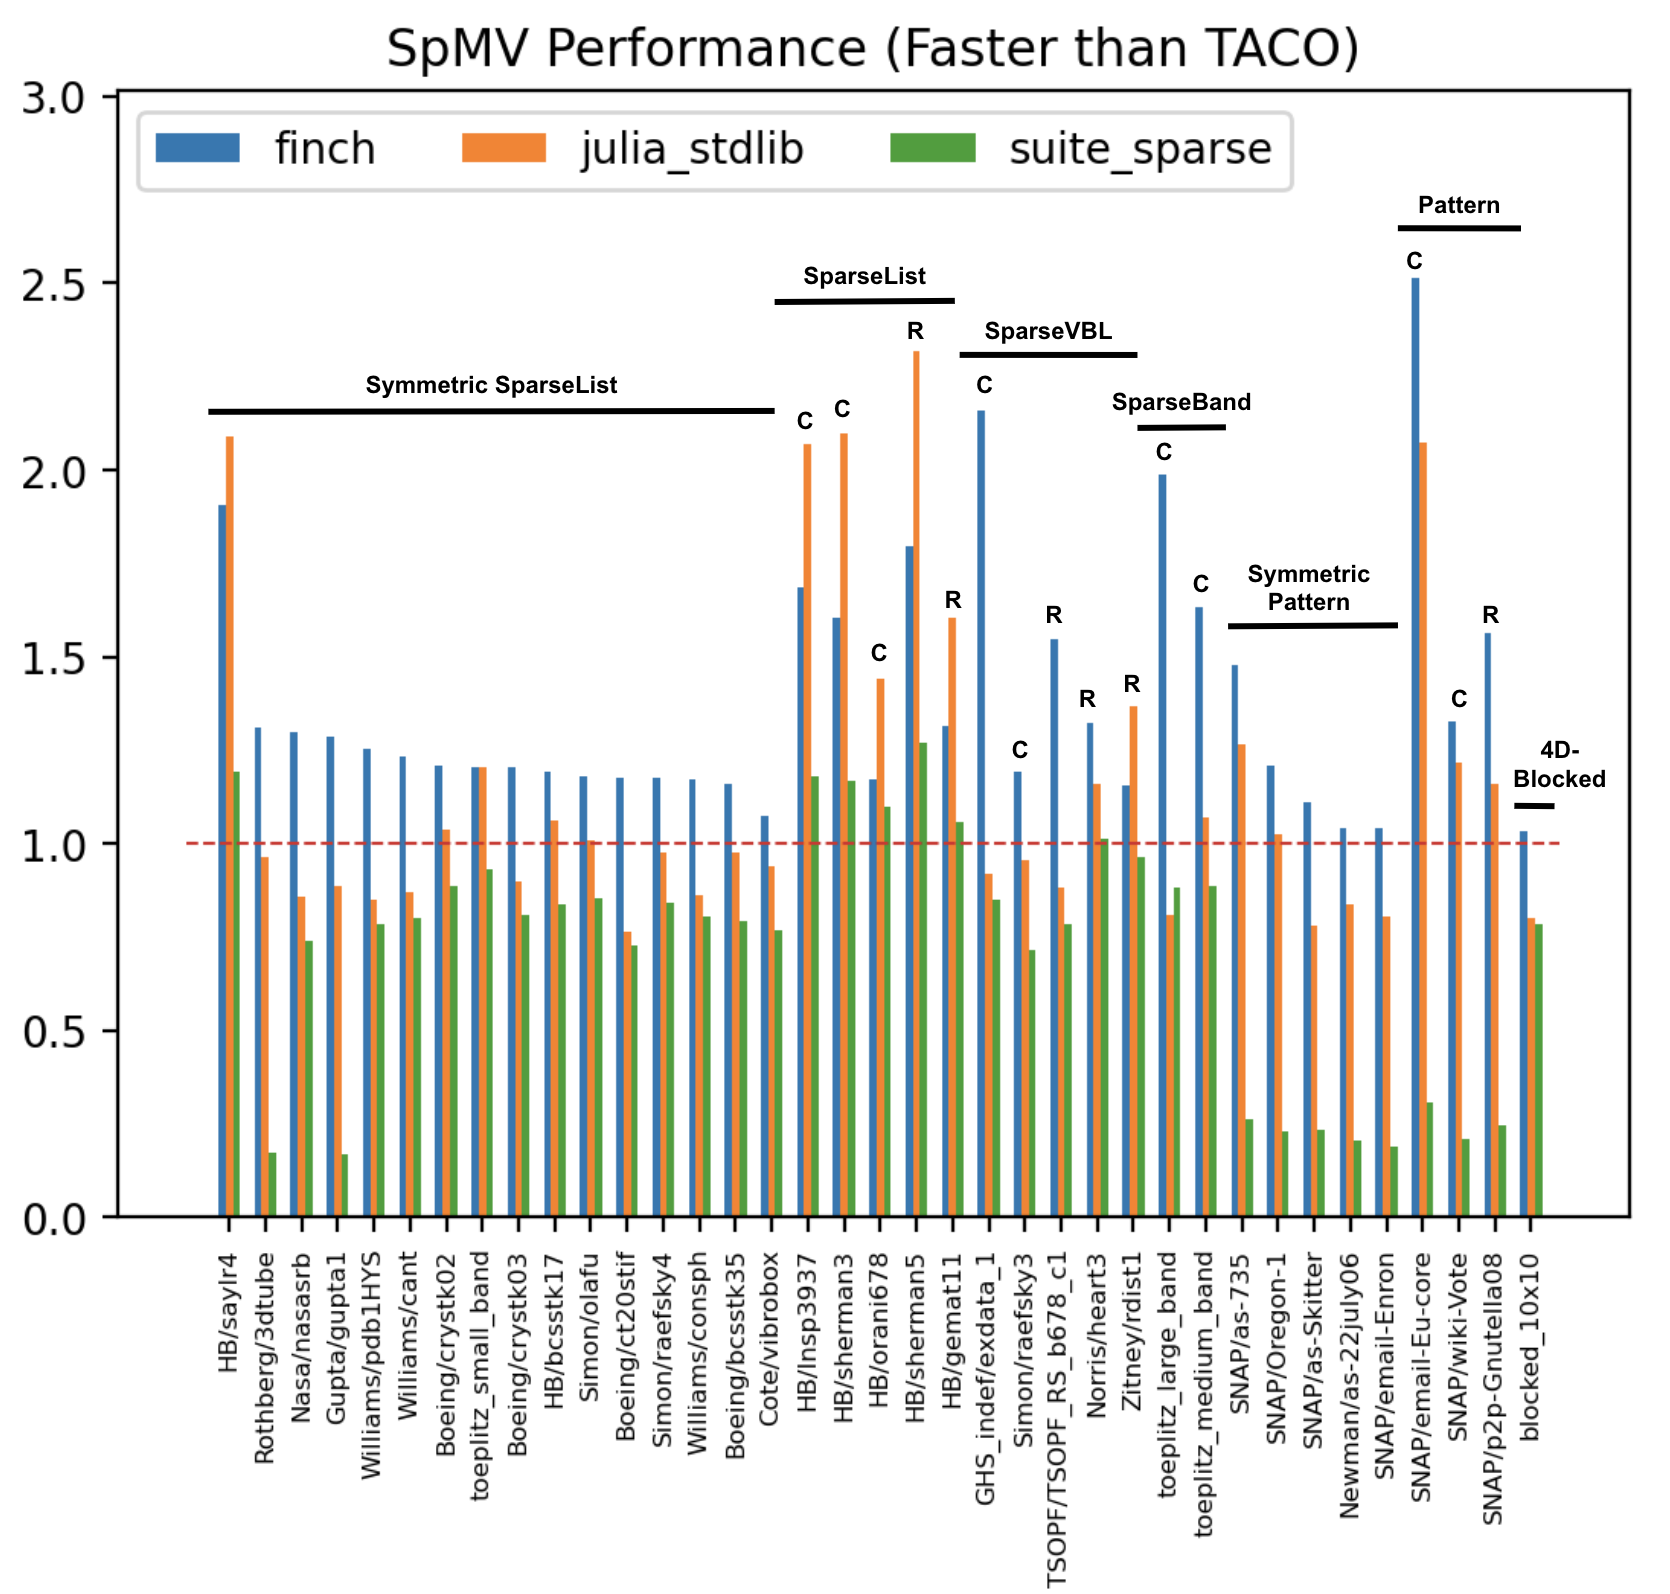
\includegraphics[width=\linewidth]{spmv_performance_grouped.png}
    \caption{Performance of SpMV by Finch format.}
    \label{spmv_grouped}
    \footnotesize The performance displayed for Finch on each dataset is the fastest among the formats we tested. "R" indicates row-major implementation and "C" indicates column-major implementation in Finch. The baseline Finch format is unsymmetric Dense(SparseList(Element)).
\end{figure}

\subsection{Programming over flexible data}

\subsubsection{Image Morphology}

\help{In this section, explain what erosion is, link a few cool images that show erosion, and then explain what the finch kernel looks like. in particular, be sure to point out that we're doing unrolled convolution, and how that maps to the generated code (merging shifted sparse iterators).}

\help{Explain the role of formats in this kernel, how sparseRLE(PAttern) is really the right thing to use here}

\help{Explain that finch can support a bitwise version, and that finch can mask the bitwise kernel too to get performance with a small change to the code}

\help{Point out that masks with SparseRLE can sometimes perform better because they lift the masking out of the inner loop. Talk about hist and also the fact that Finch supports scatter, here and in spgemm.}

\begin{figure}
	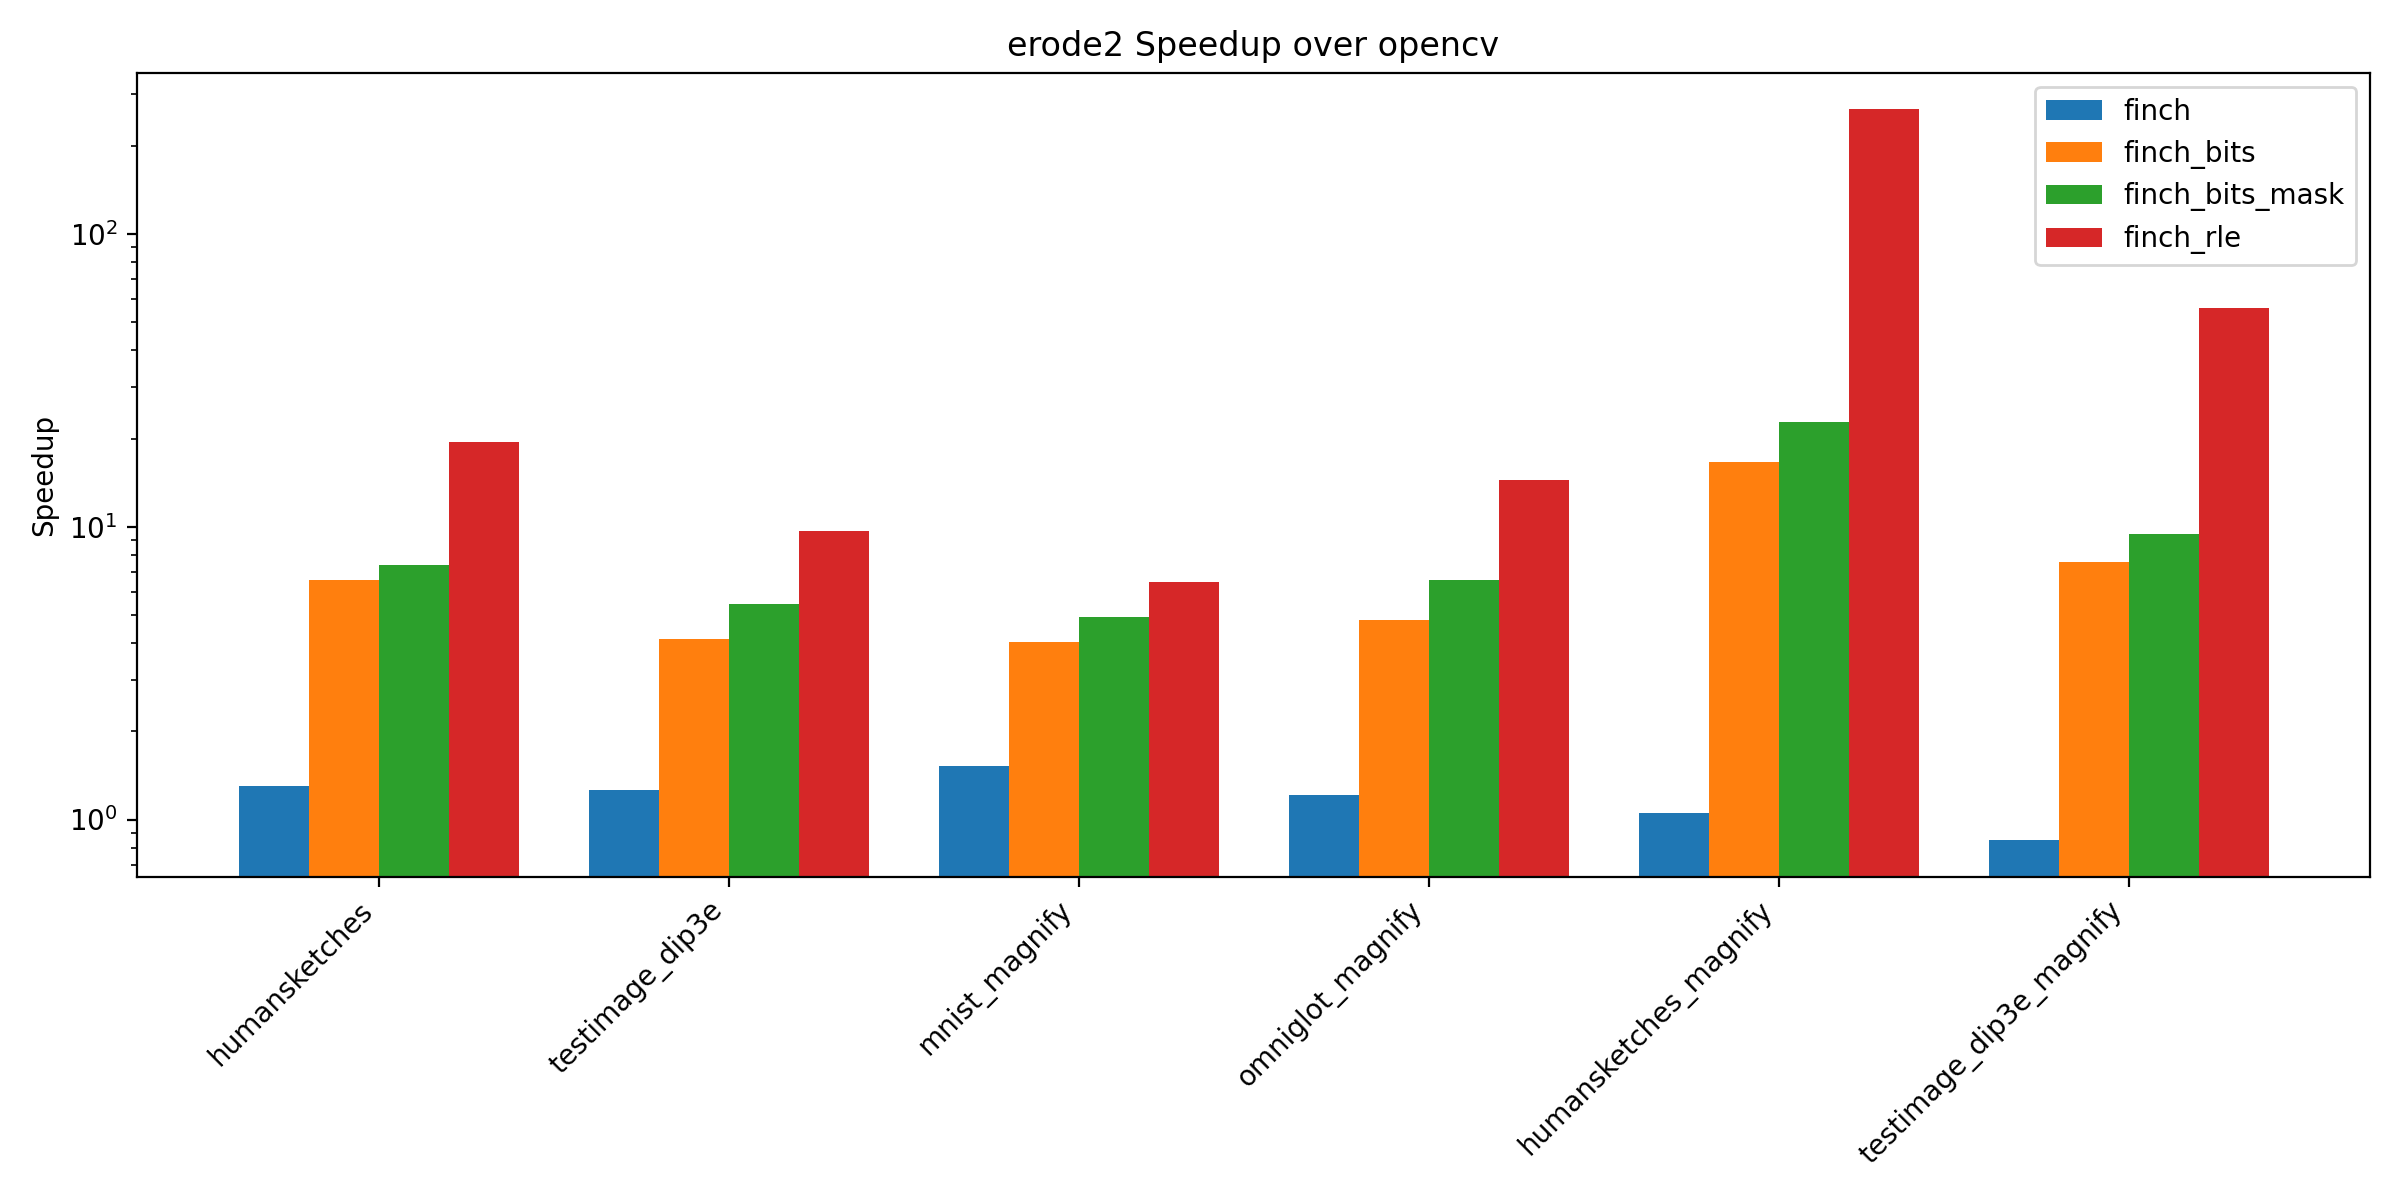
\includegraphics[width=\linewidth]{erode2_speedup_over_opencv.png}
    \caption{Performance of Finch on erosion task (2 iterations).}
\end{figure}

\begin{figure}
	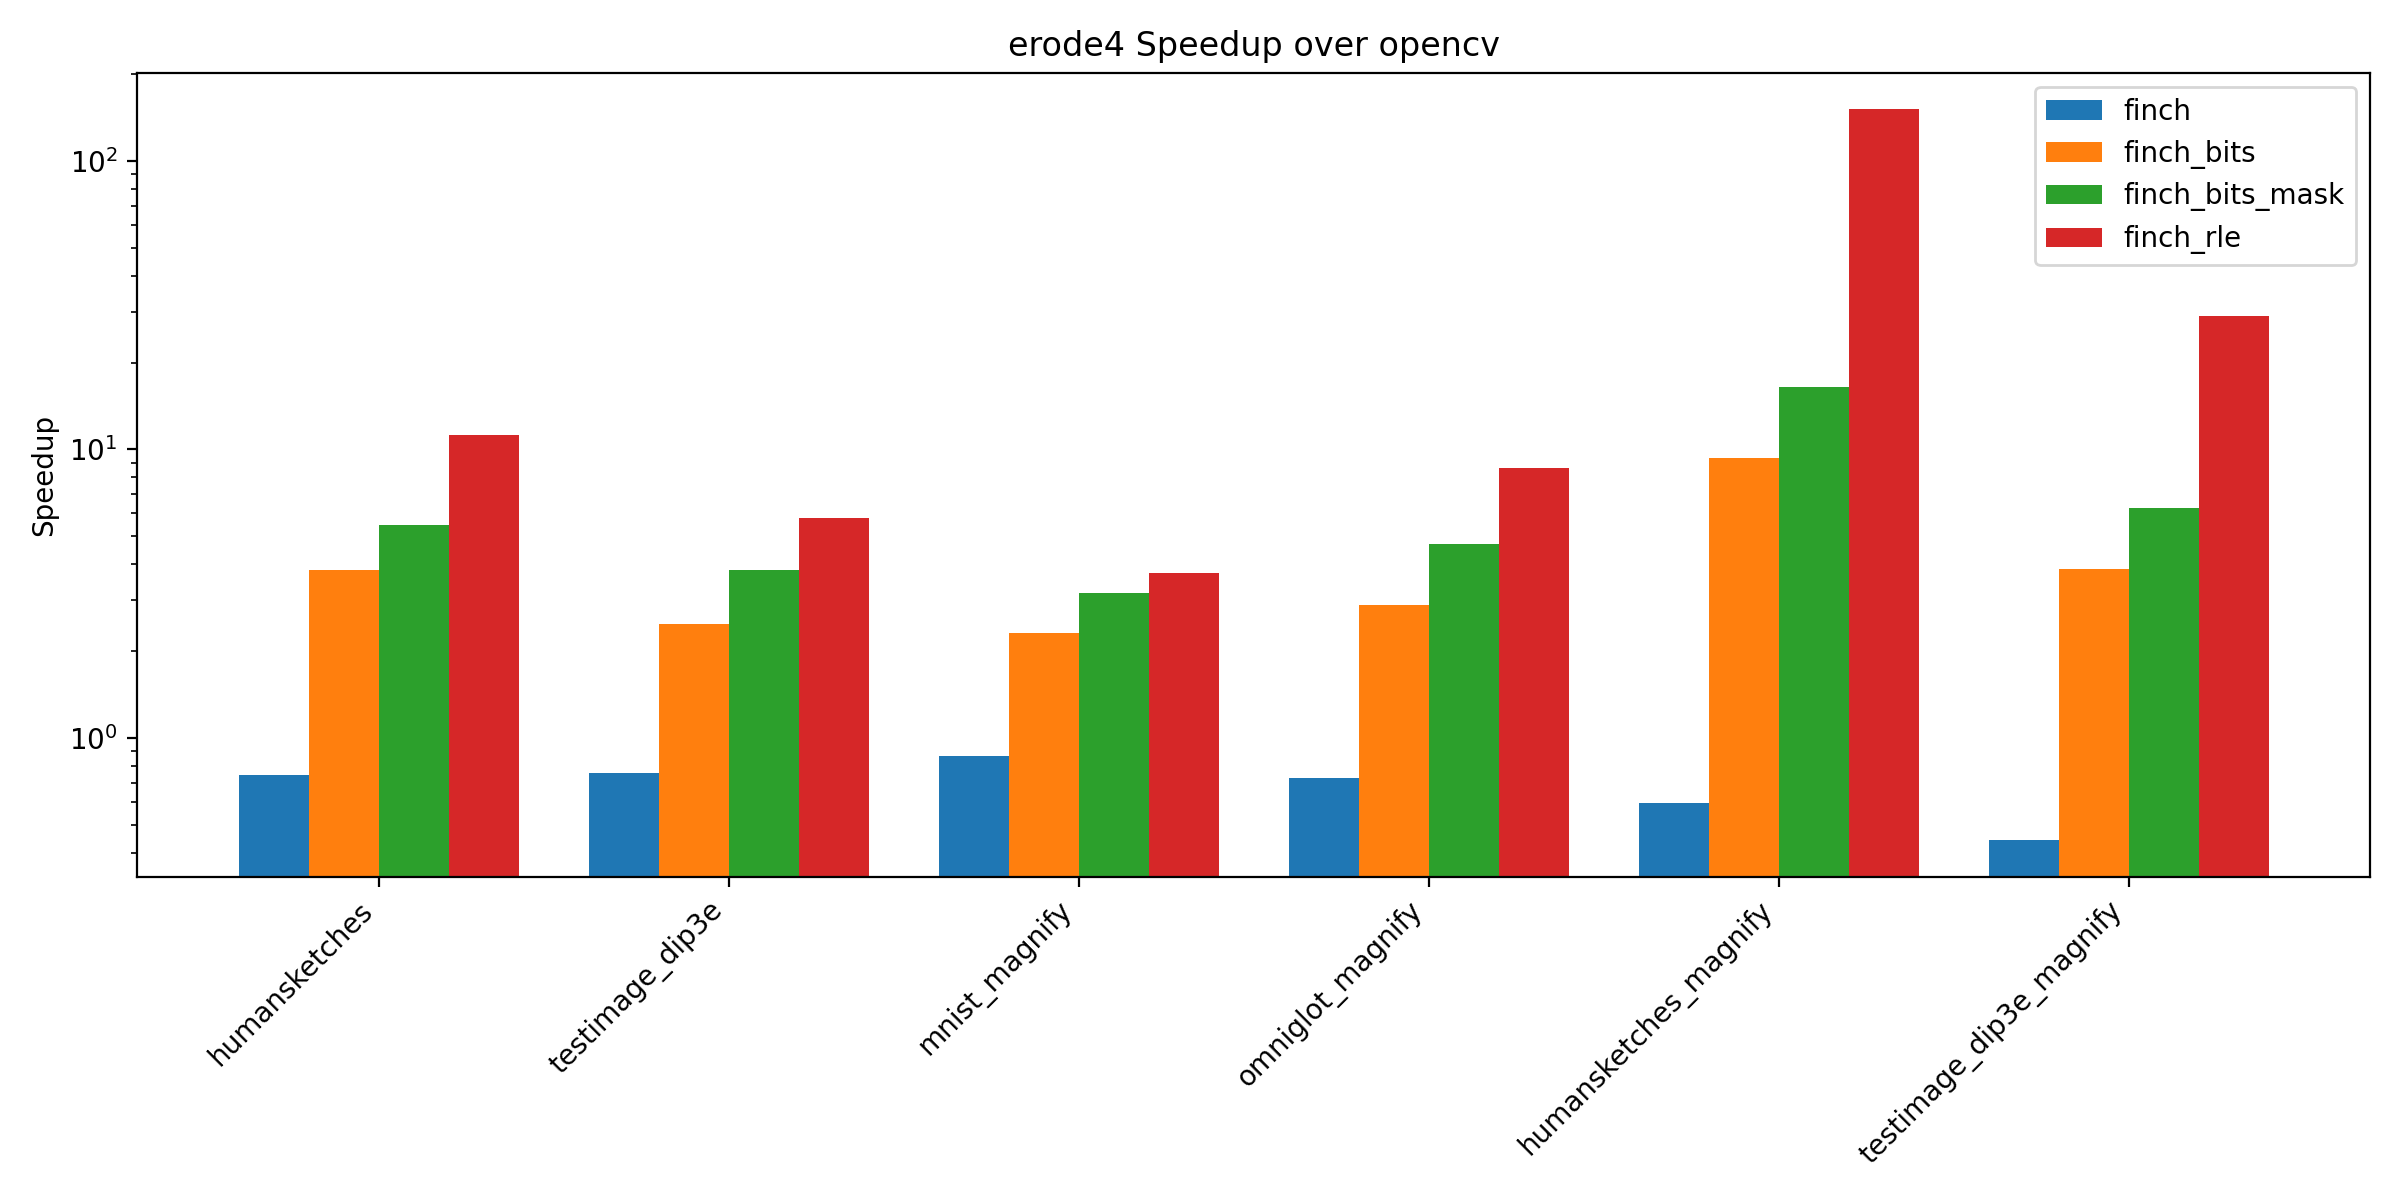
\includegraphics[width=\linewidth]{erode4_speedup_over_opencv.png}
    \caption{Performance of Finch on erosion task (4 iterations).}
\end{figure}

\begin{figure}
	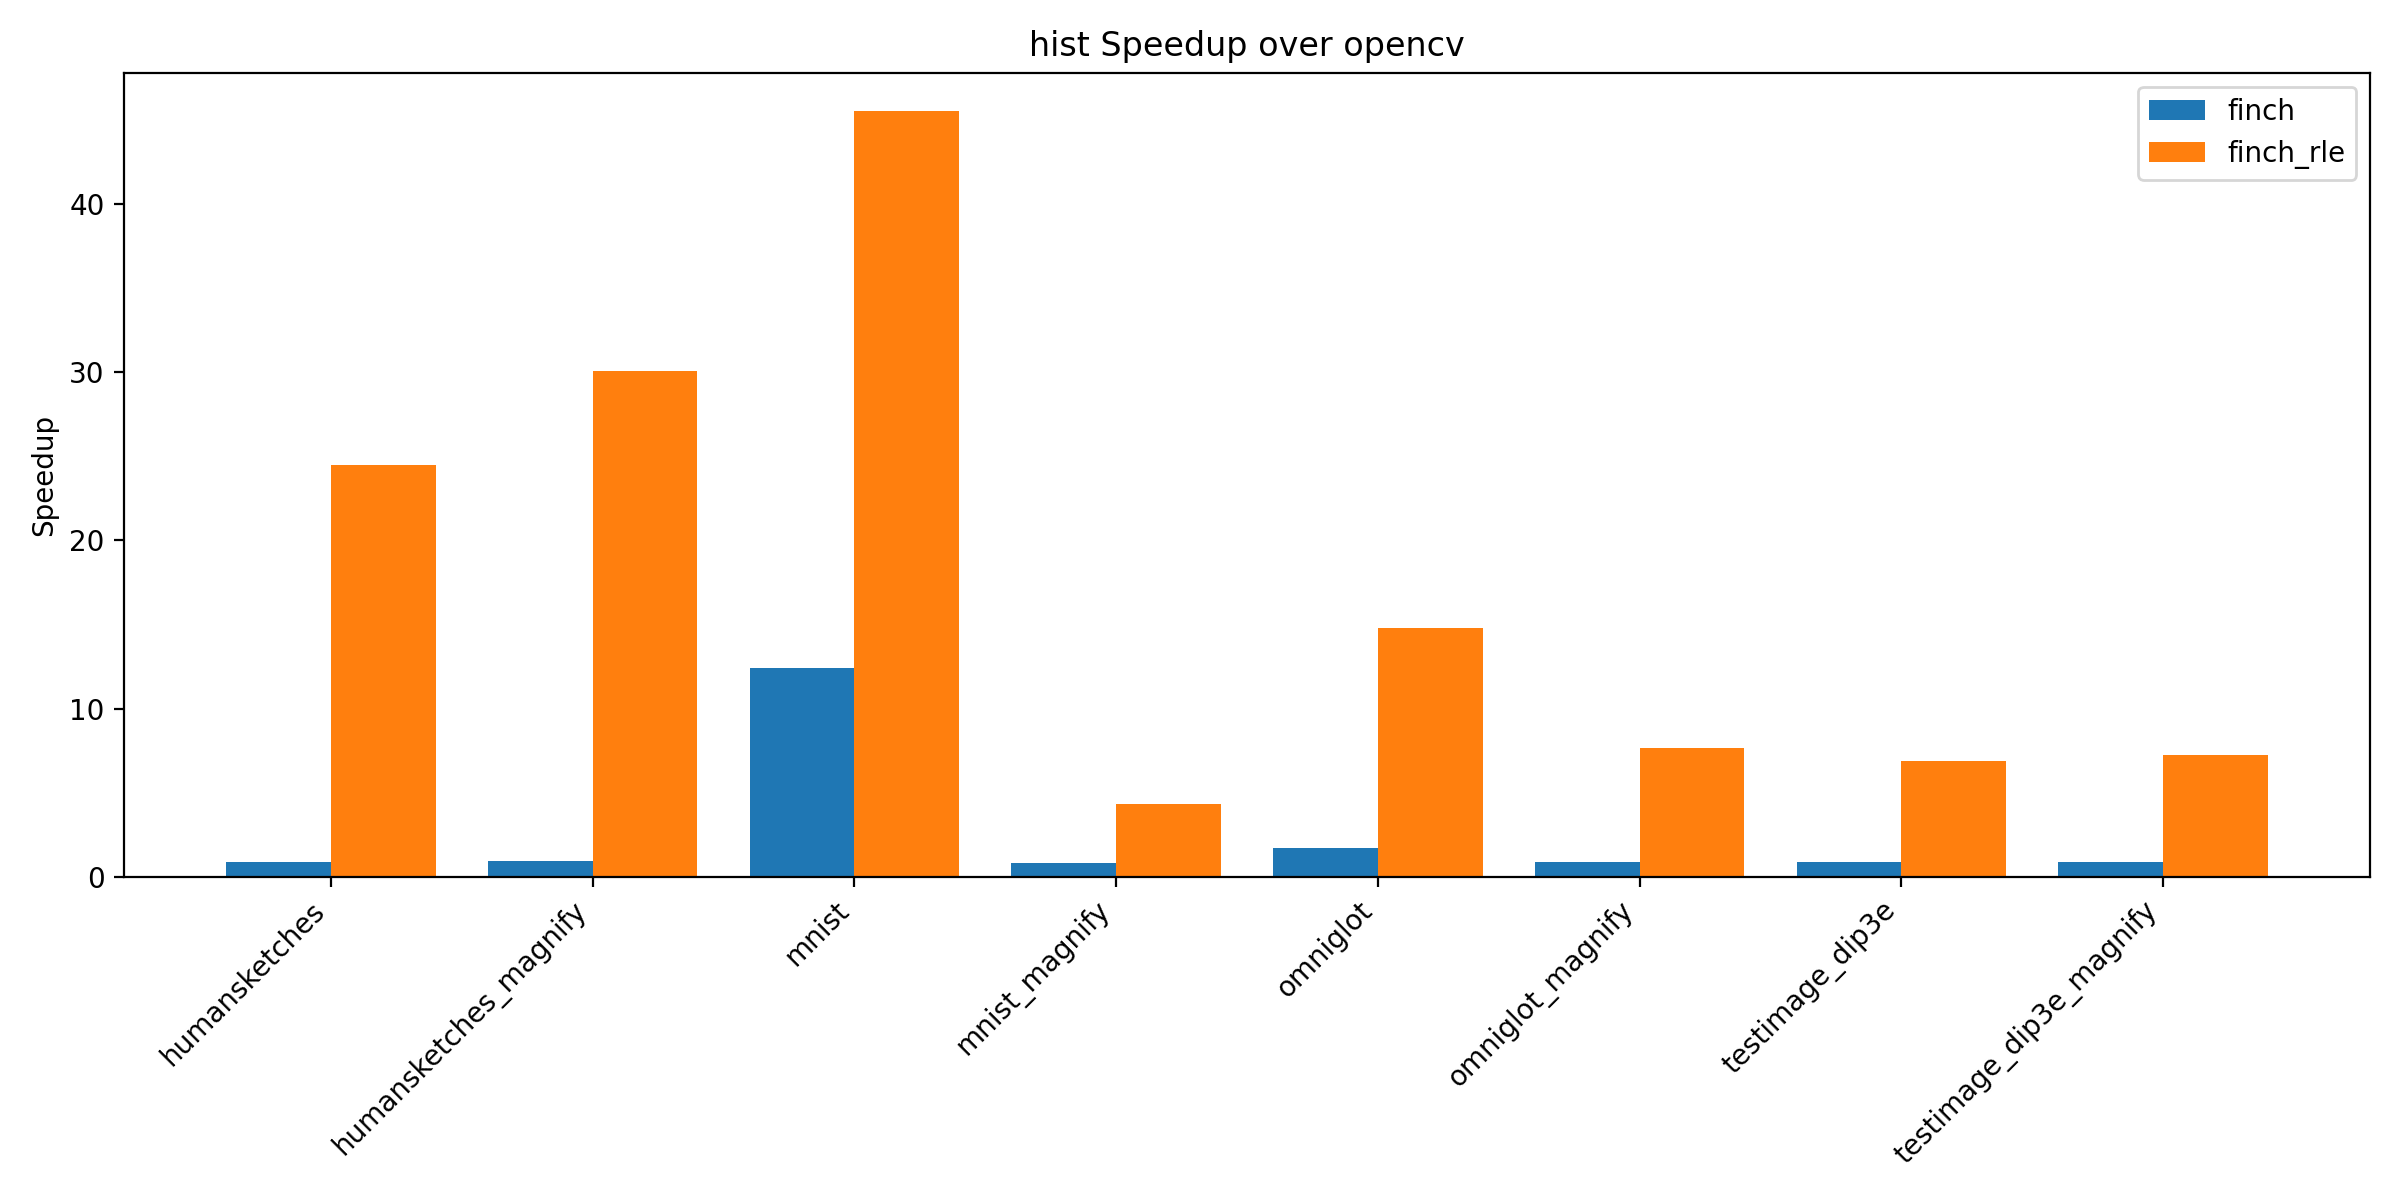
\includegraphics[width=\linewidth]{hist_speedup_over_opencv.png}
    \caption{Performance of Finch on masked histogram task.}
\end{figure}

\subsubsection{Graph Analytics}
\help{In this case, the two main highlights are that Finch can do arbitrary operators (i.e. choose), and that Finch can do early break, and also the different loop orders and multiple outputs. We may need to explain a little bit about what push pull is. For bellman, the main point is that we need multiple outputs, sparse inputs, masks, and sparse outputs with differing formats at differing points.}

To evaluate the capabilities of Finch in graph applications, we its performance for two fundamantal graph applications: Breadth-first search (BFS) and Bellman-Ford single-source shortest path. We used graphs in GraphBLAS~\cite{}, which include road networks (SNAP/roadNet-CA and GAP/GAP-road) where node degrees are bounded and a diametr is very long and scale-free graphs (the others) where the distribution of node degrees follows a power-law distribution and a diameter is very short, direction-optimization~\cite{} is crucial to achiceve high-performance. Direction-optimized BFS uses push and pull traversal to efficiently explore graphs. Push traversal starts from the source node, pushing neighboring nodes into the queue. Pull traversal starts from the target node, exploring predecessors (parents). This approach uses early-break in pull traversal, which is used to terminate the traversal prematurely once the target node is encountered, to avoid unnecessary edge traversal. 

Figure~\cite{graph_result} (a) \changwan{add (a) in fig} shows BFS speedup over Graphs.jl, a BFS implementation with push traversal of Julia. `finch\_push\_only` only uses push traversal, whereas `finch\_push\_pull` applies direction-optimization used in GraphBLAS. Finch supports push/pull traversal, early break, so it supports direction-optimization. Finch additionaly supports the different loop orders and multiple outputs, which also improves the performance. As shown in Figure~\cite{graph_result} (a), direction-optimization significantly improves the performance for scale-free graphs. \changwan{how much average speedup?} GraphBLAS sometimes better than Finch since GraphBLAS incorporates all hardwired optimizations. We believe we will achieve a better performance if we incorporate those optimizations. 



\begin{figure}
	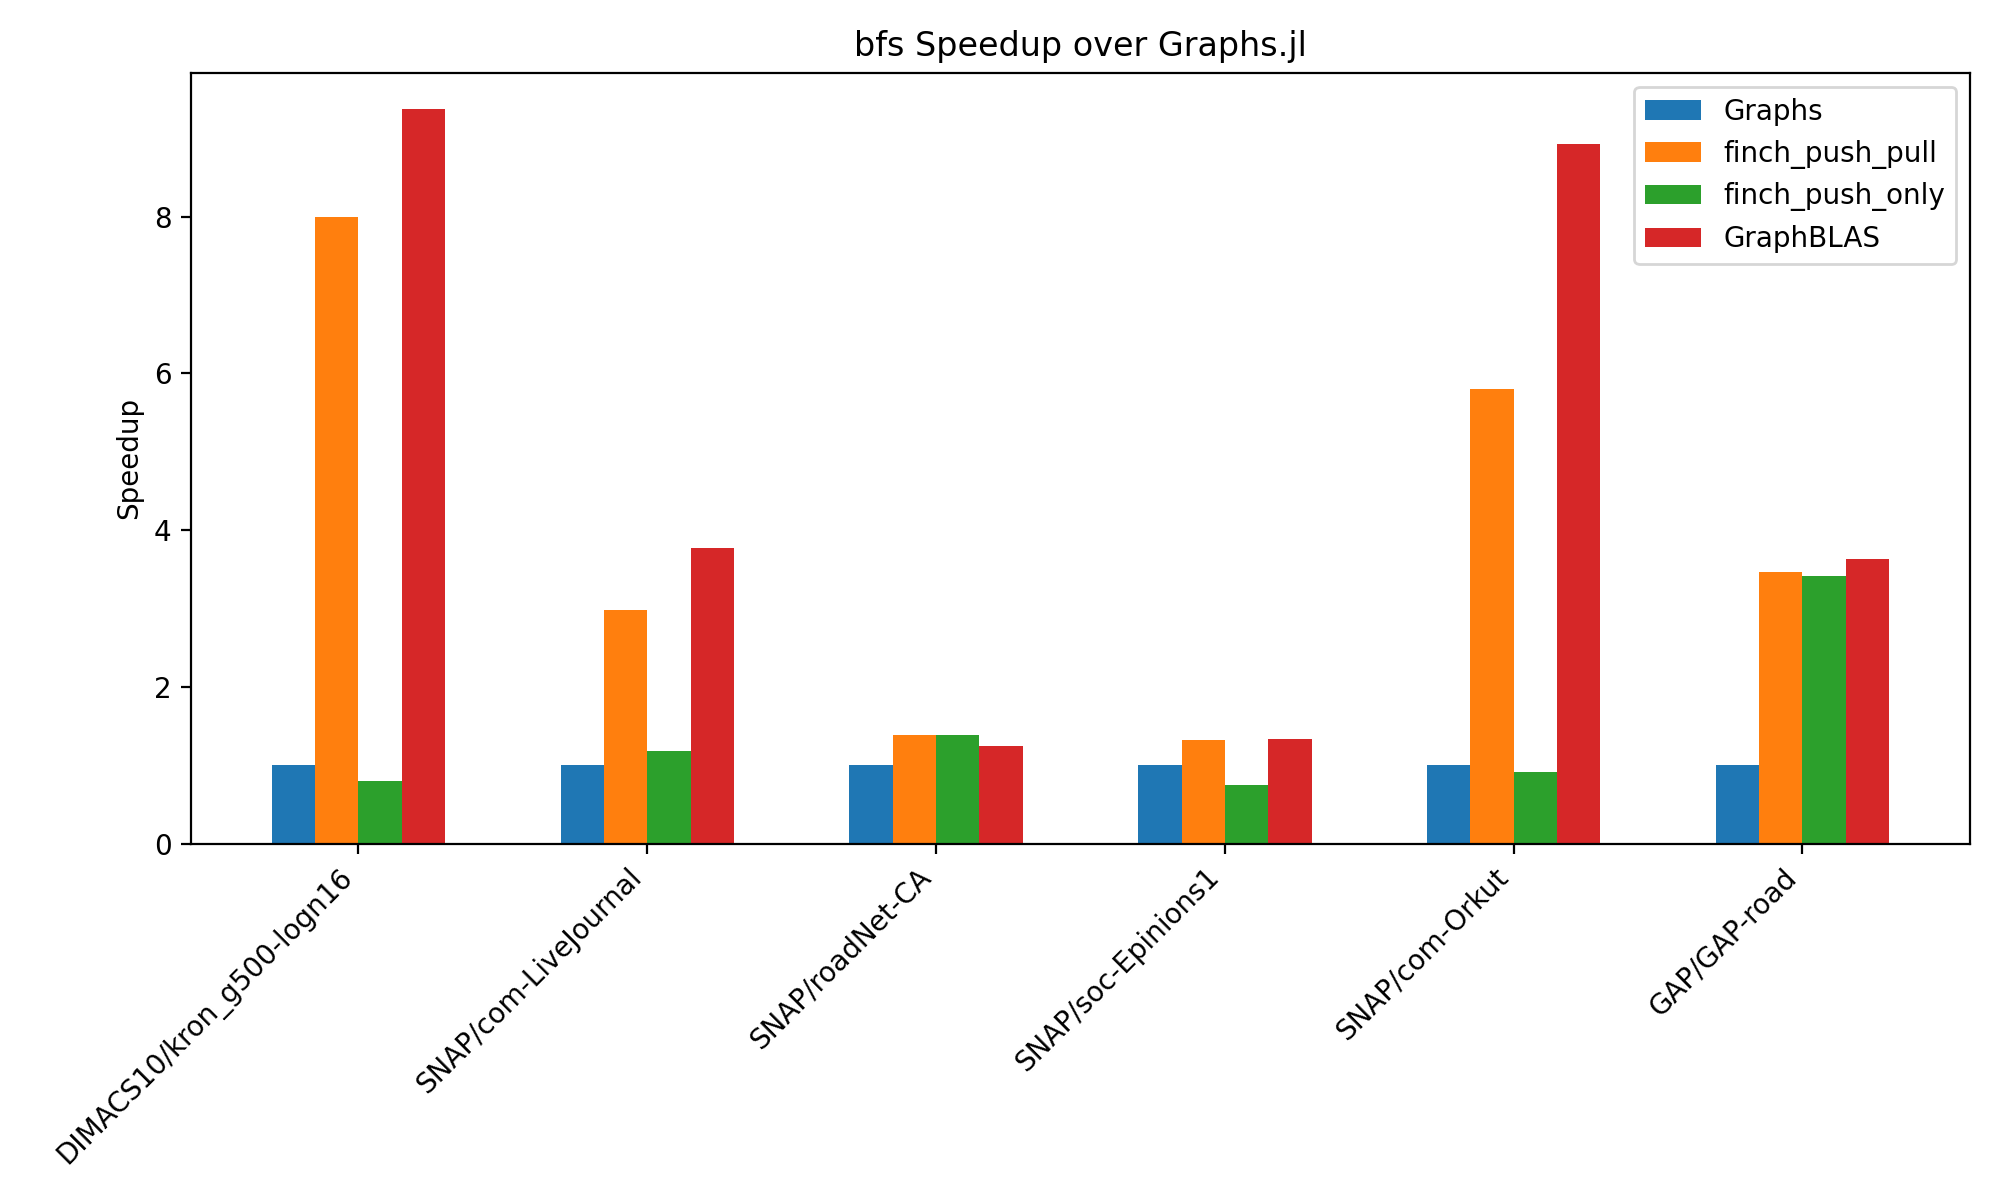
\includegraphics[width=\linewidth]{bfs_speedup_over_graphs.jl.png}
	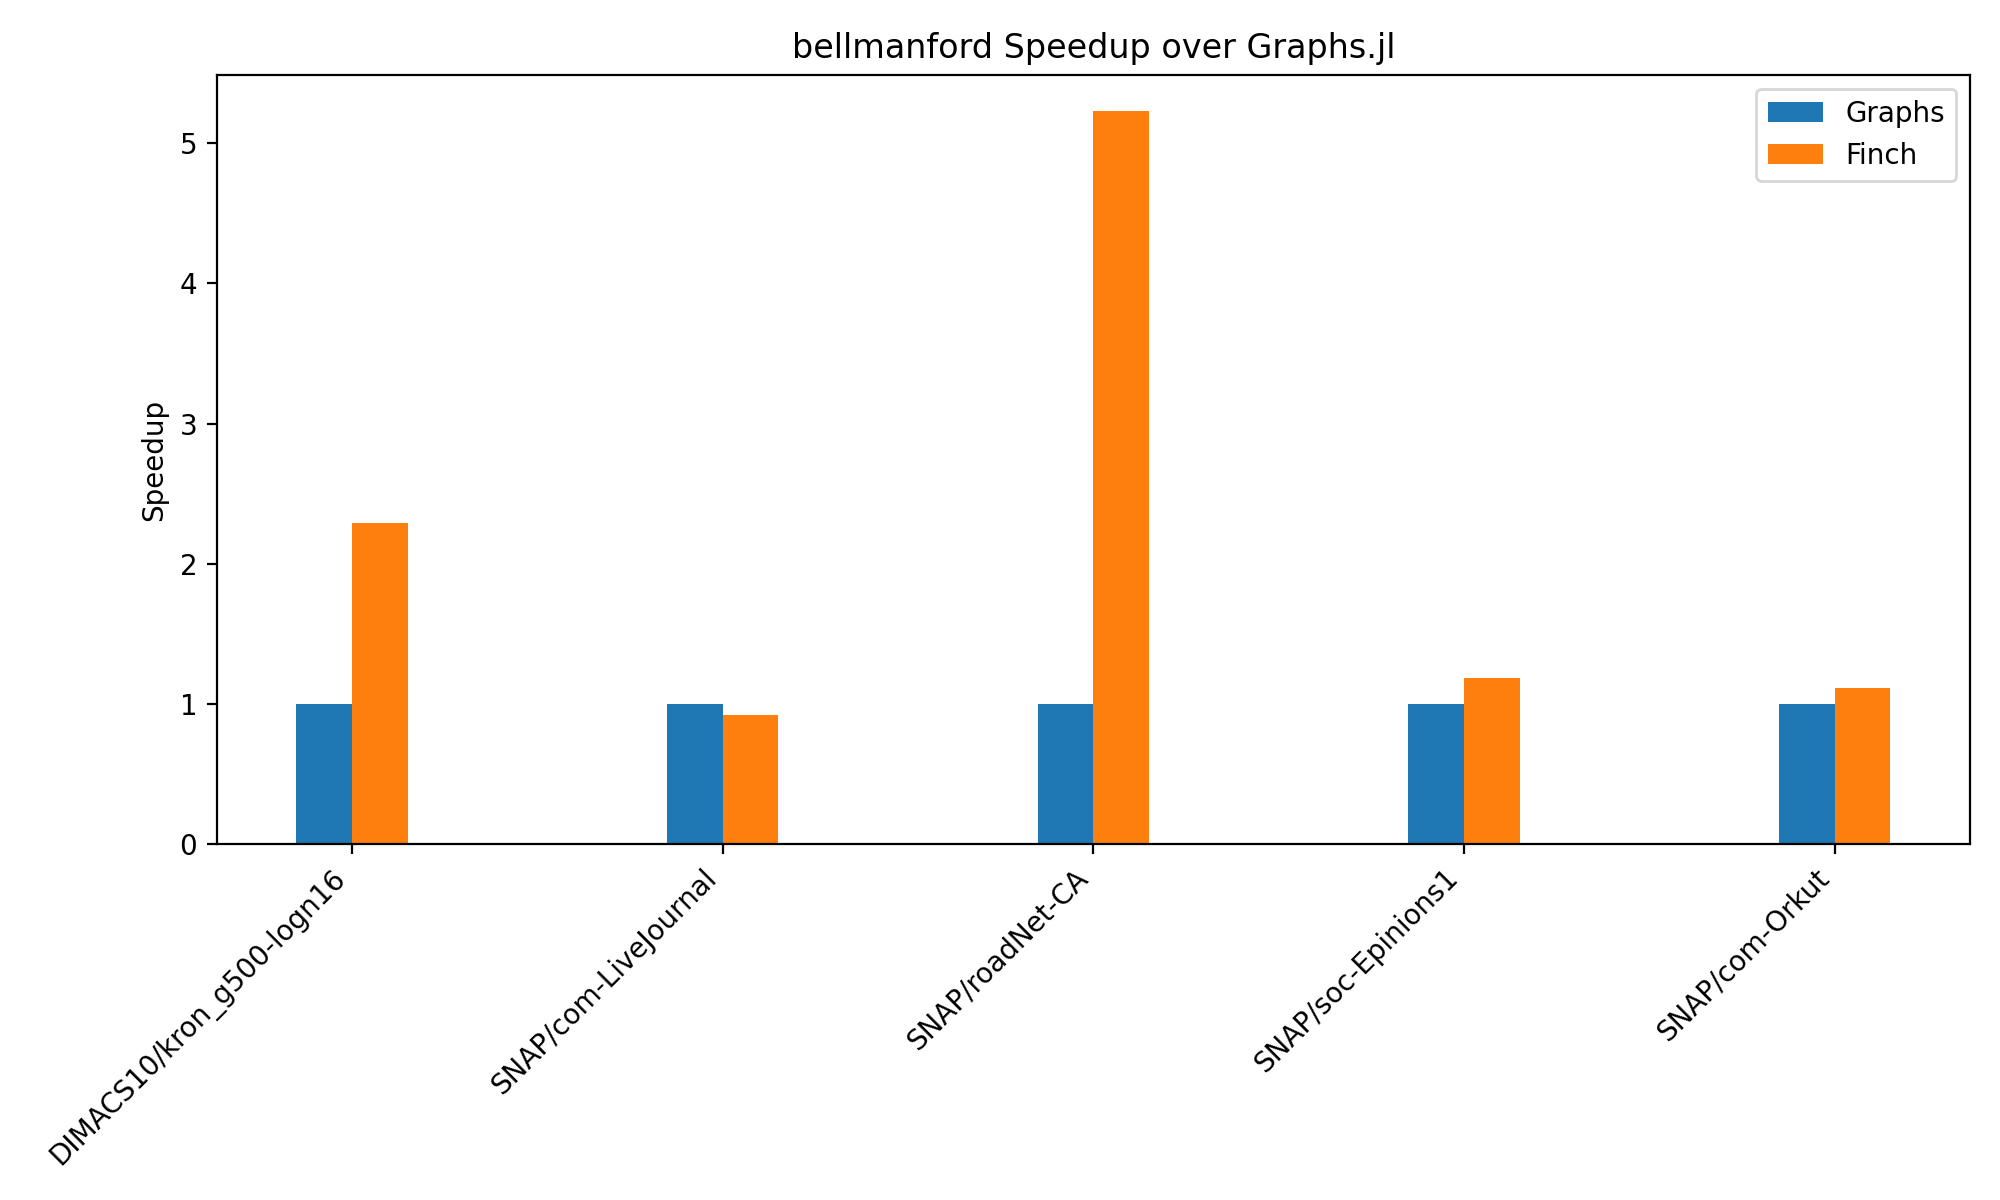
\includegraphics[width=\linewidth]{bellmanford_speedup_over_graphs.jl.png}
    \caption{Performance of graph apps across various tools.}
     \label{graph_result}
\end{figure}

Push-Pull BFS in Finch:
\begin{minted}{julia}
V = Tensor(Dense(Element(false)))
P = Tensor(Dense(Element(0)))
F = Tensor(SparseByteMap(Pattern()))
_F = Tensor(SparseByteMap(Pattern()))
A = Tensor(Dense(SparseList(Pattern())))
AT = Tensor(Dense(SparseList(Pattern())))

function finch_bfs_push_kernel(_F, F, A, V, P)
    @finch begin
        _F .= false
        for j=_, k=_
            if F[j] && A[k, j] && !(V[k])
                _F[k] |= true
                P[k] <<choose(0)>>= j #Only set the parent for this vertex
            end
        end
        return _F
    end
end


function finch_bfs_pull_kernel(_F, F, AT, V, P)
    p = ShortCircuitScalar{0}()
    @finch begin
        _F .= false
        for k=_
            if !V[k]
                p .= 0
                for j=_
                    if F[follow(j)] && AT[j, k]
                        p[] <<choose(0)>>= j #Only set the parent for this vertex
                    end
                end
                if p[] != 0
                    _F[k] |= true
                    P[k] = p[]
                end
            end
        end
        return _F
    end
end
\end{minted}

\subsection{Implementing Numpy's Array API in Finch}
In the past decade, the adoption of the Python Array API \cite{harris_array_2020} has allowed for a proliferation array programming systems, but existing implementations of this API for structured data suffer from either incompleteness or inefficiency. They generally either limit the dimensionality to vectors and matrices or only support tabular representations in order to reduce the complexity of interactions between different formats. Further, existing work doesn't support the fusion of arbitrary operators which can have a drastic impact on performance as we show in Fig. (\kyle{PUT FIG HERE}). We believe that a flexible, online compiler like Finch which can manage the complexity of arbitrary operations between inputs with a wide variety of formats is the secret ingredient needed to make the array API performant for structured data.

There is a gap between the expressiveness of the purely declarative Array API and the Finch language which defines both the output and the algorithm. The naive approach to solving this would be to explicitly define a mapping from each function in the API to a Finch program which eagerly produces the output. This approach results in a simple translation procedure but misses crucial opportunities for optimization across a chain of function calls and needlessly materializes large intermediate results. To avoid this, we have implemented a lazy evaluation approach that collects API calls and then computes output when requested by the user. This is implemented through 1) Finch Logic, a minimal, high-level language for expressing array operations and 2) the Finch Interpreter, which lowers Finch Logic programs to one or more Finch programs while making heuristic decisions about output format, loop ordering, and protocols.

\subsubsection{Finch Logic}
The expression fragment of the logical language takes inspiration from relational algebra while incorporating an ordering on the dimensions of a tensor. This means that every operator (with the exception of $\finchtable$ and $\finchalias$ which are analogous to the scan operator in RA) takes in an indexed tensor and outputs an indexed tensor. Conceptually, an indexed tensor can be thought of as a relation with an ordering on the index attributes and a separate value attribute, and we include the $\finchreorder$ operator to manipulate the order. This ordering is necessary for two reasons 1) the outputs of a function in the Array API must match a defined order on the dimensions based on the order of the inputs' dimensions 2) to benefit from concordant iteration we must ensure that the operands to a mapjoin have compatible index orders.

To express materialization, reuse of common sub-expressions, and multiple outputs, we define queries and plans. A query is the assignment of the output of an expression to a name. We use this assignment to denote that we materialize an expression in memory. Later queries can then access the result of earlier queries through the alias operator which allows multiple queries to benefit from a shared computation. A plan is a sequence of queries and it produces a set of tensors as output. 

\begin{align*}
    \finchplan(queries..., names...) \quad\quad\quad \finchquery(name, expr) \quad\quad\quad \finchreorder(expr, idxs...)\\
     \finchrelabel(expr, idxs...) \quad\quad\quad \finchreformat(expr, format) \quad\quad\quad \finchmapjoin(op, exprs...) \\
    \finchaggregate(op, expr)\quad\quad\quad\quad \finchtable(tns, idxs...)  \quad\quad\quad\quad\quad\quad \finchalias(name) \quad\quad\\
     expr:= \finchreorder | \finchrelabel | \finchreformat |\finchmapjoin | \finchaggregate | \finchtable | \finchalias \quad\quad
\end{align*}

Given this language, we now describe how to define a few example functions from the API as plans in the Finch Logic language. Due to the flexibility of Finch, we can use the custom operators $minby(x,y)$ (which compares $x[1]$ and $y[1]$ and returns the smaller $x$ or $y$) and $tuple(x, y)$ (which returns the tuple $(x,y)$), and we can manipulate an index as a scalar to implement $argmin$. For conciseness, we omit the outer wrapping of $\finchplan(\finchquery(out,...),out)$.
\begin{align*}
&\text{sum}(M, dims=[2]) \rightarrow \finchaggregate(+,\finchrelabel(M, i_1,\ldots,i_d), i_2)\\
&\text{matmul}(A, B) \rightarrow \finchaggregate(+,\finchmapjoin(*, \finchrelabel(A, i, j), \finchrelabel(B, j, k)), j)\\
&\text{argmin}(A, dims=[2]) \rightarrow \finchaggregate(minby,\finchmapjoin(tuple, \finchrelabel(A, i_1,\ldots,i_d), \finchtable(i_2)), i_2)
\end{align*}
Notably, these plans do not specify important details about the computation such as the format of intermediates and the order of the loops. In the following discussion, we provide sensible heuristics and show that they provide good performance on important kernels. However, for larger or more complex programs, it would be important to apply a cost-based optimization strategy which we leave for future work.

\subsubsection{Standardizing \& Heuristic Optimization}
Before a plan in Finch Logic can be interpreted, it must be converted to a standard form which resolves the above questions about loop ordering and output formatting. This standard form has a few syntactic requirements, but the semantically important requirements are 1) all inputs (i.e. tables and alias operators) in a query's RHS must conform to a common ordering of the indices 2) the outermost operator of each query's RHS must be a reformat 3) the expression within the reformat must be a pointwise expression, optionally wrapped in an aggregate operator. The former allows the interpreter to identify the loop order for each kernel. The second determines the output format for each intermediate. The last one guarantees that the innermost expression can be computed as a single kernel.

During the standardization process, a concordization pass is performed which examines each query in order and selects a loop order based on a heuristic which loops over intersecting variables first. Then, each query is examined again and a transposition query is inserted for each input which doesn't match the loop order and then the input is replaced with an alias. At this point, the first semantic requirement is satisfied. Next, a formatting pass is performed which examines each query and selects a level format for each output index based on the formats of the inputs and whether random writes are required. The procedure for this is a simple set of rules which attempts to aggressively preserve the structure present in the input tensors.


\subsubsection{Finch Interpreter} 
Once the Finch Logic program has been converted to the standard form, the Finch Interpreter can execute each query, in order, through a straightforward lowering process. First, the output format is identified by unpacking the outer $\finchreformat$ statement. Next, the inner expression of the is unpacked to identify the aggregate operator and to convert the pointwise expression into a Finch expression. At this point, any aliases to the result of previous queries are replaced with an access to the actual tensor. Lastly, the concordant loop order is identified and instantiated. The lowered query can then be compiled and executed with the Finch compiler, and the result is assigned to $name$ in the plan's scope before proceeding to the next query in the plan. 


\subsubsection{Evaluating Finch Logic}
To demonstrate the performance of Finch Logic, we evaluate it on a series of kernels which benefit from the kind of kernel fusion that it automatically applies; 1) triangle counting on graphs 2) SDDMM 3) multiple elementwise operations. Further, we compare against DuckDB as a state of the art system which implements a form of kernel fusion through pipelined execution and even takes advantage of vector instructions which are not yet present in Finch.


\begin{figure}
	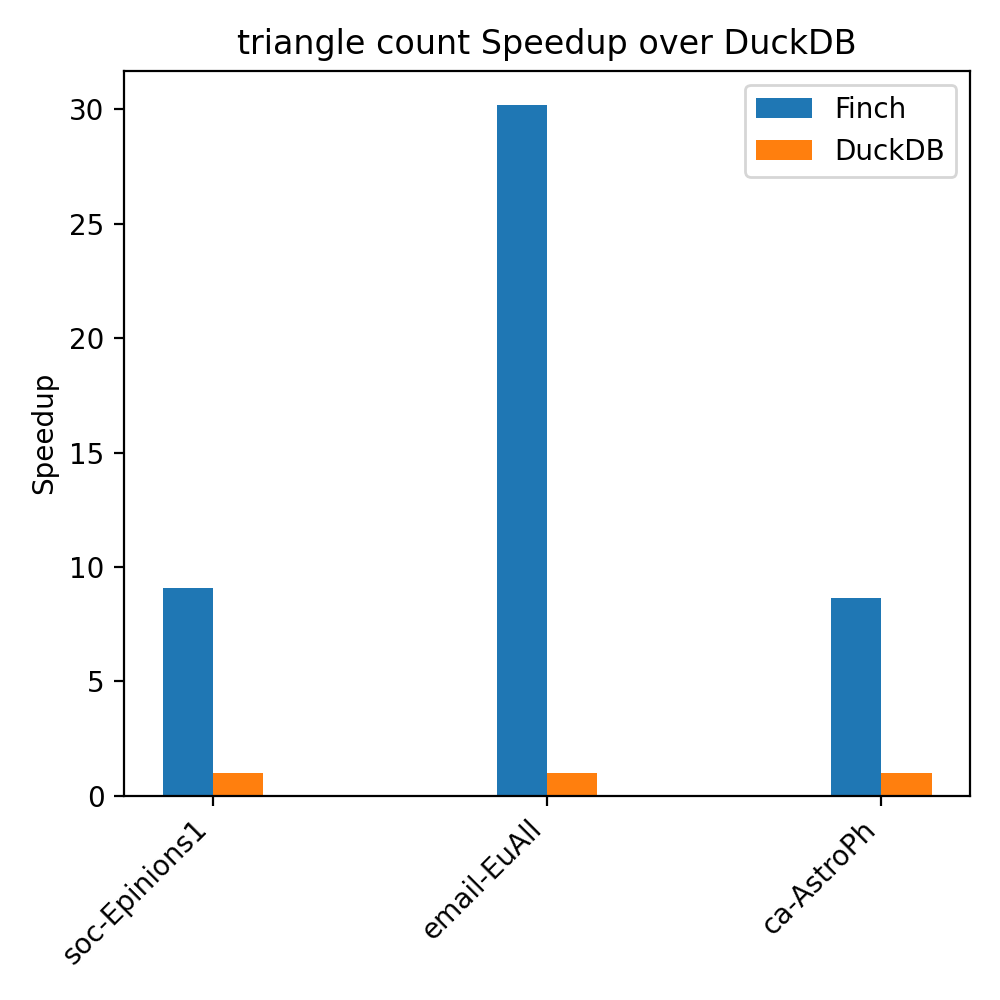
\includegraphics[width=\linewidth]{triangle_count_speedup_over_duckdb.png}
    \caption{Performance of Finch on triangle counting.}
\end{figure}

\begin{figure}
	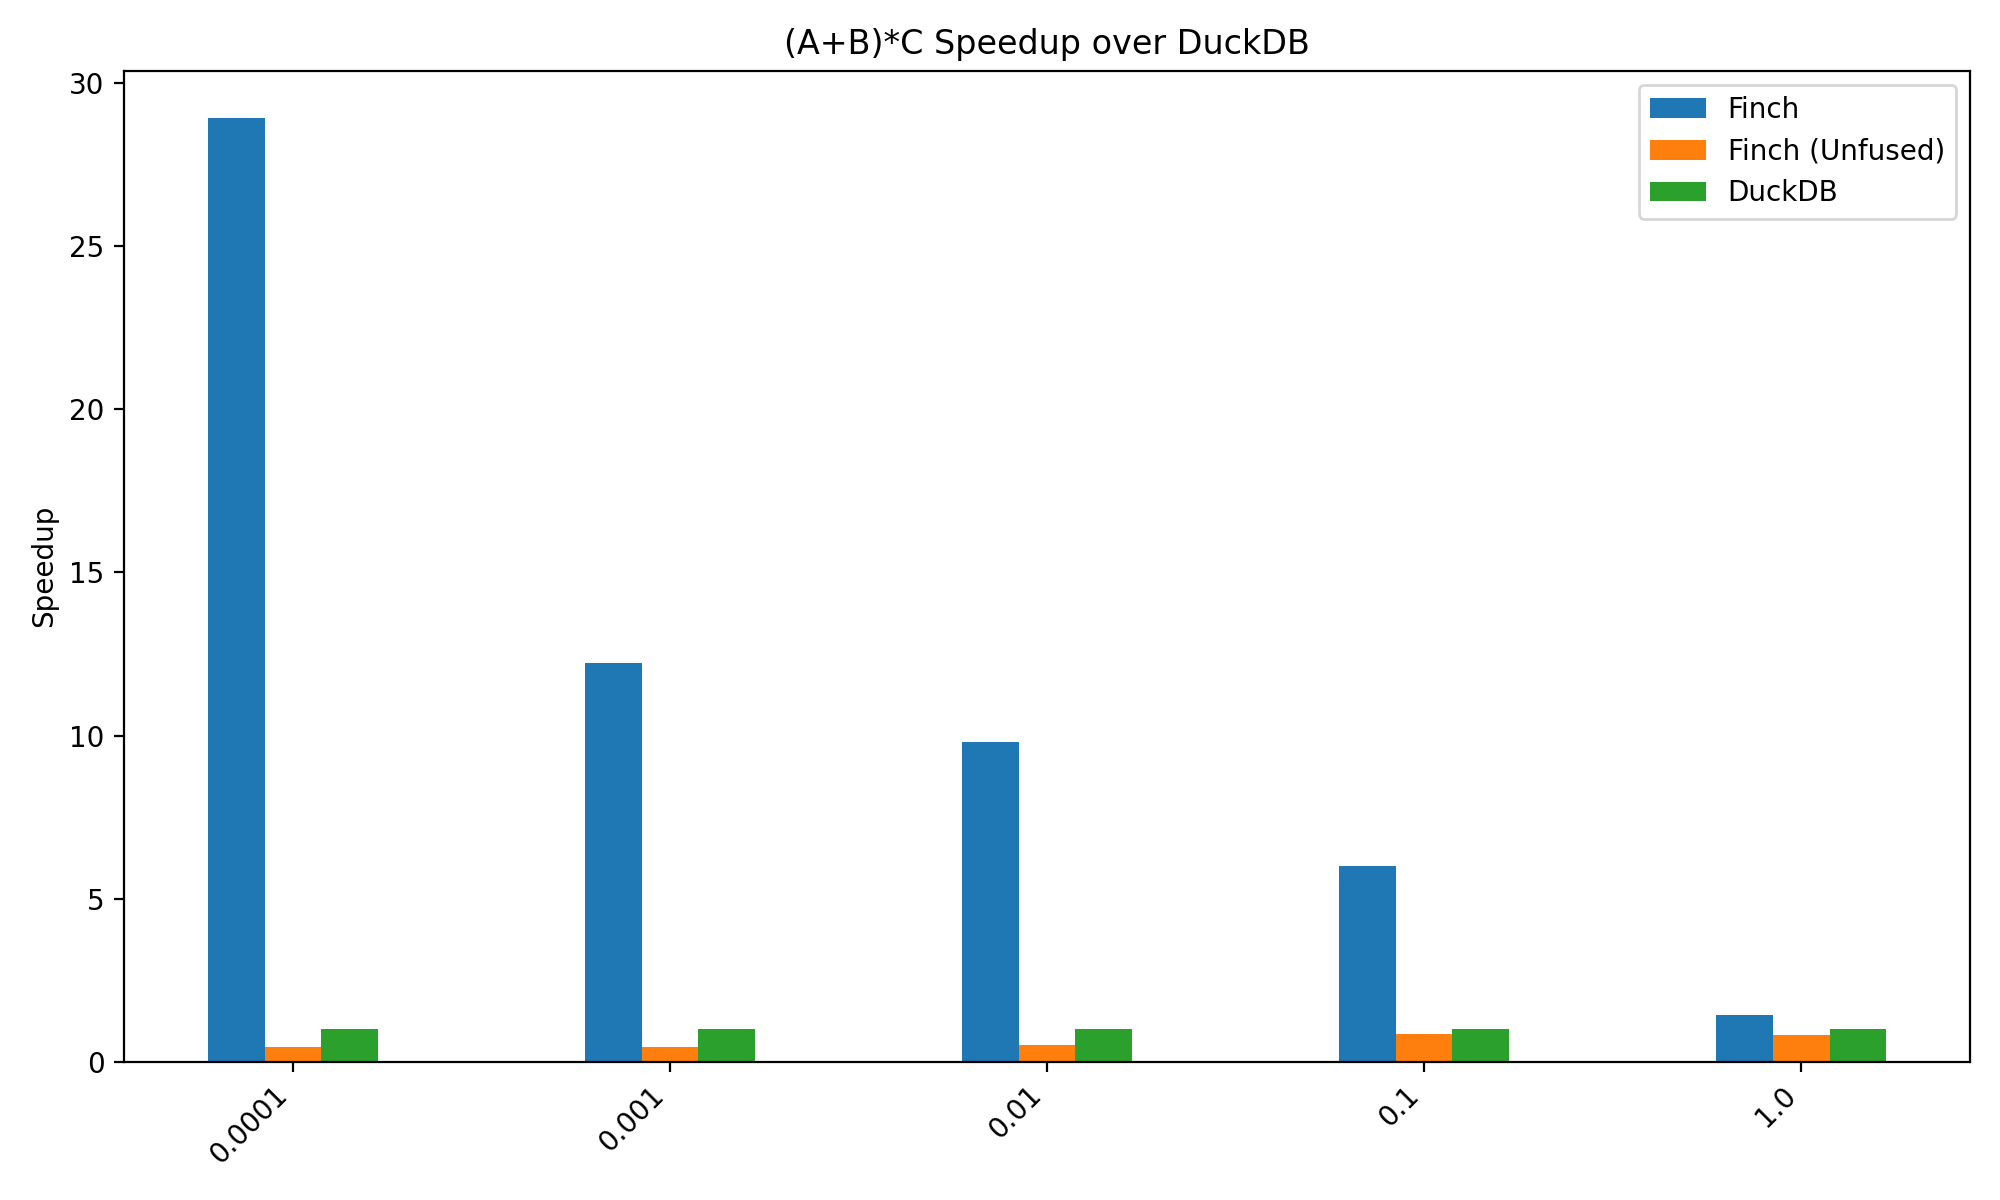
\includegraphics[width=\linewidth]{elementwise_speedup_over_duckdb.png}
    \caption{Performance of Finch on elementwise (A+B)*C kernel as the sparsity of C varies.}
\end{figure}

\begin{figure}
	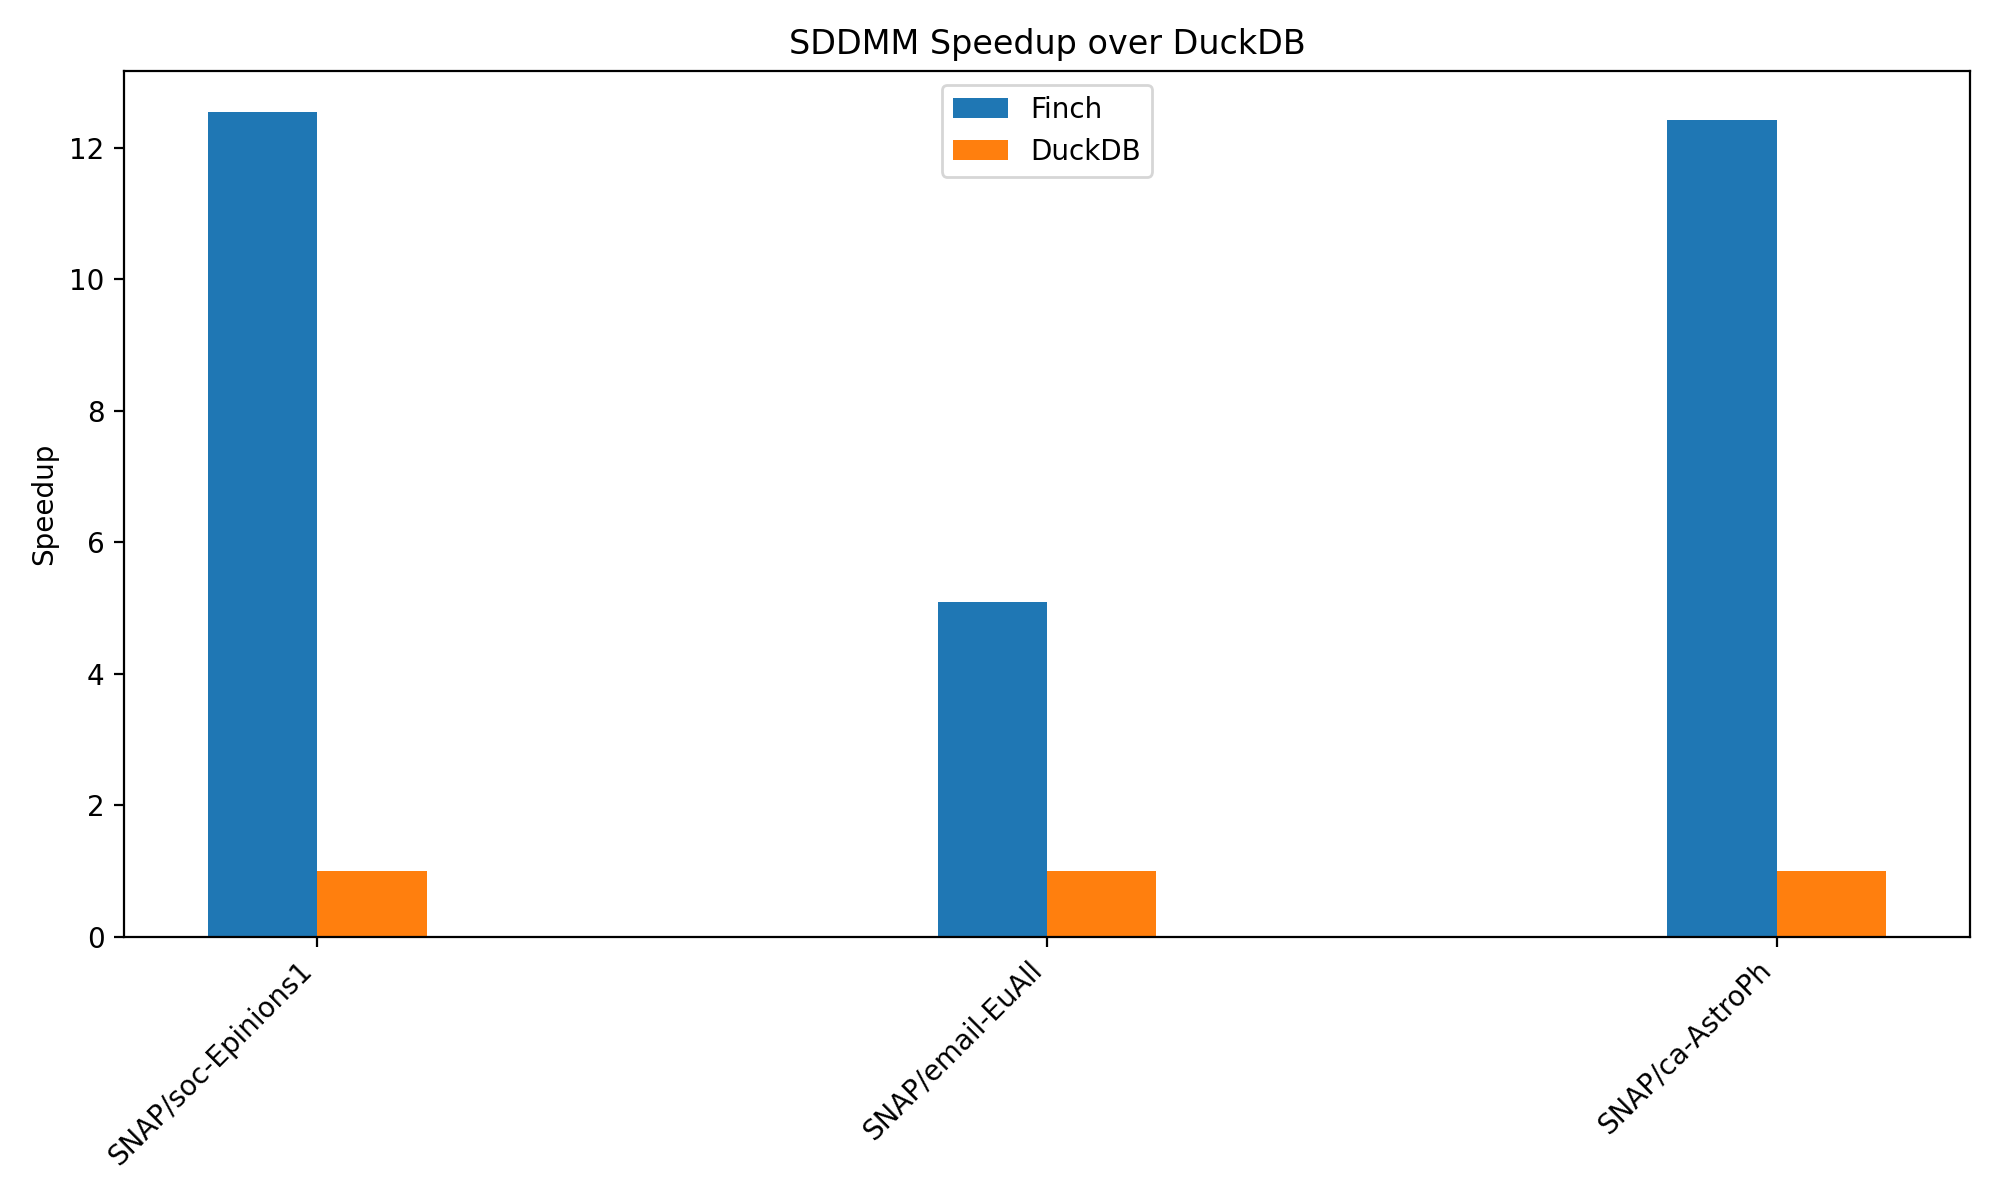
\includegraphics[width=\linewidth]{sddmm_speedup_over_duckdb.png}
    \caption{Performance of Finch on SDDMM.}
\end{figure}



%matmul, mttkrp, repeated ttm, triangle counting, multiple pointwise,
%in-place.
%dot((v^t .* u), w)) vs. 
%(v^t .* dot(u, w))

\willow{Note: I may want to explain format inference somewhere in here, but I'll
have to get to it a little later, perhaps after the paper deadline}
\willow{Note: I think it would be cool to include something about how we support
numerically stable norms and argmin in this model}
\section{Related Work}

The related work on array languages and libraries, both for dense and structured computation, spans several areas.
%
We highlight these works based on if they are a library or language vs. if they are dense or more general.

\paragraph{Dense Libraries:} There are many well known libraries that specialize in dense computations, exemplified by BLAS, though several BLAS routines are specialized to symmetric, hermitian, and triangular matrices~\cite{Anderson1999}.
%
This pattern is carried over into well known dense array libraries that use BLAS, exemplified by Numpy.

\paragraph{Structured Libraries:}

Many libraries support BLAS plus a few sparse array types, typically CSR, CSC, BCSR, and COO.
%
Examples include Scipy, PETSc, Armadillo, and Eigen~\cite{virtanen2020scipy, abhyankarpetsc, Rumengan2021, eigenweb}.
%
Several of these libraries also feature some graph or mesh algorithms built on sparse matrices.
%
GraphBlas exemplifies this pattern with support for many sparse matrix operations on a variety of formats~\cite{kepner2016mathematical} although a variety of other graph libraries adopt a similar approach such as LAgraph or GBase~\cite{mattson2019lagraph, kang2011gbase} among many others.



\paragraph{Dense Tensor Compilers:}

\paragraph{Tensor Compilers for Structured Data:}



%% Libraries: Numpy, LAPACK, blas, graphblas, SplAtt, Scipy, Petsc, Graph libraries (ligraph, lagraph,...)
%% Languages: Halide, Lift, TVM, OptiML
%% Languages: Lgen/Spiral, LAMapping system,
%% languages sparse: TVM Sparse, Tiachi, SPF, TACO, Stut, various extensiosn to TACO, Graphit
%% SQL: HyPer, SDQL + Formats, Vectorwise, Morphesu,

%% Most similar to us: SDQL, SPF Leader Follower, Taichi

\section{Conclusion}
With comprehensive and extensible support for structured data and with the inclusion of control-flow, sparse and structured array programming can be put on the same compiler transformation and code generation footing as dense array codes~\cite{fred-taco}.
%%
%% The acknowledgments section is defined using the "acks" environment
%% (and NOT an unnumbered section). This ensures the proper
%% identification of the section in the article metadata, and the
%% consistent spelling of the heading.
\begin{acks}
    To Mateusz, Hameer, and Jaeyeon for their excellent programming contributions to the Finch codebase.
\end{acks}

%%
%% The next two lines define the bibliography style to be used, and
%% the bibliography file.
\bibliographystyle{ACM-Reference-Format}
\bibliography{FinchOOPSLAWillow.bib, FinchOOPSLAOverleaf.bib}


%%
%% If your work has an appendix, this is the place to put it.
\appendix

\section{SpMV Datasets}


\begin{table}[htbp]
  \centering
  \scriptsize
  \caption{SpMV Sample Matrices}
  \vspace{-12pt}
  \label{tab:spmv_sample_matrices}
  \begin{tabular}{|
      >{\centering\arraybackslash}m{0.2\linewidth-2\tabcolsep-1.2\arrayrulewidth}|
      >{\centering\arraybackslash}m{0.2\linewidth-2\tabcolsep-1.2\arrayrulewidth}|
      >{\centering\arraybackslash}m{0.2\linewidth-2\tabcolsep-1.2\arrayrulewidth}|
      >{\centering\arraybackslash}m{0.2\linewidth-2\tabcolsep-1.2\arrayrulewidth}|
      >{\centering\arraybackslash}m{0.2\linewidth-2\tabcolsep-1.2\arrayrulewidth}|}
      \hline
       & \textbf{HB/saylr4} & \textbf{Norris/heart3} & \textbf{large\_band} & \textbf{SNAP/as-735} \\
      \hline
      \textbf{Spy} & 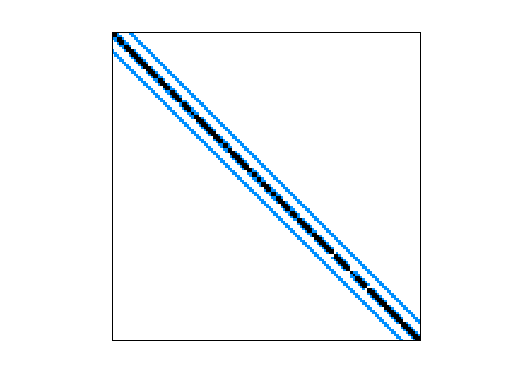
\includegraphics[width=\linewidth]{spmv_matrices/saylr4.png} & 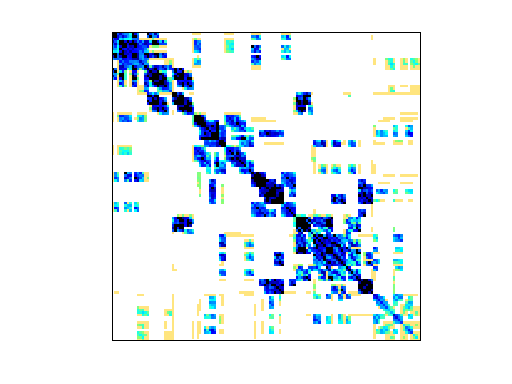
\includegraphics[width=\linewidth]{spmv_matrices/heart3.png} & 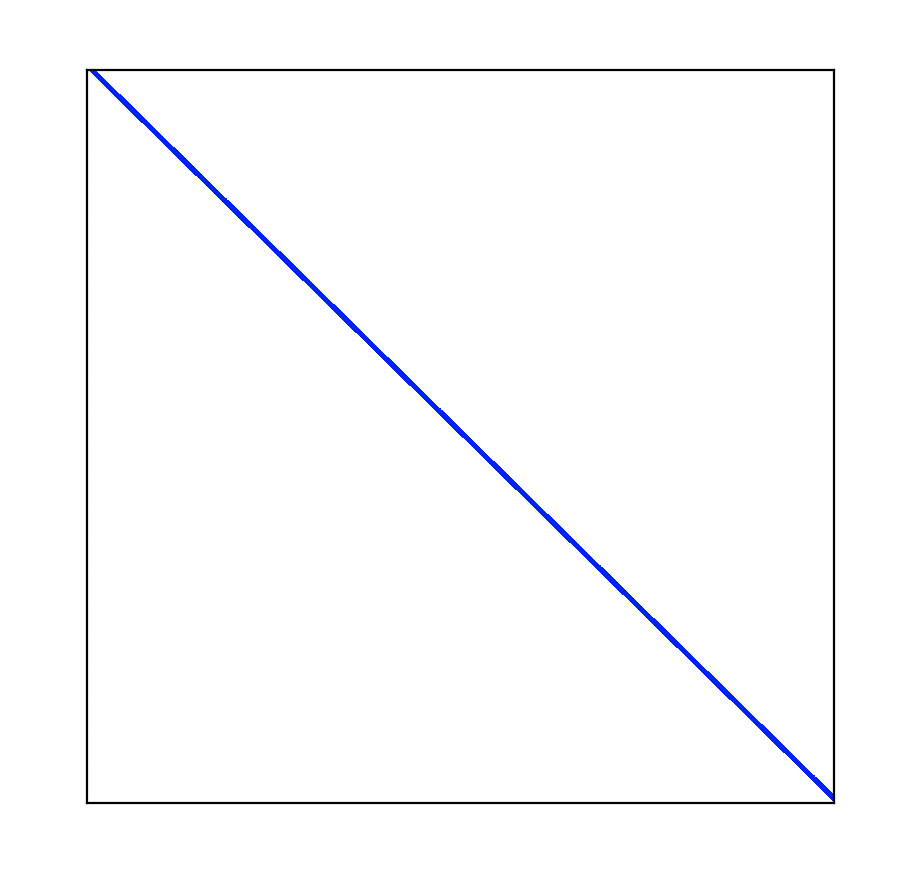
\includegraphics[width=\linewidth]{spmv_matrices/toeplitz_large_band.png} & 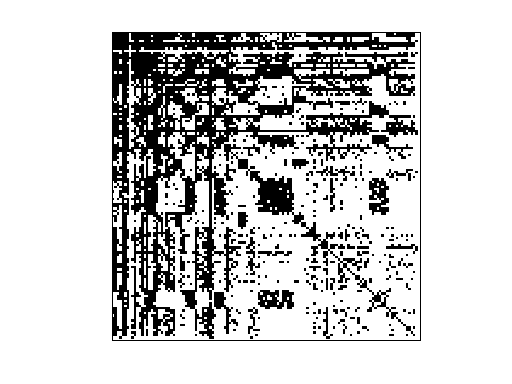
\includegraphics[width=\linewidth]{spmv_matrices/as-735.png} \\
      \hline 
      \textbf{Group / Name} & HB/saylr4 & Norris/heart3 & large\_band & SNAP/as-735 \\
      \hline
      \textbf{Dimensions} & 3,564 x 3,564 (22,316) & 2,339 x 2,339 (680,341) & 10,000 x 10,000 (1,999,900) & 7,716 x 7,716 (26,467) \\
      \hline
      \textbf{Best Finch Format} & Symmetric SparseList & SparseVBL & SparseBand & Symmetric SparseList-Pattern \\
      \hline
  \end{tabular}
  \vspace{-8pt}
\end{table}

\section{Graph Algorithm Listings}\label{sec:graph_listings}

\subsection{Finch Breadth-First Search}
\begin{minted}{julia}
    function bfs_finch_kernel(edges, edgesT, source=5, alpha = 0.01)
    (n, m) = size(edges)
    edges = pattern!(edges)
    @assert n == m
    F = Tensor(SparseByteMap(Pattern()), n)
    _F = Tensor(SparseByteMap(Pattern()), n)
    @finch F[source] = true
    F_nnz = 1 
    V = Tensor(Dense(Element(false)), n)
    @finch V[source] = true
    P = Tensor(Dense(Element(0)), n)
    @finch P[source] = source
    while F_nnz > 0 
        if F_nnz/m > alpha # pull
            p = ShortCircuitScalar{0}()
            _F .= false
            for k=_ 
                if !V[k]
                    p .= 0
                    for j=_ 
                        if F[follow(j)] && AT[j, k]
                            p[] <<choose(0)>>= j
                        end 
                    end 
                    if p[] != 0
                        _F[k] |= true
                        P[k] = p[] 
                    end 
                end 
            end
        else # push
            _F .= false
            for j=_, k=_ 
                if F[j] && A[k, j] && !(V[k])
                    _F[k] |= true
                    P[k] <<choose(0)>>= j
                end 
            end 
        end 
        c = Scalar(0)
        @finch begin
            for k=_ 
                let _f = _F[k]
                    V[k] |= _f
                    c[] += _f
                end 
            end 
        end 
        (F, _F) = (_F, F)
        F_nnz = c[] 
    end 
    return P
end
\end{minted}
\subsection{GraphBLAS Breadth-First Search}
\begin{minted}{c}
//------------------------------------------------------------------------------
// LAGr_BreadthFirstSearch:  breadth-first search dispatch
//------------------------------------------------------------------------------

// LAGraph, (c) 2019-2022 by The LAGraph Contributors, All Rights Reserved.
// SPDX-License-Identifier: BSD-2-Clause
//
// For additional details (including references to third party source code and
// other files) see the LICENSE file or contact permission@sei.cmu.edu. See
// Contributors.txt for a full list of contributors. Created, in part, with
// funding and support from the U.S. Government (see Acknowledgments.txt file).
// DM22-0790

// Contributed by Scott McMillan, SEI Carnegie Mellon University

//------------------------------------------------------------------------------

// Breadth-first-search via push/pull method if using SuiteSparse:GraphBLAS
// and its GxB extensions, or a push-only method otherwise.  The former is
// much faster.

// This is an Advanced algorithm.  SuiteSparse can use a push/pull method if
// G->AT and G->out_degree are provided.  G->AT is not required if G is
// undirected.  The vanilla method is always push-only.

#include "LG_alg_internal.h"

int LAGr_BreadthFirstSearch
(
    // output:
    GrB_Vector *level,
    GrB_Vector *parent,
    // input:
    const LAGraph_Graph G,
    GrB_Index src,
    char *msg
)
{

#if LAGRAPH_SUITESPARSE
    return LG_BreadthFirstSearch_SSGrB   (level, parent, G, src, msg) ;
#else
    return LG_BreadthFirstSearch_vanilla (level, parent, G, src, msg) ;
#endif
}

//------------------------------------------------------------------------------
// LG_BreadthFirstSearch_SSGrB:  BFS using Suitesparse extensions
//------------------------------------------------------------------------------

// LAGraph, (c) 2019-2022 by The LAGraph Contributors, All Rights Reserved.
// SPDX-License-Identifier: BSD-2-Clause
//
// For additional details (including references to third party source code and
// other files) see the LICENSE file or contact permission@sei.cmu.edu. See
// Contributors.txt for a full list of contributors. Created, in part, with
// funding and support from the U.S. Government (see Acknowledgments.txt file).
// DM22-0790

// Contributed by Timothy A. Davis, Texas A&M University

//------------------------------------------------------------------------------

// This is an Advanced algorithm.  G->AT and G->out_degree are required for
// this method to use push-pull optimization.  If not provided, this method
// defaults to a push-only algorithm, which can be slower.  This is not
// user-callable (see LAGr_BreadthFirstSearch instead).  G->AT and
// G->out_degree are not computed if not present.

// References:
//
// Carl Yang, Aydin Buluc, and John D. Owens. 2018. Implementing Push-Pull
// Efficiently in GraphBLAS. In Proceedings of the 47th International
// Conference on Parallel Processing (ICPP 2018). ACM, New York, NY, USA,
// Article 89, 11 pages. DOI: https://doi.org/10.1145/3225058.3225122
//
// Scott Beamer, Krste Asanovic and David A. Patterson, The GAP Benchmark
// Suite, http://arxiv.org/abs/1508.03619, 2015.  http://gap.cs.berkeley.edu/

// revised by Tim Davis (davis@tamu.edu), Texas A&M University

#define LG_FREE_WORK        \
{                           \
    GrB_free (&w) ;         \
    GrB_free (&q) ;         \
}

#define LG_FREE_ALL         \
{                           \
    LG_FREE_WORK ;          \
    GrB_free (&pi) ;        \
    GrB_free (&v) ;         \
}

#include "LG_internal.h"

int LG_BreadthFirstSearch_SSGrB
(
    GrB_Vector *level,
    GrB_Vector *parent,
    const LAGraph_Graph G,
    GrB_Index src,
    char *msg
)
{

    //--------------------------------------------------------------------------
    // check inputs
    //--------------------------------------------------------------------------

    LG_CLEAR_MSG ;
    GrB_Vector q = NULL ;           // the current frontier
    GrB_Vector w = NULL ;           // to compute work remaining
    GrB_Vector pi = NULL ;          // parent vector
    GrB_Vector v = NULL ;           // level vector

#if !LAGRAPH_SUITESPARSE
    LG_ASSERT (false, GrB_NOT_IMPLEMENTED) ;
#else

    bool compute_level  = (level != NULL) ;
    bool compute_parent = (parent != NULL) ;
    if (compute_level ) (*level ) = NULL ;
    if (compute_parent) (*parent) = NULL ;
    LG_ASSERT_MSG (compute_level || compute_parent, GrB_NULL_POINTER,
        "either level or parent must be non-NULL") ;

    LG_TRY (LAGraph_CheckGraph (G, msg)) ;

    //--------------------------------------------------------------------------
    // get the problem size and cached properties
    //--------------------------------------------------------------------------

    GrB_Matrix A = G->A ;

    GrB_Index n, nvals ;
    GRB_TRY (GrB_Matrix_nrows (&n, A)) ;
    LG_ASSERT_MSG (src < n, GrB_INVALID_INDEX, "invalid source node") ;

    GRB_TRY (GrB_Matrix_nvals (&nvals, A)) ;

    GrB_Matrix AT = NULL ;
    GrB_Vector Degree = G->out_degree ;
    if (G->kind == LAGraph_ADJACENCY_UNDIRECTED ||
       (G->kind == LAGraph_ADJACENCY_DIRECTED &&
        G->is_symmetric_structure == LAGraph_TRUE))
    {
        // AT and A have the same structure and can be used in both directions
        AT = G->A ;
    }
    else
    {
        // AT = A' is different from A.  If G->AT is NULL, then a push-only
        // method is used.
        AT = G->AT ;
    }

    // direction-optimization requires G->AT (if G is directed) and
    // G->out_degree (for both undirected and directed cases)
    bool push_pull = (Degree != NULL && AT != NULL) ;

    // determine the semiring type
    GrB_Type int_type = (n > INT32_MAX) ? GrB_INT64 : GrB_INT32 ;
    GrB_Semiring semiring ;

    if (compute_parent)
    {
        // use the ANY_SECONDI_INT* semiring: either 32 or 64-bit depending on
        // the # of nodes in the graph.
        semiring = (n > INT32_MAX) ?
            GxB_ANY_SECONDI_INT64 : GxB_ANY_SECONDI_INT32 ;

        // create the parent vector.  pi(i) is the parent id of node i
        GRB_TRY (GrB_Vector_new (&pi, int_type, n)) ;
        GRB_TRY (GxB_set (pi, GxB_SPARSITY_CONTROL, GxB_BITMAP + GxB_FULL)) ;
        // pi (src) = src denotes the root of the BFS tree
        GRB_TRY (GrB_Vector_setElement (pi, src, src)) ;

        // create a sparse integer vector q, and set q(src) = src
        GRB_TRY (GrB_Vector_new (&q, int_type, n)) ;
        GRB_TRY (GrB_Vector_setElement (q, src, src)) ;
    }
    else
    {
        // only the level is needed, use the LAGraph_any_one_bool semiring
        semiring = LAGraph_any_one_bool ;

        // create a sparse boolean vector q, and set q(src) = true
        GRB_TRY (GrB_Vector_new (&q, GrB_BOOL, n)) ;
        GRB_TRY (GrB_Vector_setElement (q, true, src)) ;
    }

    if (compute_level)
    {
        // create the level vector. v(i) is the level of node i
        // v (src) = 0 denotes the source node
        GRB_TRY (GrB_Vector_new (&v, int_type, n)) ;
        GRB_TRY (GxB_set (v, GxB_SPARSITY_CONTROL, GxB_BITMAP + GxB_FULL)) ;
        GRB_TRY (GrB_Vector_setElement (v, 0, src)) ;
    }

    // workspace for computing work remaining
    GRB_TRY (GrB_Vector_new (&w, GrB_INT64, n)) ;

    GrB_Index nq = 1 ;          // number of nodes in the current level
    double alpha = 8.0 ;
    double beta1 = 8.0 ;
    double beta2 = 512.0 ;
    int64_t n_over_beta1 = (int64_t) (((double) n) / beta1) ;
    int64_t n_over_beta2 = (int64_t) (((double) n) / beta2) ;

    //--------------------------------------------------------------------------
    // BFS traversal and label the nodes
    //--------------------------------------------------------------------------

    bool do_push = true ;       // start with push
    GrB_Index last_nq = 0 ;
    int64_t edges_unexplored = nvals ;
    bool any_pull = false ;     // true if any pull phase has been done

    // {!mask} is the set of unvisited nodes
    GrB_Vector mask = (compute_parent) ? pi : v ;

    for (int64_t nvisited = 1, k = 1 ; nvisited < n ; nvisited += nq, k++)
    {

        //----------------------------------------------------------------------
        // select push vs pull
        //----------------------------------------------------------------------

        if (push_pull)
        {
            if (do_push)
            {
                // check for switch from push to pull
                bool growing = nq > last_nq ;
                bool switch_to_pull = false ;
                if (edges_unexplored < n)
                {
                    // very little of the graph is left; disable the pull
                    push_pull = false ;
                }
                else if (any_pull)
                {
                    // once any pull phase has been done, the # of edges in the
                    // frontier has no longer been tracked.  But now the BFS
                    // has switched back to push, and we're checking for yet
                    // another switch to pull.  This switch is unlikely, so
                    // just keep track of the size of the frontier, and switch
                    // if it starts growing again and is getting big.
                    switch_to_pull = (growing && nq > n_over_beta1) ;
                }
                else
                {
                    // update the # of unexplored edges
                    // w<q>=Degree
                    // w(i) = outdegree of node i if node i is in the queue
                    GRB_TRY (GrB_assign (w, q, NULL, Degree, GrB_ALL, n,
                        GrB_DESC_RS)) ;
                    // edges_in_frontier = sum (w) = # of edges incident on all
                    // nodes in the current frontier
                    int64_t edges_in_frontier = 0 ;
                    GRB_TRY (GrB_reduce (&edges_in_frontier, NULL,
                        GrB_PLUS_MONOID_INT64, w, NULL)) ;
                    edges_unexplored -= edges_in_frontier ;
                    switch_to_pull = growing &&
                        (edges_in_frontier > (edges_unexplored / alpha)) ;
                }
                if (switch_to_pull)
                {
                    // switch from push to pull
                    do_push = false ;
                }
            }
            else
            {
                // check for switch from pull to push
                bool shrinking = nq < last_nq ;
                if (shrinking && (nq <= n_over_beta2))
                {
                    // switch from pull to push
                    do_push = true ;
                }
            }
            any_pull = any_pull || (!do_push) ;
        }

        //----------------------------------------------------------------------
        // q = kth level of the BFS
        //----------------------------------------------------------------------

        int sparsity = do_push ? GxB_SPARSE : GxB_BITMAP ;
        GRB_TRY (GxB_set (q, GxB_SPARSITY_CONTROL, sparsity)) ;

        // mask is pi if computing parent, v if computing just level
        if (do_push)
        {
            // push (saxpy-based vxm):  q'{!mask} = q'*A
            GRB_TRY (GrB_vxm (q, mask, NULL, semiring, q, A, GrB_DESC_RSC)) ;
        }
        else
        {
            // pull (dot-product-based mxv):  q{!mask} = AT*q
            GRB_TRY (GrB_mxv (q, mask, NULL, semiring, AT, q, GrB_DESC_RSC)) ;
        }

        //----------------------------------------------------------------------
        // done if q is empty
        //----------------------------------------------------------------------

        last_nq = nq ;
        GRB_TRY (GrB_Vector_nvals (&nq, q)) ;
        if (nq == 0)
        {
            break ;
        }

        //----------------------------------------------------------------------
        // assign parents/levels
        //----------------------------------------------------------------------

        if (compute_parent)
        {
            // q(i) currently contains the parent id of node i in tree.
            // pi{q} = q
            GRB_TRY (GrB_assign (pi, q, NULL, q, GrB_ALL, n, GrB_DESC_S)) ;
        }
        if (compute_level)
        {
            // v{q} = k, the kth level of the BFS
            GRB_TRY (GrB_assign (v, q, NULL, k, GrB_ALL, n, GrB_DESC_S)) ;
        }
    }

    //--------------------------------------------------------------------------
    // free workspace and return result
    //--------------------------------------------------------------------------

    if (compute_parent) (*parent) = pi ;
    if (compute_level ) (*level ) = v ;
    LG_FREE_WORK ;
    return (GrB_SUCCESS) ;
#endif
}
\end{minted}
\subsection{Finch Bellman-Ford}
\begin{minted}{julia}
function bellmanford_finch_kernel(edges, source=1)
    (n, m) = size(edges)
    @assert n == m
    dists_prev = Tensor(Dense(Element(Inf)), n)
    dists_prev[source] = 0 
    dists = Tensor(Dense(Element(Inf)), n)
    active_prev = Tensor(SparseByteMap(Pattern()), n)
    active_prev[source] = true
    active = Tensor(SparseByteMap(Pattern()), n)
    parents = Tensor(Dense(Element(0)), n)
    for iter = 1:n  
        @finch begin
            for j=_ 
                if active_prev[j]
                    dists[j] <<min>>= dists_prev[j]
                end 
            end 
        end 
        @finch begin
            active .= false
            for j = _ 
                if active_prev[j]
                    for i = _ 
                        let d = dists_prev[j] + edges[i, j]
                            dists[i] <<min>>= d
                            active[i] |= d < dists_prev[i]
                        end 
                    end 
                end 
            end 
        end 
        if countstored(active) == 0
            break
        end 
        dists_prev, dists = dists, dists_prev
        active_prev, active = active, active_prev
    end 
    @finch begin
        for j = _ 
            for i = _ 
                let d = edges[i, j]
                    if d < Inf && dists[j] + d <= dists[i]
                        parents[i] <<choose(0)>>= j
                    end 
                end 
            end 
        end 
    end 
    return (dists=dists, parents=parents)
end
\end{minted}

\subsection{GraphBLAS Bellman-Ford}
\begin{minted}{c}
//------------------------------------------------------------------------------
// LAGraph_BF_full1a.c: Bellman-Ford single-source shortest paths, returns tree,
// while diagonal of input matrix A needs not to be explicit 0
//------------------------------------------------------------------------------

// LAGraph, (c) 2019-2022 by The LAGraph Contributors, All Rights Reserved.
// SPDX-License-Identifier: BSD-2-Clause
//
// For additional details (including references to third party source code and
// other files) see the LICENSE file or contact permission@sei.cmu.edu. See
// Contributors.txt for a full list of contributors. Created, in part, with
// funding and support from the U.S. Government (see Acknowledgments.txt file).
// DM22-0790

// Contributed by Jinhao Chen and Timothy A. Davis, Texas A&M University

//------------------------------------------------------------------------------

// This is the fastest variant that computes both the parent & the path length.

// LAGraph_BF_full1a: Bellman-Ford single source shortest paths, returning both
// the path lengths and the shortest-path tree.

// LAGraph_BF_full performs a Bellman-Ford to find out shortest path, parent
// nodes along the path and the hops (number of edges) in the path from given
// source vertex s in the range of [0, n) on graph given as matrix A with size
// n*n. The sparse matrix A has entry A(i, j) if there is an edge from vertex i
// to vertex j with weight w, then A(i, j) = w.

// LAGraph_BF_full1a returns GrB_SUCCESS if it succeeds.  In this case, there
// are no negative-weight cycles in the graph, and d, pi, and h are returned.
// The vector d has d(k) as the shortest distance from s to k. pi(k) = p+1,
// where p is the parent node of k-th node in the shortest path. In particular,
// pi(s) = 0. h(k) = hop(s, k), the number of edges from s to k in the shortest
// path.

// If the graph has a negative-weight cycle, GrB_NO_VALUE is returned, and the
// GrB_Vectors d(k), pi(k) and h(k)  (i.e., *pd_output, *ppi_output and
// *ph_output respectively) will be NULL when negative-weight cycle detected.

// Otherwise, other errors such as GrB_OUT_OF_MEMORY, GrB_INVALID_OBJECT, and
// so on, can be returned, if these errors are found by the underlying
// GrB_* functions.

//------------------------------------------------------------------------------

#define LG_FREE_WORK                   \
{                                      \
    GrB_free(&d);                      \
    GrB_free(&dmasked);                \
    GrB_free(&dless);                  \
    GrB_free(&Atmp);                   \
    GrB_free(&BF_Tuple3);              \
    GrB_free(&BF_lMIN_Tuple3);         \
    GrB_free(&BF_PLUSrhs_Tuple3);      \
    GrB_free(&BF_LT_Tuple3);           \
    GrB_free(&BF_lMIN_Tuple3_Monoid);  \
    GrB_free(&BF_lMIN_PLUSrhs_Tuple3); \
    LAGraph_Free ((void**)&I, NULL);   \
    LAGraph_Free ((void**)&J, NULL);   \
    LAGraph_Free ((void**)&w, NULL);   \
    LAGraph_Free ((void**)&W, NULL);   \
    LAGraph_Free ((void**)&h, NULL);   \
    LAGraph_Free ((void**)&pi, NULL);  \
}

#define LG_FREE_ALL                    \
{                                      \
    LG_FREE_WORK ;                     \
    GrB_free (pd_output);              \
    GrB_free (ppi_output);             \
    GrB_free (ph_output);              \
}

#include <LAGraph.h>
#include <LAGraphX.h>
#include <LG_internal.h>  // from src/utility

typedef void (*LAGraph_binary_function) (void *, const void *, const void *) ;

//------------------------------------------------------------------------------
// data type for each entry of the adjacent matrix A and "distance" vector d;
// <INFINITY,INFINITY,INFINITY> corresponds to nonexistence of a path, and
// the value  <0, 0, NULL> corresponds to a path from a vertex to itself
//------------------------------------------------------------------------------

typedef struct
{
    double w;    // w  corresponds to a path weight.
    GrB_Index h; // h  corresponds to a path size or number of hops.
    GrB_Index pi;// pi corresponds to the penultimate vertex along a path.
                 // vertex indexed as 1, 2, 3, ... , V, and pi = 0 (as nil)
                 // for u=v, and pi = UINT64_MAX (as inf) for (u,v) not in E
}
BF_Tuple3_struct;

//------------------------------------------------------------------------------
// binary functions, z=f(x,y), where Tuple3xTuple3 -> Tuple3
//------------------------------------------------------------------------------

void BF_lMIN3
(
    BF_Tuple3_struct *z,
    const BF_Tuple3_struct *x,
    const BF_Tuple3_struct *y
)
{
    if (x->w < y->w
        || (x->w == y->w && x->h < y->h)
        || (x->w == y->w && x->h == y->h && x->pi < y->pi))
    {
        if (z != x) { *z = *x; }
    }
    else
    {
        *z = *y;
    }
}

void BF_PLUSrhs3
(
    BF_Tuple3_struct *z,
    const BF_Tuple3_struct *x,
    const BF_Tuple3_struct *y
)
{
    z->w = x->w + y->w ;
    z->h = x->h + y->h ;
    z->pi = (x->pi != UINT64_MAX && y->pi != 0) ?  y->pi : x->pi ;
}

void BF_LT3
(
    bool *z,
    const BF_Tuple3_struct *x,
    const BF_Tuple3_struct *y
)
{
    (*z) = (x->w < y->w
        || (x->w == y->w && x->h < y->h)
        || (x->w == y->w && x->h == y->h && x->pi < y->pi)) ;
}

// Given a n-by-n adjacency matrix A and a source vertex s.
// If there is no negative-weight cycle reachable from s, return the distances
// of shortest paths from s and parents along the paths as vector d. Otherwise,
// returns d=NULL if there is a negtive-weight cycle.
// pd_output is pointer to a GrB_Vector, where the i-th entry is d(s,i), the
//   sum of edges length in the shortest path
// ppi_output is pointer to a GrB_Vector, where the i-th entry is pi(i), the
//   parent of i-th vertex in the shortest path
// ph_output is pointer to a GrB_Vector, where the i-th entry is h(s,i), the
//   number of edges from s to i in the shortest path
// A has weights on corresponding entries of edges
// s is given index for source vertex
GrB_Info LAGraph_BF_full1a
(
    GrB_Vector *pd_output,      //the pointer to the vector of distance
    GrB_Vector *ppi_output,     //the pointer to the vector of parent
    GrB_Vector *ph_output,      //the pointer to the vector of hops
    const GrB_Matrix A,         //matrix for the graph
    const GrB_Index s           //given index of the source
)
{
    GrB_Info info;
    char *msg = NULL ;
    // tmp vector to store distance vector after n (i.e., V) loops
    GrB_Vector d = NULL, dmasked = NULL, dless = NULL;
    GrB_Matrix Atmp = NULL;
    GrB_Type BF_Tuple3;

    GrB_BinaryOp BF_lMIN_Tuple3;
    GrB_BinaryOp BF_PLUSrhs_Tuple3;
    GrB_BinaryOp BF_LT_Tuple3;

    GrB_Monoid BF_lMIN_Tuple3_Monoid;
    GrB_Semiring BF_lMIN_PLUSrhs_Tuple3;

    GrB_Index nrows, ncols, n, nz;  // n = # of row/col, nz = # of nnz in graph
    GrB_Index *I = NULL, *J = NULL; // for col/row indices of entries from A
    GrB_Index *h = NULL, *pi = NULL;
    double *w = NULL;
    BF_Tuple3_struct *W = NULL;

    if (pd_output  != NULL) *pd_output  = NULL;
    if (ppi_output != NULL) *ppi_output = NULL;
    if (ph_output  != NULL) *ph_output  = NULL;

    LG_ASSERT (A != NULL && pd_output != NULL &&
        ppi_output != NULL && ph_output != NULL, GrB_NULL_POINTER) ;

    GRB_TRY (GrB_Matrix_nrows (&nrows, A)) ;
    GRB_TRY (GrB_Matrix_ncols (&ncols, A)) ;
    GRB_TRY (GrB_Matrix_nvals (&nz, A));
    LG_ASSERT_MSG (nrows == ncols, -1002, "A must be square") ;
    n = nrows;
    LG_ASSERT_MSG (s < n, GrB_INVALID_INDEX, "invalid source node") ;

    //--------------------------------------------------------------------------
    // create all GrB_Type GrB_BinaryOp GrB_Monoid and GrB_Semiring
    //--------------------------------------------------------------------------
    // GrB_Type
    GRB_TRY (GrB_Type_new(&BF_Tuple3, sizeof(BF_Tuple3_struct)));

    // GrB_BinaryOp
    GRB_TRY (GrB_BinaryOp_new(&BF_LT_Tuple3,
        (LAGraph_binary_function) (&BF_LT3), GrB_BOOL, BF_Tuple3, BF_Tuple3));
    GRB_TRY (GrB_BinaryOp_new(&BF_lMIN_Tuple3,
        (LAGraph_binary_function) (&BF_lMIN3), BF_Tuple3, BF_Tuple3,BF_Tuple3));
    GRB_TRY (GrB_BinaryOp_new(&BF_PLUSrhs_Tuple3,
        (LAGraph_binary_function)(&BF_PLUSrhs3),
        BF_Tuple3, BF_Tuple3, BF_Tuple3));

    // GrB_Monoid
    BF_Tuple3_struct BF_identity = (BF_Tuple3_struct) { .w = INFINITY,
        .h = UINT64_MAX, .pi = UINT64_MAX };
    GRB_TRY (GrB_Monoid_new_UDT(&BF_lMIN_Tuple3_Monoid, BF_lMIN_Tuple3,
        &BF_identity));

    //GrB_Semiring
    GRB_TRY (GrB_Semiring_new(&BF_lMIN_PLUSrhs_Tuple3,
        BF_lMIN_Tuple3_Monoid, BF_PLUSrhs_Tuple3));

    //--------------------------------------------------------------------------
    // allocate arrays used for tuplets
    //--------------------------------------------------------------------------
#if 1
    LAGRAPH_TRY (LAGraph_Malloc ((void **) &I, nz, sizeof(GrB_Index), msg)) ;
    LAGRAPH_TRY (LAGraph_Malloc ((void **) &J, nz, sizeof(GrB_Index), msg)) ;
    LAGRAPH_TRY (LAGraph_Malloc ((void **) &w, nz, sizeof(double), msg)) ;
    LAGRAPH_TRY (LAGraph_Malloc ((void **) &W, nz, sizeof(BF_Tuple3_struct),
        msg)) ;

    //--------------------------------------------------------------------------
    // create matrix Atmp based on A, while its entries become BF_Tuple3 type
    //--------------------------------------------------------------------------

    GRB_TRY (GrB_Matrix_extractTuples_FP64(I, J, w, &nz, A));
    int nthreads, nthreads_outer, nthreads_inner ;
    LG_TRY (LAGraph_GetNumThreads (&nthreads_outer, &nthreads_inner, msg)) ;
    nthreads = nthreads_outer * nthreads_inner ;
    printf ("nthreads %d\n", nthreads) ;
    int64_t k;
    #pragma omp parallel for num_threads(nthreads) schedule(static)
    for (k = 0; k < nz; k++)
    {
        W[k] = (BF_Tuple3_struct) { .w = w[k], .h = 1, .pi = I[k] + 1 };
    }
    GRB_TRY (GrB_Matrix_new(&Atmp, BF_Tuple3, n, n));
    GRB_TRY (GrB_Matrix_build_UDT(Atmp, I, J, W, nz, BF_lMIN_Tuple3));
    LAGraph_Free ((void**)&I, NULL);
    LAGraph_Free ((void**)&J, NULL);
    LAGraph_Free ((void**)&W, NULL);
    LAGraph_Free ((void**)&w, NULL);

#else

    todo: GraphBLAS could use a new kind of unary operator, not z=f(x), but

    [z,flag] = f (aij, i, j, k, nrows, ncols, nvals, etc, ...)
    flag: keep or discard.  Combines GrB_apply and GxB_select.

    builtins:
        f(...) =
            i, bool is true
            j, bool is true
            i+j*nrows, etc.
            k
            tril, triu (like GxB_select): return aij, and true/false boolean

        z=f(x,i).  x: double, z:tuple3, i:GrB_Index with the row index of x
        // z = (BF_Tuple3_struct) { .w = x, .h = 1, .pi = i + 1 };

    GrB_apply (Atmp, op, A, ...)

    in the BFS, this is used:
        op:  z = f ( .... ) = i
        to replace x(i) with i

#endif

    //--------------------------------------------------------------------------
    // create and initialize "distance" vector d, dmasked and dless
    //--------------------------------------------------------------------------
    GRB_TRY (GrB_Vector_new(&d, BF_Tuple3, n));
    // make d dense
    GRB_TRY (GrB_Vector_assign_UDT(d, NULL, NULL, (void*)&BF_identity,
        GrB_ALL, n, NULL));
    // initial distance from s to itself
    BF_Tuple3_struct d0 = (BF_Tuple3_struct) { .w = 0, .h = 0, .pi = 0 };
    GRB_TRY (GrB_Vector_setElement_UDT(d, &d0, s));

    // creat dmasked as a sparse vector with only one entry at s
    GRB_TRY (GrB_Vector_new(&dmasked, BF_Tuple3, n));
    GRB_TRY (GrB_Vector_setElement_UDT(dmasked, &d0, s));

    // create dless
    GRB_TRY (GrB_Vector_new(&dless, GrB_BOOL, n));

    //--------------------------------------------------------------------------
    // start the Bellman Ford process
    //--------------------------------------------------------------------------
    bool any_dless= true;      // if there is any newly found shortest path
    int64_t iter = 0;          // number of iterations

    // terminate when no new path is found or more than V-1 loops
    while (any_dless && iter < n - 1)
    {
        // execute semiring on dmasked and A, and save the result to dmasked
        GRB_TRY (GrB_vxm(dmasked, GrB_NULL, GrB_NULL,
            BF_lMIN_PLUSrhs_Tuple3, dmasked, Atmp, GrB_NULL));

        // dless = d .< dtmp
        GRB_TRY (GrB_eWiseMult(dless, NULL, NULL, BF_LT_Tuple3, dmasked, d,
            NULL));

        // if there is no entry with smaller distance then all shortest paths
        // are found
        GRB_TRY (GrB_reduce (&any_dless, NULL, GrB_LOR_MONOID_BOOL, dless,
            NULL)) ;
        if(any_dless)
        {
            // update all entries with smaller distances
            //GRB_TRY (GrB_apply(d, dless, NULL, BF_Identity_Tuple3,
            //    dmasked, NULL));
            GRB_TRY (GrB_assign(d, dless, NULL, dmasked, GrB_ALL, n, NULL));

            // only use entries that were just updated
            //GRB_TRY (GrB_Vector_clear(dmasked));
            //GRB_TRY (GrB_apply(dmasked, dless, NULL, BF_Identity_Tuple3,
            //    d, NULL));
            //try:
            GRB_TRY (GrB_assign(dmasked, dless, NULL, d, GrB_ALL, n, GrB_DESC_R));
        }
        iter ++;
    }

    // check for negative-weight cycle only when there was a new path in the
    // last loop, otherwise, there can't be a negative-weight cycle.
    if (any_dless)
    {
        // execute semiring again to check for negative-weight cycle
        GRB_TRY (GrB_vxm(dmasked, GrB_NULL, GrB_NULL,
            BF_lMIN_PLUSrhs_Tuple3, dmasked, Atmp, GrB_NULL));

        // dless = d .< dtmp
        GRB_TRY (GrB_eWiseMult(dless, NULL, NULL, BF_LT_Tuple3, dmasked, d,
            NULL));

        // if there is no entry with smaller distance then all shortest paths
        // are found
        GRB_TRY (GrB_reduce (&any_dless, NULL, GrB_LOR_MONOID_BOOL, dless,
            NULL)) ;
        if(any_dless)
        {
            // printf("A negative-weight cycle found. \n");
            LG_FREE_ALL;
            return (GrB_NO_VALUE) ;
        }
    }

    //--------------------------------------------------------------------------
    // extract tuple from "distance" vector d and create GrB_Vectors for output
    //--------------------------------------------------------------------------

    LAGRAPH_TRY (LAGraph_Malloc ((void **) &I, n, sizeof(GrB_Index), msg)) ;
    LAGRAPH_TRY (LAGraph_Malloc ((void **) &W, n, sizeof(BF_Tuple3_struct),
        msg)) ;
    LAGRAPH_TRY (LAGraph_Malloc ((void **) &w, n, sizeof(double), msg)) ;
    LAGRAPH_TRY (LAGraph_Malloc ((void **) &h, n, sizeof(GrB_Index), msg)) ;
    LAGRAPH_TRY (LAGraph_Malloc ((void **) &pi, n, sizeof(GrB_Index), msg)) ;

    // todo: create 3 unary ops, and use GrB_apply?

    GRB_TRY (GrB_Vector_extractTuples_UDT (I, (void *) W, &n, d));

    for (k = 0; k < n; k++)
    {
        w [k] = W[k].w ;
        h [k] = W[k].h ;
        pi[k] = W[k].pi;
    }
    GRB_TRY (GrB_Vector_new(pd_output,  GrB_FP64,   n));
    GRB_TRY (GrB_Vector_new(ppi_output, GrB_UINT64, n));
    GRB_TRY (GrB_Vector_new(ph_output,  GrB_UINT64, n));
    GRB_TRY (GrB_Vector_build (*pd_output , I, w , n, GrB_MIN_FP64  ));
    GRB_TRY (GrB_Vector_build (*ppi_output, I, pi, n, GrB_MIN_UINT64));
    GRB_TRY (GrB_Vector_build (*ph_output , I, h , n, GrB_MIN_UINT64));
    LG_FREE_WORK;
    return (GrB_SUCCESS) ;
}

\end{minted}

\section{Mask Images}
We interpreted the following images from ``Digital Image Processing'' \cite{gonzalez_digital_2006} as masks:

\textbf{FigP1012.png}


\includegraphics[scale=0.20]{{./dip3e\_masks/FigP1012.png}}


\textbf{Fig1008\_a\_\_step edge\_.png}

\includegraphics[scale=0.20]{{./dip3e\_masks/Fig1008\_a\_\_step edge\_.png}}


\textbf{FigP0905\_d\_.png}

\includegraphics[scale=0.20]{{./dip3e\_masks/FigP0905\_d\_.png}}


\textbf{FigP0528\_c\_\_doughnut\_.png}

\includegraphics[scale=0.20]{{./dip3e\_masks/FigP0528\_c\_\_doughnut\_.png}}


\textbf{FigP0616\_b\_.png}

\includegraphics[scale=0.20]{{./dip3e\_masks/FigP0616\_b\_.png}}


\textbf{Fig0114\_c\_\_bottles\_.png}

\includegraphics[scale=0.20]{{./dip3e\_masks/Fig0114\_c\_\_bottles\_.png}}


\textbf{FigP0616\_c\_.png}

\includegraphics[scale=0.20]{{./dip3e\_masks/FigP0616\_c\_.png}}


\textbf{FigP0433\_b\_.png}

\includegraphics[scale=0.20]{{./dip3e\_masks/FigP0433\_b\_.png}}


\textbf{Figp0917.png}

\includegraphics[scale=0.20]{{./dip3e\_masks/Figp0917.png}}


\textbf{FigP0905\_b\_.png}

\includegraphics[scale=0.20]{{./dip3e\_masks/FigP0905\_b\_.png}}


\textbf{Fig1059\_c\_\_NegADI\_.png}

\includegraphics[scale=0.20]{{./dip3e\_masks/Fig1059\_c\_\_NegADI\_.png}}


\textbf{Fig1111\_a\_\_triangle\_.png}

\includegraphics[scale=0.20]{{./dip3e\_masks/Fig1111\_a\_\_triangle\_.png}}


\textbf{Fig1111\_b\_\_square\_.png}

\includegraphics[scale=0.20]{{./dip3e\_masks/Fig1111\_b\_\_square\_.png}}


\textbf{FigP0905\_top\_.png}

\includegraphics[scale=0.20]{{./dip3e\_masks/FigP0905\_top\_.png}}


\textbf{FigP1110.png}

\includegraphics[scale=0.20]{{./dip3e\_masks/FigP1110.png}}


\textbf{Fig0533\_a\_\_circle\_.png}

\includegraphics[scale=0.20]{{./dip3e\_masks/Fig0533\_a\_\_circle\_.png}}


\textbf{FigP0917\_noisy\_rectangle\_.png}

\includegraphics[scale=0.20]{{./dip3e\_masks/FigP0917\_noisy\_rectangle\_.png}}


\textbf{Fig0230\_b\_\_dental\_xray\_mask\_.png}

\includegraphics[scale=0.20]{{./dip3e\_masks/Fig0230\_b\_\_dental\_xray\_mask\_.png}}


\textbf{FigP0528\_b\_\_two\_dots\_.png}

\includegraphics[scale=0.20]{{./dip3e\_masks/FigP0528\_b\_\_two\_dots\_.png}}


\textbf{Fig1059\_a\_\_AbsADI\_.png}

\includegraphics[scale=0.20]{{./dip3e\_masks/Fig1059\_a\_\_AbsADI\_.png}}


\textbf{Fig1059\_b\_\_PosADI\_.png}

\includegraphics[scale=0.20]{{./dip3e\_masks/Fig1059\_b\_\_PosADI\_.png}}


\textbf{Fig0539\_c\_\_shepp-logan\_phantom\_.png}

\includegraphics[scale=0.20]{{./dip3e\_masks/Fig0539\_c\_\_shepp-logan\_phantom\_.png}}


\textbf{FigP0905\_c\_.png}

\includegraphics[scale=0.20]{{./dip3e\_masks/FigP0905\_c\_.png}}


\textbf{Fig1043\_a\_\_yeast\_USC\_.png}

\includegraphics[scale=0.20]{{./dip3e\_masks/Fig1043\_a\_\_yeast\_USC\_.png}}


\textbf{FigP0905\_U\_.png}

\includegraphics[scale=0.20]{{./dip3e\_masks/FigP0905\_U\_.png}}


\textbf{Fig0524\_b\_\_blurred-impulse\_.png}

\includegraphics[scale=0.20]{{./dip3e\_masks/Fig0524\_b\_\_blurred-impulse\_.png}}


\textbf{Fig0424\_a\_\_rectangle\_.png}

\includegraphics[scale=0.20]{{./dip3e\_masks/Fig0424\_a\_\_rectangle\_.png}}


\textbf{Fig1008\_c\_\_roof\_edge\_.png}

\includegraphics[scale=0.20]{{./dip3e\_masks/Fig1008\_c\_\_roof\_edge\_.png}}


\textbf{Fig0539\_a\_\_vertical\_rectangle\_.png}

\includegraphics[scale=0.20]{{./dip3e\_masks/Fig0539\_a\_\_vertical\_rectangle\_.png}}


\textbf{FigP0905\_a\_.png}

\includegraphics[scale=0.20]{{./dip3e\_masks/FigP0905\_a\_.png}}


\textbf{FigP0433\_a\_.png}

\includegraphics[scale=0.20]{{./dip3e\_masks/FigP0433\_a\_.png}}


\textbf{Fig0.15\_a\_\_translated\_rectangle\_.png}

\includegraphics[scale=0.20]{{./dip3e\_masks/Fig0425\_a\_\_translated\_rectangle\_.png}}


\textbf{FigP0918\_c\_.png}

\includegraphics[scale=0.20]{{./dip3e\_masks/FigP0918\_c\_.png}}


\textbf{Fig0524\_a\_\_impulse\_.png}

\includegraphics[scale=0.20]{{./dip3e\_masks/Fig0524\_a\_\_impulse\_.png}}


\textbf{Fig0236\_a\_\_letter\_T\_.png}

\includegraphics[scale=0.20]{{./dip3e\_masks/Fig0236\_a\_\_letter\_T\_.png}}


\textbf{Fig0503 \_original\_pattern\_.png}

\includegraphics[scale=0.20]{{./dip3e\_masks/Fig0503 \_original\_pattern\_.png}}


\textbf{FigP0501.png}

\includegraphics[scale=0.20]{{./dip3e\_masks/FigP0501.png}}


\textbf{Fig1218\_airplanes\_.png}

\includegraphics[scale=0.20]{{./dip3e\_masks/Fig1218\_airplanes\_.png}}


\textbf{Fig0534\_a\_\_ellipse\_and\_circle\_.png}

\includegraphics[scale=0.20]{{./dip3e\_masks/Fig0534\_a\_\_ellipse\_and\_circle\_.png}}


\textbf{FigP0616\_a\_.png}

\includegraphics[scale=0.20]{{./dip3e\_masks/FigP0616\_a\_.png}}


\textbf{FigP0918\_b\_.png}

\includegraphics[scale=0.20]{{./dip3e\_masks/FigP0918\_b\_.png}}


\textbf{FigP0528\_c\_.png}

\includegraphics[scale=0.20]{{./dip3e\_masks/FigP0528\_c\_.png}}


\textbf{FigP0528\_a\_\_single\_dot\_.png}

\includegraphics[scale=0.20]{{./dip3e\_masks/FigP0528\_a\_\_single\_dot\_.png}}




\end{document}
\endinput